\documentclass[twoside]{article}

% Packages required by doxygen
\usepackage{fixltx2e}
\usepackage{calc}
\usepackage{doxygen}
\usepackage[export]{adjustbox} % also loads graphicx
\usepackage{graphicx}
\usepackage[utf8]{inputenc}
\usepackage{makeidx}
\usepackage{multicol}
\usepackage{multirow}
\PassOptionsToPackage{warn}{textcomp}
\usepackage{textcomp}
\usepackage[nointegrals]{wasysym}
\usepackage[table]{xcolor}

% Font selection
\usepackage[T1]{fontenc}
\usepackage[scaled=.90]{helvet}
\usepackage{courier}
\usepackage{amssymb}
\usepackage{sectsty}
\renewcommand{\familydefault}{\sfdefault}
\allsectionsfont{%
  \fontseries{bc}\selectfont%
  \color{darkgray}%
}
\renewcommand{\DoxyLabelFont}{%
  \fontseries{bc}\selectfont%
  \color{darkgray}%
}
\newcommand{\+}{\discretionary{\mbox{\scriptsize$\hookleftarrow$}}{}{}}

% Page & text layout
\usepackage{geometry}
\geometry{%
  a4paper,%
  top=2.5cm,%
  bottom=2.5cm,%
  left=2.5cm,%
  right=2.5cm%
}
\tolerance=750
\hfuzz=15pt
\hbadness=750
\setlength{\emergencystretch}{15pt}
\setlength{\parindent}{0cm}
\setlength{\parskip}{3ex plus 2ex minus 2ex}
\makeatletter
\renewcommand{\paragraph}{%
  \@startsection{paragraph}{4}{0ex}{-1.0ex}{1.0ex}{%
    \normalfont\normalsize\bfseries\SS@parafont%
  }%
}
\renewcommand{\subparagraph}{%
  \@startsection{subparagraph}{5}{0ex}{-1.0ex}{1.0ex}{%
    \normalfont\normalsize\bfseries\SS@subparafont%
  }%
}
\makeatother

% Headers & footers
\usepackage{fancyhdr}
\pagestyle{fancyplain}
\fancyhead[LE]{\fancyplain{}{\bfseries\thepage}}
\fancyhead[CE]{\fancyplain{}{}}
\fancyhead[RE]{\fancyplain{}{\bfseries\leftmark}}
\fancyhead[LO]{\fancyplain{}{\bfseries\rightmark}}
\fancyhead[CO]{\fancyplain{}{}}
\fancyhead[RO]{\fancyplain{}{\bfseries\thepage}}
\fancyfoot[LE]{\fancyplain{}{}}
\fancyfoot[CE]{\fancyplain{}{}}
\fancyfoot[RE]{\fancyplain{}{\bfseries\scriptsize Generated by Doxygen }}
\fancyfoot[LO]{\fancyplain{}{\bfseries\scriptsize Generated by Doxygen }}
\fancyfoot[CO]{\fancyplain{}{}}
\fancyfoot[RO]{\fancyplain{}{}}
\renewcommand{\footrulewidth}{0.4pt}
\renewcommand{\sectionmark}[1]{%
  \markright{\thesection\ #1}%
}

% Indices & bibliography
\usepackage{natbib}
\usepackage[titles]{tocloft}
\setcounter{tocdepth}{3}
\setcounter{secnumdepth}{5}
\makeindex

% Packages requested by user
\usepackage{times,}
\usepackage{amsmath,}
\usepackage{tikz}

% Hyperlinks (required, but should be loaded last)
\usepackage{ifpdf}
\ifpdf
  \usepackage[pdftex,pagebackref=true]{hyperref}
\else
  \usepackage[ps2pdf,pagebackref=true]{hyperref}
\fi
\hypersetup{%
  colorlinks=true,%
  linkcolor=blue,%
  citecolor=blue,%
  unicode%
}

% Custom commands
\newcommand{\clearemptydoublepage}{%
  \newpage{\pagestyle{empty}\cleardoublepage}%
}

\usepackage{caption}
\captionsetup{labelsep=space,justification=centering,font={bf},singlelinecheck=off,skip=4pt,position=top}

%===== C O N T E N T S =====

\begin{document}

% Titlepage & ToC
\hypersetup{pageanchor=false,
             bookmarksnumbered=true,
             pdfencoding=unicode
            }
\pagenumbering{alph}
\begin{titlepage}
\vspace*{7cm}
\begin{center}%
{\Large Quantum Exact Simulation Toolkit }\\
\vspace*{1cm}
{\large Generated by Doxygen 1.8.14}\\
\end{center}
\end{titlepage}
\pagenumbering{roman}
\tableofcontents
\pagenumbering{arabic}
\hypersetup{pageanchor=true}

%--- Begin generated contents ---
\section{Qu\+E\+ST}
\label{index}\hypertarget{index}{}\subsubsection*{Versions}

Latest version\+: \href{https://github.com/aniabrown/QuEST/releases/tag/v1.0.0}{\tt 1.\+0.\+0}

Please report errors or feedback to \href{mailto:anna.brown@oerc.ox.ac.uk}{\tt anna.\+brown@oerc.\+ox.\+ac.\+uk}

\subsubsection*{Quick Start}

Copy or clone this repository to your machine.

In the root directory, compile using


\begin{DoxyCode}
make
\end{DoxyCode}


Run an \href{tutorialExample.c}{\tt example circuit file} using


\begin{DoxyCode}
./demo
\end{DoxyCode}


The program will print information about your execution environment and some simple operations on a three qubit system. See the tutorial for more information.

\subsubsection*{Introduction}

The {\bfseries Quantum Exact Simulation Toolkit} is a high performance simulator of universal quantum circuits. Qu\+E\+ST is written in C, hybridises Open\+MP and M\+PI, and can run on a G\+PU. Needing only compilation, Qu\+E\+ST is easy to run both on laptops and supercomputers, where it can take advantage of multicore and networked machines to quickly simulate circuits on many qubits.

Qu\+E\+ST has a simple interface, independent of its run environment (on C\+P\+Us, G\+P\+Us or over networks), 
\begin{DoxyCode}
\mbox{\hyperlink{QuEST_8h_aa09b5dd93de6df1384b8f2c0041749ab}{hadamard}}(qubits, 0);

\mbox{\hyperlink{QuEST_8h_a67576895bbc65463481a8ea24d9b1e22}{controlledNot}}(qubits, 0, 1);

\mbox{\hyperlink{QuEST_8h_ace0d3592d38a990e81a434c4e9681500}{rotateY}}(qubits, 0, .1);
\end{DoxyCode}
 though is flexible 
\begin{DoxyCode}
\mbox{\hyperlink{structVector}{Vector}} v;
v.\mbox{\hyperlink{structVector_aac7abe171ba4bada50ed72acba6259fc}{x}} = 1; v.\mbox{\hyperlink{structVector_a375ca805d4c808a53d7c4e0c737ae3de}{y}} = 0; v.\mbox{\hyperlink{structVector_ad4e863651be7d6b7e2b28cd7445a0ccf}{z}} = 0;
\mbox{\hyperlink{QuEST_8h_a8810423457803005fecd415f4299f40d}{rotateAroundAxis}}(qubits, 0, 3.14/2, v);
\end{DoxyCode}
 and powerful 
\begin{DoxyCode}
\textcolor{comment}{// sqrt(X) with pi/4 global phase}
\mbox{\hyperlink{structComplexMatrix2}{ComplexMatrix2}} u;
u.\mbox{\hyperlink{structComplexMatrix2_ae72b4458233b077a636beee1892e81ff}{r0c0}} = (\mbox{\hyperlink{QuEST_8h_ad59c9e471673c07782e6c403277ffd8d}{Complex}}) \{.\mbox{\hyperlink{structComplex_a479ad939835457595fcca3ca55c06283}{real}}=.5, .imag= .5\};
u.\mbox{\hyperlink{structComplexMatrix2_a0f3932f055a8b05cef361bce25d51172}{r0c1}} = (\mbox{\hyperlink{QuEST_8h_ad59c9e471673c07782e6c403277ffd8d}{Complex}}) \{.\mbox{\hyperlink{structComplex_a479ad939835457595fcca3ca55c06283}{real}}=.5, .imag=-.5\}; 
u.\mbox{\hyperlink{structComplexMatrix2_ab98282015ed2065e53fbc9638e2583ab}{r1c0}} = (\mbox{\hyperlink{QuEST_8h_ad59c9e471673c07782e6c403277ffd8d}{Complex}}) \{.\mbox{\hyperlink{structComplex_a479ad939835457595fcca3ca55c06283}{real}}=.5, .imag=-.5\};
u.\mbox{\hyperlink{structComplexMatrix2_a763007c3070802373549ba0350f83c8a}{r1c1}} = (\mbox{\hyperlink{QuEST_8h_ad59c9e471673c07782e6c403277ffd8d}{Complex}}) \{.\mbox{\hyperlink{structComplex_a479ad939835457595fcca3ca55c06283}{real}}=.5, .imag= .5\};
\mbox{\hyperlink{QuEST_8h_a7a0877e33700f6bad48adb51b7b3fb67}{unitary}}(qubits, 0, u);

\textcolor{keywordtype}{int}[] controls = \{1, 2, 3, 4, 5\};
\mbox{\hyperlink{QuEST_8h_ae395a79690283ed81106afadd7a8cd8a}{multiControlledUnitary}}(qureg, controls, 5, 0, u);
\end{DoxyCode}


\subsubsection*{Getting started}

Qu\+E\+ST is contained entirely in the files in the {\ttfamily Qu\+E\+S\+T/} folder. To use Qu\+E\+ST, copy this folder to your computer and include {\ttfamily \mbox{\hyperlink{QuEST_8h}{Qu\+E\+S\+T.\+h}}} in your {\ttfamily C} or {\ttfamily C++} code. We include make files for compiling Qu\+E\+ST, and submission scripts for using Qu\+E\+ST with S\+L\+U\+RM and P\+BS. See /examples/tutorial.md \char`\"{}examples/tutorial.\+md\char`\"{} for an introduction. Clone or download this entire repository to include all examples as well as tests and documentation.

Explicit instructions to download and run Qu\+E\+ST from the command line can be found at \href{https://quest.qtechtheory.org/download/}{\tt quest.\+qtechtheory.\+org/download}.

\subsubsection*{A\+PI Documentation}

View the A\+PI \href{https://aniabrown.github.io/QuEST/QuEST_8h.html}{\tt here}, and check compatible compiler versions here.

\begin{quote}
For developers\+: To recreate the full documentation after making changes to the code, run doxygen doxyconf in the root directory. This will generate documentation in Doxygen\+\_\+doc/html, and can be accessed through index.\+html in that folder. \end{quote}


\subsubsection*{Acknowledgements}

Qu\+E\+ST uses the \href{http://www.math.sci.hiroshima-u.ac.jp/~m-mat/MT/MT2002/emt19937ar.html}{\tt mt19937ar} Mersenne Twister algorithm for random number generation, under the B\+SD licence.

\subsubsection*{Licence}

Qu\+E\+ST is released under a \href{https://github.com/aniabrown/QuEST/blob/master/LICENCE.txt}{\tt M\+IT Licence} 
\section{Data Structure Index}
\subsection{Data Structures}
Here are the data structures with brief descriptions\+:\begin{DoxyCompactList}
\item\contentsline{section}{\hyperlink{structComplex}{Complex} \\*Represents one complex number }{\pageref{structComplex}}{}
\item\contentsline{section}{\hyperlink{structComplexArray}{Complex\+Array} \\*Represents an array of complex numbers grouped into an array of real components and an array of coressponding complex components }{\pageref{structComplexArray}}{}
\item\contentsline{section}{\hyperlink{structMultiQubit}{Multi\+Qubit} \\*Represents a system of qubits }{\pageref{structMultiQubit}}{}
\item\contentsline{section}{\hyperlink{structQuESTEnv}{Qu\+E\+S\+T\+Env} \\*Information about the environment the program is running in }{\pageref{structQuESTEnv}}{}
\end{DoxyCompactList}

\section{File Index}
\subsection{File List}
Here is a list of all files with brief descriptions\+:\begin{DoxyCompactList}
\item\contentsline{section}{\hyperlink{basicTemplate_8c}{basic\+Template.\+c} \\*Basic template for using the Q\+U\+E\+ST library }{\pageref{basicTemplate_8c}}{}
\item\contentsline{section}{\hyperlink{qubits_8c}{qubits.\+c} \\*The core of the Q\+U\+E\+ST Library }{\pageref{qubits_8c}}{}
\item\contentsline{section}{\hyperlink{qubits_8h}{qubits.\+h} \\*The Q\+U\+E\+ST library A\+PI and objects }{\pageref{qubits_8h}}{}
\item\contentsline{section}{\hyperlink{qubits__env__local_8c}{qubits\+\_\+env\+\_\+local.\+c} \\*An implementation of the A\+PI in \hyperlink{qubits_8h}{qubits.\+h} for a local (non-\/\+M\+PI) environment }{\pageref{qubits__env__local_8c}}{}
\item\contentsline{section}{\hyperlink{qubits__env__mpi_8c}{qubits\+\_\+env\+\_\+mpi.\+c} \\*An implementation of the A\+PI in \hyperlink{qubits_8h}{qubits.\+h} for an M\+PI environment }{\pageref{qubits__env__mpi_8c}}{}
\item\contentsline{section}{\hyperlink{qubits__internal_8h}{qubits\+\_\+internal.\+h} \\*Internal functions used to implement the public facing A\+PI in \hyperlink{qubits_8h}{qubits.\+h} }{\pageref{qubits__internal_8h}}{}
\end{DoxyCompactList}

\section{Data Structure Documentation}
\hypertarget{structComplex}{
\subsection{Complex Struct Reference}
\label{structComplex}\index{Complex@{Complex}}
}


Represents one complex number.  


{\ttfamily \#include $<$qubits.h$>$}\subsubsection*{Data Fields}
\begin{DoxyCompactItemize}
\item 
REAL \hyperlink{structComplex_a479ad939835457595fcca3ca55c06283}{real}
\item 
REAL \hyperlink{structComplex_a1151948284b21c0052f203f23ab931d9}{imag}
\end{DoxyCompactItemize}


\subsubsection{Detailed Description}
Represents one complex number. 

Definition at line 22 of file qubits.h.

\subsubsection{Field Documentation}
\hypertarget{structComplex_a1151948284b21c0052f203f23ab931d9}{
\index{Complex@{Complex}!imag@{imag}}
\index{imag@{imag}!Complex@{Complex}}
\paragraph[{imag}]{\setlength{\rightskip}{0pt plus 5cm}REAL {\bf Complex::imag}}\hfill}
\label{structComplex_a1151948284b21c0052f203f23ab931d9}


Definition at line 25 of file qubits.h.

Referenced by compactUnitaryDistributed(), compactUnitaryLocal(), controlledCompactUnitaryDistributed(), controlledCompactUnitaryLocal(), controlledRotateAroundAxis(), controlledUnitaryDistributed(), controlledUnitaryLocal(), getRotAngle(), multiControlledUnitaryDistributed(), multiControlledUnitaryLocal(), rotateAroundAxis(), unitaryDistributed(), unitaryLocal(), validateAlphaBeta(), and validateMatrixIsUnitary().\hypertarget{structComplex_a479ad939835457595fcca3ca55c06283}{
\index{Complex@{Complex}!real@{real}}
\index{real@{real}!Complex@{Complex}}
\paragraph[{real}]{\setlength{\rightskip}{0pt plus 5cm}REAL {\bf Complex::real}}\hfill}
\label{structComplex_a479ad939835457595fcca3ca55c06283}


Definition at line 24 of file qubits.h.

Referenced by compactUnitaryDistributed(), compactUnitaryLocal(), controlledCompactUnitaryDistributed(), controlledCompactUnitaryLocal(), controlledRotateAroundAxis(), controlledUnitaryDistributed(), controlledUnitaryLocal(), getRotAngle(), multiControlledUnitaryDistributed(), multiControlledUnitaryLocal(), rotateAroundAxis(), unitaryDistributed(), unitaryLocal(), validateAlphaBeta(), and validateMatrixIsUnitary().

The documentation for this struct was generated from the following file:\begin{DoxyCompactItemize}
\item 
\hyperlink{qubits_8h}{qubits.h}\end{DoxyCompactItemize}

\hypertarget{structComplexArray}{}\subsection{Complex\+Array Struct Reference}
\label{structComplexArray}\index{Complex\+Array@{Complex\+Array}}


Represents an array of complex numbers grouped into an array of real components and an array of coressponding complex components.  




{\ttfamily \#include $<$qubits.\+h$>$}

\subsubsection*{Data Fields}
\begin{DoxyCompactItemize}
\item 
\hyperlink{precision_8h_a4b654506f18b8bfd61ad2a29a7e38c25}{R\+E\+AL} $\ast$ \hyperlink{structComplexArray_a4195cac6c784ea1b6271f1c7dba1548a}{real}
\item 
\hyperlink{precision_8h_a4b654506f18b8bfd61ad2a29a7e38c25}{R\+E\+AL} $\ast$ \hyperlink{structComplexArray_a79dde47c7ae530c79cebfdf57b225968}{imag}
\end{DoxyCompactItemize}


\subsubsection{Detailed Description}
Represents an array of complex numbers grouped into an array of real components and an array of coressponding complex components. 

Definition at line 11 of file qubits.\+h.



\subsubsection{Field Documentation}
\index{Complex\+Array@{Complex\+Array}!imag@{imag}}
\index{imag@{imag}!Complex\+Array@{Complex\+Array}}
\paragraph[{\texorpdfstring{imag}{imag}}]{\setlength{\rightskip}{0pt plus 5cm}{\bf R\+E\+AL}$\ast$ Complex\+Array\+::imag}\hypertarget{structComplexArray_a79dde47c7ae530c79cebfdf57b225968}{}\label{structComplexArray_a79dde47c7ae530c79cebfdf57b225968}


Definition at line 14 of file qubits.\+h.



Referenced by calc\+Total\+Probability(), compare\+States(), control\+Not\+Distributed(), control\+Not\+Local(), control\+Phase\+Gate(), control\+Rotate\+Qubit\+Distributed(), control\+Rotate\+Qubit\+Local(), create\+Multi\+Qubit(), destroy\+Multi\+Qubit(), exchange\+State\+Vectors(), filter\+Out111\+Local(), find\+Probability\+Of\+Zero\+Distributed(), find\+Probability\+Of\+Zero\+Local(), get\+Imag\+Amp\+El(), hadamard\+Distributed(), hadamard\+Local(), initialize\+State\+From\+Single\+File(), init\+State\+Debug(), init\+State\+Plus(), init\+State\+Zero(), measure\+In\+State\+Distributed\+Renorm(), measure\+In\+State\+Distributed\+Set\+Zero(), measure\+In\+State\+Local(), phase\+Gate\+Distributed(), phase\+Gate\+Local(), prob\+Of\+Filter\+Out111\+Local(), quad\+C\+Phase\+Gate(), report\+State(), report\+State\+To\+Screen(), rotate\+Qubit\+Distributed(), rotate\+Qubit\+Local(), sigma\+X\+Distributed(), sigma\+X\+Local(), sigma\+Y\+Distributed(), and sigma\+Y\+Local().

\index{Complex\+Array@{Complex\+Array}!real@{real}}
\index{real@{real}!Complex\+Array@{Complex\+Array}}
\paragraph[{\texorpdfstring{real}{real}}]{\setlength{\rightskip}{0pt plus 5cm}{\bf R\+E\+AL}$\ast$ Complex\+Array\+::real}\hypertarget{structComplexArray_a4195cac6c784ea1b6271f1c7dba1548a}{}\label{structComplexArray_a4195cac6c784ea1b6271f1c7dba1548a}


Definition at line 13 of file qubits.\+h.



Referenced by calc\+Total\+Probability(), compare\+States(), control\+Not\+Distributed(), control\+Not\+Local(), control\+Phase\+Gate(), control\+Rotate\+Qubit\+Distributed(), control\+Rotate\+Qubit\+Local(), create\+Multi\+Qubit(), destroy\+Multi\+Qubit(), exchange\+State\+Vectors(), filter\+Out111\+Local(), find\+Probability\+Of\+Zero\+Distributed(), find\+Probability\+Of\+Zero\+Local(), get\+Real\+Amp\+El(), hadamard\+Distributed(), hadamard\+Local(), initialize\+State\+From\+Single\+File(), init\+State\+Debug(), init\+State\+Plus(), init\+State\+Zero(), measure\+In\+State\+Distributed\+Renorm(), measure\+In\+State\+Distributed\+Set\+Zero(), measure\+In\+State\+Local(), phase\+Gate\+Distributed(), phase\+Gate\+Local(), prob\+Of\+Filter\+Out111\+Local(), quad\+C\+Phase\+Gate(), report\+State(), report\+State\+To\+Screen(), rotate\+Qubit\+Distributed(), rotate\+Qubit\+Local(), sigma\+X\+Distributed(), sigma\+X\+Local(), sigma\+Y\+Distributed(), and sigma\+Y\+Local().



The documentation for this struct was generated from the following file\+:\begin{DoxyCompactItemize}
\item 
\hyperlink{qubits_8h}{qubits.\+h}\end{DoxyCompactItemize}

\hypertarget{structComplexMatrix2}{
\subsection{ComplexMatrix2 Struct Reference}
\label{structComplexMatrix2}\index{ComplexMatrix2@{ComplexMatrix2}}
}


Represents a 2x2 matrix of complex numbers.  


{\ttfamily \#include $<$qubits.h$>$}\subsubsection*{Data Fields}
\begin{DoxyCompactItemize}
\item 
\hyperlink{structComplex}{Complex} \hyperlink{structComplexMatrix2_ae72b4458233b077a636beee1892e81ff}{r0c0}
\item 
\hyperlink{structComplex}{Complex} \hyperlink{structComplexMatrix2_a0f3932f055a8b05cef361bce25d51172}{r0c1}
\item 
\hyperlink{structComplex}{Complex} \hyperlink{structComplexMatrix2_ab98282015ed2065e53fbc9638e2583ab}{r1c0}
\item 
\hyperlink{structComplex}{Complex} \hyperlink{structComplexMatrix2_a763007c3070802373549ba0350f83c8a}{r1c1}
\end{DoxyCompactItemize}


\subsubsection{Detailed Description}
Represents a 2x2 matrix of complex numbers. 

Definition at line 27 of file qubits.h.

\subsubsection{Field Documentation}
\hypertarget{structComplexMatrix2_ae72b4458233b077a636beee1892e81ff}{
\index{ComplexMatrix2@{ComplexMatrix2}!r0c0@{r0c0}}
\index{r0c0@{r0c0}!ComplexMatrix2@{ComplexMatrix2}}
\paragraph[{r0c0}]{\setlength{\rightskip}{0pt plus 5cm}{\bf Complex} {\bf ComplexMatrix2::r0c0}}\hfill}
\label{structComplexMatrix2_ae72b4458233b077a636beee1892e81ff}


Definition at line 29 of file qubits.h.

Referenced by controlledUnitaryLocal(), getRotAngleFromUnitaryMatrix(), multiControlledUnitaryLocal(), unitaryLocal(), and validateMatrixIsUnitary().\hypertarget{structComplexMatrix2_a0f3932f055a8b05cef361bce25d51172}{
\index{ComplexMatrix2@{ComplexMatrix2}!r0c1@{r0c1}}
\index{r0c1@{r0c1}!ComplexMatrix2@{ComplexMatrix2}}
\paragraph[{r0c1}]{\setlength{\rightskip}{0pt plus 5cm}{\bf Complex} {\bf ComplexMatrix2::r0c1}}\hfill}
\label{structComplexMatrix2_a0f3932f055a8b05cef361bce25d51172}


Definition at line 29 of file qubits.h.

Referenced by controlledUnitaryLocal(), getRotAngleFromUnitaryMatrix(), multiControlledUnitaryLocal(), unitaryLocal(), and validateMatrixIsUnitary().\hypertarget{structComplexMatrix2_ab98282015ed2065e53fbc9638e2583ab}{
\index{ComplexMatrix2@{ComplexMatrix2}!r1c0@{r1c0}}
\index{r1c0@{r1c0}!ComplexMatrix2@{ComplexMatrix2}}
\paragraph[{r1c0}]{\setlength{\rightskip}{0pt plus 5cm}{\bf Complex} {\bf ComplexMatrix2::r1c0}}\hfill}
\label{structComplexMatrix2_ab98282015ed2065e53fbc9638e2583ab}


Definition at line 30 of file qubits.h.

Referenced by controlledUnitaryLocal(), getRotAngleFromUnitaryMatrix(), multiControlledUnitaryLocal(), unitaryLocal(), and validateMatrixIsUnitary().\hypertarget{structComplexMatrix2_a763007c3070802373549ba0350f83c8a}{
\index{ComplexMatrix2@{ComplexMatrix2}!r1c1@{r1c1}}
\index{r1c1@{r1c1}!ComplexMatrix2@{ComplexMatrix2}}
\paragraph[{r1c1}]{\setlength{\rightskip}{0pt plus 5cm}{\bf Complex} {\bf ComplexMatrix2::r1c1}}\hfill}
\label{structComplexMatrix2_a763007c3070802373549ba0350f83c8a}


Definition at line 30 of file qubits.h.

Referenced by controlledUnitaryLocal(), getRotAngleFromUnitaryMatrix(), multiControlledUnitaryLocal(), unitaryLocal(), and validateMatrixIsUnitary().

The documentation for this struct was generated from the following file:\begin{DoxyCompactItemize}
\item 
\hyperlink{qubits_8h}{qubits.h}\end{DoxyCompactItemize}

\hypertarget{structMultiQubit}{}\subsection{Multi\+Qubit Struct Reference}
\label{structMultiQubit}\index{Multi\+Qubit@{Multi\+Qubit}}


Represents a system of qubits.  




{\ttfamily \#include $<$qubits.\+h$>$}

\subsubsection*{Data Fields}
\begin{DoxyCompactItemize}
\item 
\hyperlink{structComplexArray}{Complex\+Array} \hyperlink{structMultiQubit_a45483190d6b01ef6b2f98f2bec9ab94f}{state\+Vec}
\begin{DoxyCompactList}\small\item\em Probablilty amplitudes for the multi qubit state. \end{DoxyCompactList}\item 
\hyperlink{structComplexArray}{Complex\+Array} \hyperlink{structMultiQubit_a76f7db4eab52d2b30f58f973ada809c5}{pair\+State\+Vec}
\begin{DoxyCompactList}\small\item\em Temporary storage for a chunk of the state vector received from another process in the M\+PI version. \end{DoxyCompactList}\item 
int \hyperlink{structMultiQubit_ab5b9795bdc6fb5855e1974dcbbaeb36f}{num\+Qubits}
\begin{DoxyCompactList}\small\item\em Number of qubits in the state. \end{DoxyCompactList}\item 
long long int \hyperlink{structMultiQubit_ae16f47d8b725c914fb7f66b6498d79db}{num\+Amps}
\begin{DoxyCompactList}\small\item\em Number of probability amplitudes held in state\+Vec by this process In the non-\/\+M\+PI version, this is the total number of amplitudes. \end{DoxyCompactList}\item 
int \hyperlink{structMultiQubit_ab10c88249fa3825d6227ceec01d37e37}{chunk\+Id}
\begin{DoxyCompactList}\small\item\em The position of the chunk of the state vector held by this process in the full state vector. \end{DoxyCompactList}\item 
int \hyperlink{structMultiQubit_acd43f2f57991709c9e94f73662c972b2}{num\+Chunks}
\begin{DoxyCompactList}\small\item\em Number of chunks the state vector is broken up into -- the number of M\+PI processes used. \end{DoxyCompactList}\end{DoxyCompactItemize}


\subsubsection{Detailed Description}
Represents a system of qubits. 

Qubits are zero-\/based and the the first qubit is the rightmost 

Definition at line 28 of file qubits.\+h.



\subsubsection{Field Documentation}
\mbox{\Hypertarget{structMultiQubit_ab10c88249fa3825d6227ceec01d37e37}\label{structMultiQubit_ab10c88249fa3825d6227ceec01d37e37}} 
\index{Multi\+Qubit@{Multi\+Qubit}!chunk\+Id@{chunk\+Id}}
\index{chunk\+Id@{chunk\+Id}!Multi\+Qubit@{Multi\+Qubit}}
\paragraph{\texorpdfstring{chunk\+Id}{chunkId}}
{\footnotesize\ttfamily int Multi\+Qubit\+::chunk\+Id}



The position of the chunk of the state vector held by this process in the full state vector. 



Definition at line 40 of file qubits.\+h.



Referenced by control\+Not(), control\+Rotate\+Qubit(), create\+Multi\+Qubit(), find\+Probability\+Of\+Outcome(), get\+Imag\+Amp\+El(), get\+Real\+Amp\+El(), hadamard(), init\+State\+Debug(), init\+State\+Zero(), measure\+In\+State(), phase\+Gate(), report\+Multi\+Qubit\+Params(), report\+State(), report\+State\+To\+Screen(), rotate\+Qubit(), sigma\+X(), and sigma\+Y().

\mbox{\Hypertarget{structMultiQubit_ae16f47d8b725c914fb7f66b6498d79db}\label{structMultiQubit_ae16f47d8b725c914fb7f66b6498d79db}} 
\index{Multi\+Qubit@{Multi\+Qubit}!num\+Amps@{num\+Amps}}
\index{num\+Amps@{num\+Amps}!Multi\+Qubit@{Multi\+Qubit}}
\paragraph{\texorpdfstring{num\+Amps}{numAmps}}
{\footnotesize\ttfamily long long int Multi\+Qubit\+::num\+Amps}



Number of probability amplitudes held in state\+Vec by this process In the non-\/\+M\+PI version, this is the total number of amplitudes. 



Definition at line 38 of file qubits.\+h.



Referenced by calc\+Total\+Probability(), control\+Not(), control\+Not\+Distributed(), control\+Not\+Local(), control\+Phase\+Gate(), control\+Rotate\+Qubit(), control\+Rotate\+Qubit\+Distributed(), control\+Rotate\+Qubit\+Local(), create\+Multi\+Qubit(), filter\+Out111\+Local(), find\+Probability\+Of\+Outcome(), find\+Probability\+Of\+Zero\+Distributed(), find\+Probability\+Of\+Zero\+Local(), get\+Chunk\+Id\+From\+Index(), get\+Imag\+Amp\+El(), get\+Real\+Amp\+El(), hadamard(), hadamard\+Distributed(), hadamard\+Local(), init\+State\+Debug(), init\+State\+Plus(), init\+State\+Zero(), measure\+In\+State(), measure\+In\+State\+Distributed\+Renorm(), measure\+In\+State\+Distributed\+Set\+Zero(), measure\+In\+State\+Local(), phase\+Gate(), phase\+Gate\+Distributed(), phase\+Gate\+Local(), prob\+Of\+Filter\+Out111\+Local(), quad\+C\+Phase\+Gate(), report\+State(), report\+State\+To\+Screen(), rotate\+Qubit(), rotate\+Qubit\+Distributed(), rotate\+Qubit\+Local(), sigma\+X(), sigma\+X\+Distributed(), sigma\+X\+Local(), sigma\+Y(), sigma\+Y\+Distributed(), and sigma\+Y\+Local().

\mbox{\Hypertarget{structMultiQubit_acd43f2f57991709c9e94f73662c972b2}\label{structMultiQubit_acd43f2f57991709c9e94f73662c972b2}} 
\index{Multi\+Qubit@{Multi\+Qubit}!num\+Chunks@{num\+Chunks}}
\index{num\+Chunks@{num\+Chunks}!Multi\+Qubit@{Multi\+Qubit}}
\paragraph{\texorpdfstring{num\+Chunks}{numChunks}}
{\footnotesize\ttfamily int Multi\+Qubit\+::num\+Chunks}



Number of chunks the state vector is broken up into -- the number of M\+PI processes used. 



Definition at line 42 of file qubits.\+h.



Referenced by calc\+Total\+Probability(), create\+Multi\+Qubit(), init\+State\+Debug(), init\+State\+Plus(), report\+Multi\+Qubit\+Params(), and report\+State\+To\+Screen().

\mbox{\Hypertarget{structMultiQubit_ab5b9795bdc6fb5855e1974dcbbaeb36f}\label{structMultiQubit_ab5b9795bdc6fb5855e1974dcbbaeb36f}} 
\index{Multi\+Qubit@{Multi\+Qubit}!num\+Qubits@{num\+Qubits}}
\index{num\+Qubits@{num\+Qubits}!Multi\+Qubit@{Multi\+Qubit}}
\paragraph{\texorpdfstring{num\+Qubits}{numQubits}}
{\footnotesize\ttfamily int Multi\+Qubit\+::num\+Qubits}



Number of qubits in the state. 



Definition at line 35 of file qubits.\+h.



Referenced by control\+Not\+Distributed(), control\+Not\+Local(), control\+Phase\+Gate(), control\+Rotate\+Qubit\+Distributed(), control\+Rotate\+Qubit\+Local(), create\+Multi\+Qubit(), filter\+Out111\+Local(), find\+Probability\+Of\+Zero\+Distributed(), find\+Probability\+Of\+Zero\+Local(), hadamard\+Distributed(), hadamard\+Local(), measure\+In\+State\+Distributed\+Renorm(), measure\+In\+State\+Distributed\+Set\+Zero(), measure\+In\+State\+Local(), phase\+Gate\+Distributed(), phase\+Gate\+Local(), prob\+Of\+Filter\+Out111\+Local(), quad\+C\+Phase\+Gate(), report\+Multi\+Qubit\+Params(), report\+State\+To\+Screen(), rotate\+Qubit\+Distributed(), rotate\+Qubit\+Local(), sigma\+X\+Distributed(), sigma\+X\+Local(), sigma\+Y\+Distributed(), and sigma\+Y\+Local().

\mbox{\Hypertarget{structMultiQubit_a76f7db4eab52d2b30f58f973ada809c5}\label{structMultiQubit_a76f7db4eab52d2b30f58f973ada809c5}} 
\index{Multi\+Qubit@{Multi\+Qubit}!pair\+State\+Vec@{pair\+State\+Vec}}
\index{pair\+State\+Vec@{pair\+State\+Vec}!Multi\+Qubit@{Multi\+Qubit}}
\paragraph{\texorpdfstring{pair\+State\+Vec}{pairStateVec}}
{\footnotesize\ttfamily \hyperlink{structComplexArray}{Complex\+Array} Multi\+Qubit\+::pair\+State\+Vec}



Temporary storage for a chunk of the state vector received from another process in the M\+PI version. 



Definition at line 33 of file qubits.\+h.



Referenced by control\+Not(), control\+Rotate\+Qubit(), create\+Multi\+Qubit(), destroy\+Multi\+Qubit(), hadamard(), rotate\+Qubit(), sigma\+X(), and sigma\+Y().

\mbox{\Hypertarget{structMultiQubit_a45483190d6b01ef6b2f98f2bec9ab94f}\label{structMultiQubit_a45483190d6b01ef6b2f98f2bec9ab94f}} 
\index{Multi\+Qubit@{Multi\+Qubit}!state\+Vec@{state\+Vec}}
\index{state\+Vec@{state\+Vec}!Multi\+Qubit@{Multi\+Qubit}}
\paragraph{\texorpdfstring{state\+Vec}{stateVec}}
{\footnotesize\ttfamily \hyperlink{structComplexArray}{Complex\+Array} Multi\+Qubit\+::state\+Vec}



Probablilty amplitudes for the multi qubit state. 



Definition at line 31 of file qubits.\+h.



Referenced by calc\+Total\+Probability(), control\+Not(), control\+Not\+Local(), control\+Phase\+Gate(), control\+Rotate\+Qubit(), control\+Rotate\+Qubit\+Local(), create\+Multi\+Qubit(), destroy\+Multi\+Qubit(), filter\+Out111\+Local(), find\+Probability\+Of\+Zero\+Distributed(), find\+Probability\+Of\+Zero\+Local(), get\+Imag\+Amp\+El(), get\+Real\+Amp\+El(), hadamard(), hadamard\+Local(), init\+State\+Debug(), init\+State\+Plus(), init\+State\+Zero(), measure\+In\+State\+Distributed\+Renorm(), measure\+In\+State\+Distributed\+Set\+Zero(), measure\+In\+State\+Local(), phase\+Gate\+Distributed(), phase\+Gate\+Local(), prob\+Of\+Filter\+Out111\+Local(), quad\+C\+Phase\+Gate(), report\+State(), report\+State\+To\+Screen(), rotate\+Qubit(), rotate\+Qubit\+Local(), sigma\+X(), sigma\+X\+Local(), sigma\+Y(), and sigma\+Y\+Local().



The documentation for this struct was generated from the following file\+:\begin{DoxyCompactItemize}
\item 
\hyperlink{qubits_8h}{qubits.\+h}\end{DoxyCompactItemize}

\hypertarget{structQuESTEnv}{
\subsection{QuESTEnv Struct Reference}
\label{structQuESTEnv}\index{QuESTEnv@{QuESTEnv}}
}


Information about the environment the program is running in.  


{\ttfamily \#include $<$qubits.h$>$}\subsubsection*{Data Fields}
\begin{DoxyCompactItemize}
\item 
int \hyperlink{structQuESTEnv_aa648bb336cf8598467cb62db00b9cee8}{rank}
\item 
int \hyperlink{structQuESTEnv_af22aacd7c9905accae28484785c193b4}{numRanks}
\end{DoxyCompactItemize}


\subsubsection{Detailed Description}
Information about the environment the program is running in. In practice, this holds info about MPI ranks and helps to hide MPI initialization code 

Definition at line 66 of file qubits.h.

\subsubsection{Field Documentation}
\hypertarget{structQuESTEnv_af22aacd7c9905accae28484785c193b4}{
\index{QuESTEnv@{QuESTEnv}!numRanks@{numRanks}}
\index{numRanks@{numRanks}!QuESTEnv@{QuESTEnv}}
\paragraph[{numRanks}]{\setlength{\rightskip}{0pt plus 5cm}int {\bf QuESTEnv::numRanks}}\hfill}
\label{structQuESTEnv_af22aacd7c9905accae28484785c193b4}


Definition at line 69 of file qubits.h.

Referenced by createMultiQubit(), destroyMultiQubit(), getEnvironmentString(), initQuESTEnv(), and reportQuESTEnv().\hypertarget{structQuESTEnv_aa648bb336cf8598467cb62db00b9cee8}{
\index{QuESTEnv@{QuESTEnv}!rank@{rank}}
\index{rank@{rank}!QuESTEnv@{QuESTEnv}}
\paragraph[{rank}]{\setlength{\rightskip}{0pt plus 5cm}int {\bf QuESTEnv::rank}}\hfill}
\label{structQuESTEnv_aa648bb336cf8598467cb62db00b9cee8}


Definition at line 68 of file qubits.h.

Referenced by createMultiQubit(), initQuESTEnv(), reportNodeList(), and reportQuESTEnv().

The documentation for this struct was generated from the following file:\begin{DoxyCompactItemize}
\item 
\hyperlink{qubits_8h}{qubits.h}\end{DoxyCompactItemize}

\hypertarget{structVector}{
\subsection{Vector Struct Reference}
\label{structVector}\index{Vector@{Vector}}
}


Represents a 3-\/vector of real numbers.  


{\ttfamily \#include $<$QuEST.h$>$}\subsubsection*{Data Fields}
\begin{DoxyCompactItemize}
\item 
REAL \hyperlink{structVector_aac7abe171ba4bada50ed72acba6259fc}{x}
\item 
REAL \hyperlink{structVector_a375ca805d4c808a53d7c4e0c737ae3de}{y}
\item 
REAL \hyperlink{structVector_ad4e863651be7d6b7e2b28cd7445a0ccf}{z}
\end{DoxyCompactItemize}


\subsubsection{Detailed Description}
Represents a 3-\/vector of real numbers. 

Definition at line 38 of file QuEST.h.

\subsubsection{Field Documentation}
\hypertarget{structVector_aac7abe171ba4bada50ed72acba6259fc}{
\index{Vector@{Vector}!x@{x}}
\index{x@{x}!Vector@{Vector}}
\paragraph[{x}]{\setlength{\rightskip}{0pt plus 5cm}REAL {\bf Vector::x}}\hfill}
\label{structVector_aac7abe171ba4bada50ed72acba6259fc}


Definition at line 40 of file QuEST.h.

Referenced by controlledRotateAroundAxis(), main(), and rotateAroundAxis().\hypertarget{structVector_a375ca805d4c808a53d7c4e0c737ae3de}{
\index{Vector@{Vector}!y@{y}}
\index{y@{y}!Vector@{Vector}}
\paragraph[{y}]{\setlength{\rightskip}{0pt plus 5cm}REAL {\bf Vector::y}}\hfill}
\label{structVector_a375ca805d4c808a53d7c4e0c737ae3de}


Definition at line 40 of file QuEST.h.

Referenced by controlledRotateAroundAxis(), main(), and rotateAroundAxis().\hypertarget{structVector_ad4e863651be7d6b7e2b28cd7445a0ccf}{
\index{Vector@{Vector}!z@{z}}
\index{z@{z}!Vector@{Vector}}
\paragraph[{z}]{\setlength{\rightskip}{0pt plus 5cm}REAL {\bf Vector::z}}\hfill}
\label{structVector_ad4e863651be7d6b7e2b28cd7445a0ccf}


Definition at line 40 of file QuEST.h.

Referenced by controlledRotateAroundAxis(), main(), and rotateAroundAxis().

The documentation for this struct was generated from the following file:\begin{DoxyCompactItemize}
\item 
\hyperlink{QuEST_8h}{QuEST.h}\end{DoxyCompactItemize}

\section{File Documentation}
\hypertarget{mt19937ar_8c}{}\subsection{mt19937ar.\+c File Reference}
\label{mt19937ar_8c}\index{mt19937ar.\+c@{mt19937ar.\+c}}
{\ttfamily \#include $<$stdio.\+h$>$}\newline
\subsubsection*{Macros}
\begin{DoxyCompactItemize}
\item 
\#define \mbox{\hyperlink{mt19937ar_8c_a4ddd8cab3564b7a86a4b0e52ba08f70e}{L\+O\+W\+E\+R\+\_\+\+M\+A\+SK}}~0x7fffffff\+U\+L /$\ast$ least significant r bits $\ast$/
\item 
\#define \mbox{\hyperlink{mt19937ar_8c_a52037c938e3c1b126c6277da5ca689d0}{M}}~397
\item 
\#define \mbox{\hyperlink{mt19937ar_8c_a376c3581bae3c2367fc9ce694e5a8949}{M\+A\+T\+R\+I\+X\+\_\+A}}~0x9908b0df\+U\+L   /$\ast$ constant vector a $\ast$/
\item 
\#define \mbox{\hyperlink{mt19937ar_8c_a0240ac851181b84ac374872dc5434ee4}{N}}~624
\item 
\#define \mbox{\hyperlink{mt19937ar_8c_a39bc458849360f8f371b54c4365d397f}{U\+P\+P\+E\+R\+\_\+\+M\+A\+SK}}~0x80000000\+U\+L /$\ast$ most significant w-\/r bits $\ast$/
\end{DoxyCompactItemize}
\subsubsection*{Functions}
\begin{DoxyCompactItemize}
\item 
long \mbox{\hyperlink{mt19937ar_8c_a6339fb46fb539f173518a6367f6616bd}{genrand\+\_\+int31}} (void)
\item 
unsigned long \mbox{\hyperlink{mt19937ar_8c_a2b30ec504bc40c51320d14da9dfab43b}{genrand\+\_\+int32}} (void)
\item 
double \mbox{\hyperlink{mt19937ar_8c_ac94ab75771800274ed1a2bedeca86f04}{genrand\+\_\+real1}} (void)
\item 
double \mbox{\hyperlink{mt19937ar_8c_a4ee58afbdf91669ff8a15fc19e627bea}{genrand\+\_\+real2}} (void)
\item 
double \mbox{\hyperlink{mt19937ar_8c_ab1a90aa68ebfcd712cb05ed9061ecf44}{genrand\+\_\+real3}} (void)
\item 
double \mbox{\hyperlink{mt19937ar_8c_ac821d41970276e53e85bde08b24536b8}{genrand\+\_\+res53}} (void)
\item 
void \mbox{\hyperlink{mt19937ar_8c_ac1283f9b1ed571332f5ffe53545ffc16}{init\+\_\+by\+\_\+array}} (unsigned long init\+\_\+key\mbox{[}$\,$\mbox{]}, int key\+\_\+length)
\item 
void \mbox{\hyperlink{mt19937ar_8c_a57af1d02a3fb56a949fb4c258f0bc066}{init\+\_\+genrand}} (unsigned long s)
\end{DoxyCompactItemize}
\subsubsection*{Variables}
\begin{DoxyCompactItemize}
\item 
static unsigned long \mbox{\hyperlink{mt19937ar_8c_aff3cefd0011b487c57a7af7cb3bc499f}{mt}} \mbox{[}\mbox{\hyperlink{mt19937ar_8c_a0240ac851181b84ac374872dc5434ee4}{N}}\mbox{]}
\item 
static int \mbox{\hyperlink{mt19937ar_8c_a0893639c022032e006e5b13378f7b4b2}{mti}} =\mbox{\hyperlink{mt19937ar_8c_a0240ac851181b84ac374872dc5434ee4}{N}}+1
\end{DoxyCompactItemize}


\subsubsection{Macro Definition Documentation}
\mbox{\Hypertarget{mt19937ar_8c_a4ddd8cab3564b7a86a4b0e52ba08f70e}\label{mt19937ar_8c_a4ddd8cab3564b7a86a4b0e52ba08f70e}} 
\index{mt19937ar.\+c@{mt19937ar.\+c}!L\+O\+W\+E\+R\+\_\+\+M\+A\+SK@{L\+O\+W\+E\+R\+\_\+\+M\+A\+SK}}
\index{L\+O\+W\+E\+R\+\_\+\+M\+A\+SK@{L\+O\+W\+E\+R\+\_\+\+M\+A\+SK}!mt19937ar.\+c@{mt19937ar.\+c}}
\paragraph{\texorpdfstring{L\+O\+W\+E\+R\+\_\+\+M\+A\+SK}{LOWER\_MASK}}
{\footnotesize\ttfamily \#define L\+O\+W\+E\+R\+\_\+\+M\+A\+SK~0x7fffffff\+U\+L /$\ast$ least significant r bits $\ast$/}



Definition at line 51 of file mt19937ar.\+c.



Referenced by genrand\+\_\+int32().

\mbox{\Hypertarget{mt19937ar_8c_a52037c938e3c1b126c6277da5ca689d0}\label{mt19937ar_8c_a52037c938e3c1b126c6277da5ca689d0}} 
\index{mt19937ar.\+c@{mt19937ar.\+c}!M@{M}}
\index{M@{M}!mt19937ar.\+c@{mt19937ar.\+c}}
\paragraph{\texorpdfstring{M}{M}}
{\footnotesize\ttfamily \#define M~397}



Definition at line 48 of file mt19937ar.\+c.



Referenced by genrand\+\_\+int32().

\mbox{\Hypertarget{mt19937ar_8c_a376c3581bae3c2367fc9ce694e5a8949}\label{mt19937ar_8c_a376c3581bae3c2367fc9ce694e5a8949}} 
\index{mt19937ar.\+c@{mt19937ar.\+c}!M\+A\+T\+R\+I\+X\+\_\+A@{M\+A\+T\+R\+I\+X\+\_\+A}}
\index{M\+A\+T\+R\+I\+X\+\_\+A@{M\+A\+T\+R\+I\+X\+\_\+A}!mt19937ar.\+c@{mt19937ar.\+c}}
\paragraph{\texorpdfstring{M\+A\+T\+R\+I\+X\+\_\+A}{MATRIX\_A}}
{\footnotesize\ttfamily \#define M\+A\+T\+R\+I\+X\+\_\+A~0x9908b0df\+U\+L   /$\ast$ constant vector a $\ast$/}



Definition at line 49 of file mt19937ar.\+c.



Referenced by genrand\+\_\+int32().

\mbox{\Hypertarget{mt19937ar_8c_a0240ac851181b84ac374872dc5434ee4}\label{mt19937ar_8c_a0240ac851181b84ac374872dc5434ee4}} 
\index{mt19937ar.\+c@{mt19937ar.\+c}!N@{N}}
\index{N@{N}!mt19937ar.\+c@{mt19937ar.\+c}}
\paragraph{\texorpdfstring{N}{N}}
{\footnotesize\ttfamily \#define N~624}



Definition at line 47 of file mt19937ar.\+c.



Referenced by genrand\+\_\+int32(), init\+\_\+by\+\_\+array(), and init\+\_\+genrand().

\mbox{\Hypertarget{mt19937ar_8c_a39bc458849360f8f371b54c4365d397f}\label{mt19937ar_8c_a39bc458849360f8f371b54c4365d397f}} 
\index{mt19937ar.\+c@{mt19937ar.\+c}!U\+P\+P\+E\+R\+\_\+\+M\+A\+SK@{U\+P\+P\+E\+R\+\_\+\+M\+A\+SK}}
\index{U\+P\+P\+E\+R\+\_\+\+M\+A\+SK@{U\+P\+P\+E\+R\+\_\+\+M\+A\+SK}!mt19937ar.\+c@{mt19937ar.\+c}}
\paragraph{\texorpdfstring{U\+P\+P\+E\+R\+\_\+\+M\+A\+SK}{UPPER\_MASK}}
{\footnotesize\ttfamily \#define U\+P\+P\+E\+R\+\_\+\+M\+A\+SK~0x80000000\+U\+L /$\ast$ most significant w-\/r bits $\ast$/}



Definition at line 50 of file mt19937ar.\+c.



Referenced by genrand\+\_\+int32().



\subsubsection{Function Documentation}
\mbox{\Hypertarget{mt19937ar_8c_a6339fb46fb539f173518a6367f6616bd}\label{mt19937ar_8c_a6339fb46fb539f173518a6367f6616bd}} 
\index{mt19937ar.\+c@{mt19937ar.\+c}!genrand\+\_\+int31@{genrand\+\_\+int31}}
\index{genrand\+\_\+int31@{genrand\+\_\+int31}!mt19937ar.\+c@{mt19937ar.\+c}}
\paragraph{\texorpdfstring{genrand\+\_\+int31()}{genrand\_int31()}}
{\footnotesize\ttfamily long genrand\+\_\+int31 (\begin{DoxyParamCaption}\item[{void}]{ }\end{DoxyParamCaption})}



Definition at line 144 of file mt19937ar.\+c.



References genrand\+\_\+int32().


\begin{DoxyCode}
145 \{
146     \textcolor{keywordflow}{return} (\textcolor{keywordtype}{long})(\mbox{\hyperlink{mt19937ar_8c_a2b30ec504bc40c51320d14da9dfab43b}{genrand\_int32}}()>>1);
147 \}
\end{DoxyCode}
\mbox{\Hypertarget{mt19937ar_8c_a2b30ec504bc40c51320d14da9dfab43b}\label{mt19937ar_8c_a2b30ec504bc40c51320d14da9dfab43b}} 
\index{mt19937ar.\+c@{mt19937ar.\+c}!genrand\+\_\+int32@{genrand\+\_\+int32}}
\index{genrand\+\_\+int32@{genrand\+\_\+int32}!mt19937ar.\+c@{mt19937ar.\+c}}
\paragraph{\texorpdfstring{genrand\+\_\+int32()}{genrand\_int32()}}
{\footnotesize\ttfamily unsigned long genrand\+\_\+int32 (\begin{DoxyParamCaption}\item[{void}]{ }\end{DoxyParamCaption})}



Definition at line 106 of file mt19937ar.\+c.



References init\+\_\+genrand(), L\+O\+W\+E\+R\+\_\+\+M\+A\+SK, M, M\+A\+T\+R\+I\+X\+\_\+A, mt, mti, N, and U\+P\+P\+E\+R\+\_\+\+M\+A\+SK.



Referenced by genrand\+\_\+int31(), genrand\+\_\+real1(), genrand\+\_\+real2(), genrand\+\_\+real3(), and genrand\+\_\+res53().


\begin{DoxyCode}
107 \{
108     \textcolor{keywordtype}{unsigned} \textcolor{keywordtype}{long} y;
109     \textcolor{keyword}{static} \textcolor{keywordtype}{unsigned} \textcolor{keywordtype}{long} mag01[2]=\{0x0UL, \mbox{\hyperlink{mt19937ar_8c_a376c3581bae3c2367fc9ce694e5a8949}{MATRIX\_A}}\};
110     \textcolor{comment}{/* mag01[x] = x * MATRIX\_A  for x=0,1 */}
111 
112     \textcolor{keywordflow}{if} (\mbox{\hyperlink{mt19937ar_8c_a0893639c022032e006e5b13378f7b4b2}{mti}} >= \mbox{\hyperlink{mt19937ar_8c_a0240ac851181b84ac374872dc5434ee4}{N}}) \{ \textcolor{comment}{/* generate N words at one time */}
113         \textcolor{keywordtype}{int} kk;
114 
115         \textcolor{keywordflow}{if} (\mbox{\hyperlink{mt19937ar_8c_a0893639c022032e006e5b13378f7b4b2}{mti}} == \mbox{\hyperlink{mt19937ar_8c_a0240ac851181b84ac374872dc5434ee4}{N}}+1)   \textcolor{comment}{/* if init\_genrand() has not been called, */}
116             \mbox{\hyperlink{mt19937ar_8c_a57af1d02a3fb56a949fb4c258f0bc066}{init\_genrand}}(5489UL); \textcolor{comment}{/* a default initial seed is used */}
117 
118         \textcolor{keywordflow}{for} (kk=0;kk<\mbox{\hyperlink{mt19937ar_8c_a0240ac851181b84ac374872dc5434ee4}{N}}-\mbox{\hyperlink{mt19937ar_8c_a52037c938e3c1b126c6277da5ca689d0}{M}};kk++) \{
119             y = (\mbox{\hyperlink{mt19937ar_8c_aff3cefd0011b487c57a7af7cb3bc499f}{mt}}[kk]&\mbox{\hyperlink{mt19937ar_8c_a39bc458849360f8f371b54c4365d397f}{UPPER\_MASK}})|(\mbox{\hyperlink{mt19937ar_8c_aff3cefd0011b487c57a7af7cb3bc499f}{mt}}[kk+1]&\mbox{\hyperlink{mt19937ar_8c_a4ddd8cab3564b7a86a4b0e52ba08f70e}{LOWER\_MASK}});
120             \mbox{\hyperlink{mt19937ar_8c_aff3cefd0011b487c57a7af7cb3bc499f}{mt}}[kk] = \mbox{\hyperlink{mt19937ar_8c_aff3cefd0011b487c57a7af7cb3bc499f}{mt}}[kk+\mbox{\hyperlink{mt19937ar_8c_a52037c938e3c1b126c6277da5ca689d0}{M}}] ^ (y >> 1) ^ mag01[y & 0x1UL];
121         \}
122         \textcolor{keywordflow}{for} (;kk<\mbox{\hyperlink{mt19937ar_8c_a0240ac851181b84ac374872dc5434ee4}{N}}-1;kk++) \{
123             y = (\mbox{\hyperlink{mt19937ar_8c_aff3cefd0011b487c57a7af7cb3bc499f}{mt}}[kk]&\mbox{\hyperlink{mt19937ar_8c_a39bc458849360f8f371b54c4365d397f}{UPPER\_MASK}})|(\mbox{\hyperlink{mt19937ar_8c_aff3cefd0011b487c57a7af7cb3bc499f}{mt}}[kk+1]&\mbox{\hyperlink{mt19937ar_8c_a4ddd8cab3564b7a86a4b0e52ba08f70e}{LOWER\_MASK}});
124             \mbox{\hyperlink{mt19937ar_8c_aff3cefd0011b487c57a7af7cb3bc499f}{mt}}[kk] = \mbox{\hyperlink{mt19937ar_8c_aff3cefd0011b487c57a7af7cb3bc499f}{mt}}[kk+(\mbox{\hyperlink{mt19937ar_8c_a52037c938e3c1b126c6277da5ca689d0}{M}}-\mbox{\hyperlink{mt19937ar_8c_a0240ac851181b84ac374872dc5434ee4}{N}})] ^ (y >> 1) ^ mag01[y & 0x1UL];
125         \}
126         y = (\mbox{\hyperlink{mt19937ar_8c_aff3cefd0011b487c57a7af7cb3bc499f}{mt}}[\mbox{\hyperlink{mt19937ar_8c_a0240ac851181b84ac374872dc5434ee4}{N}}-1]&\mbox{\hyperlink{mt19937ar_8c_a39bc458849360f8f371b54c4365d397f}{UPPER\_MASK}})|(\mbox{\hyperlink{mt19937ar_8c_aff3cefd0011b487c57a7af7cb3bc499f}{mt}}[0]&\mbox{\hyperlink{mt19937ar_8c_a4ddd8cab3564b7a86a4b0e52ba08f70e}{LOWER\_MASK}});
127         \mbox{\hyperlink{mt19937ar_8c_aff3cefd0011b487c57a7af7cb3bc499f}{mt}}[\mbox{\hyperlink{mt19937ar_8c_a0240ac851181b84ac374872dc5434ee4}{N}}-1] = \mbox{\hyperlink{mt19937ar_8c_aff3cefd0011b487c57a7af7cb3bc499f}{mt}}[\mbox{\hyperlink{mt19937ar_8c_a52037c938e3c1b126c6277da5ca689d0}{M}}-1] ^ (y >> 1) ^ mag01[y & 0x1UL];
128 
129         \mbox{\hyperlink{mt19937ar_8c_a0893639c022032e006e5b13378f7b4b2}{mti}} = 0;
130     \}
131   
132     y = \mbox{\hyperlink{mt19937ar_8c_aff3cefd0011b487c57a7af7cb3bc499f}{mt}}[\mbox{\hyperlink{mt19937ar_8c_a0893639c022032e006e5b13378f7b4b2}{mti}}++];
133 
134     \textcolor{comment}{/* Tempering */}
135     y ^= (y >> 11);
136     y ^= (y << 7) & 0x9d2c5680UL;
137     y ^= (y << 15) & 0xefc60000UL;
138     y ^= (y >> 18);
139 
140     \textcolor{keywordflow}{return} y;
141 \}
\end{DoxyCode}
\mbox{\Hypertarget{mt19937ar_8c_ac94ab75771800274ed1a2bedeca86f04}\label{mt19937ar_8c_ac94ab75771800274ed1a2bedeca86f04}} 
\index{mt19937ar.\+c@{mt19937ar.\+c}!genrand\+\_\+real1@{genrand\+\_\+real1}}
\index{genrand\+\_\+real1@{genrand\+\_\+real1}!mt19937ar.\+c@{mt19937ar.\+c}}
\paragraph{\texorpdfstring{genrand\+\_\+real1()}{genrand\_real1()}}
{\footnotesize\ttfamily double genrand\+\_\+real1 (\begin{DoxyParamCaption}\item[{void}]{ }\end{DoxyParamCaption})}



Definition at line 150 of file mt19937ar.\+c.



References genrand\+\_\+int32().



Referenced by measure\+With\+Stats().


\begin{DoxyCode}
151 \{
152     \textcolor{keywordflow}{return} \mbox{\hyperlink{mt19937ar_8c_a2b30ec504bc40c51320d14da9dfab43b}{genrand\_int32}}()*(1.0/4294967295.0); 
153     \textcolor{comment}{/* divided by 2^32-1 */} 
154 \}
\end{DoxyCode}
\mbox{\Hypertarget{mt19937ar_8c_a4ee58afbdf91669ff8a15fc19e627bea}\label{mt19937ar_8c_a4ee58afbdf91669ff8a15fc19e627bea}} 
\index{mt19937ar.\+c@{mt19937ar.\+c}!genrand\+\_\+real2@{genrand\+\_\+real2}}
\index{genrand\+\_\+real2@{genrand\+\_\+real2}!mt19937ar.\+c@{mt19937ar.\+c}}
\paragraph{\texorpdfstring{genrand\+\_\+real2()}{genrand\_real2()}}
{\footnotesize\ttfamily double genrand\+\_\+real2 (\begin{DoxyParamCaption}\item[{void}]{ }\end{DoxyParamCaption})}



Definition at line 157 of file mt19937ar.\+c.



References genrand\+\_\+int32().


\begin{DoxyCode}
158 \{
159     \textcolor{keywordflow}{return} \mbox{\hyperlink{mt19937ar_8c_a2b30ec504bc40c51320d14da9dfab43b}{genrand\_int32}}()*(1.0/4294967296.0); 
160     \textcolor{comment}{/* divided by 2^32 */}
161 \}
\end{DoxyCode}
\mbox{\Hypertarget{mt19937ar_8c_ab1a90aa68ebfcd712cb05ed9061ecf44}\label{mt19937ar_8c_ab1a90aa68ebfcd712cb05ed9061ecf44}} 
\index{mt19937ar.\+c@{mt19937ar.\+c}!genrand\+\_\+real3@{genrand\+\_\+real3}}
\index{genrand\+\_\+real3@{genrand\+\_\+real3}!mt19937ar.\+c@{mt19937ar.\+c}}
\paragraph{\texorpdfstring{genrand\+\_\+real3()}{genrand\_real3()}}
{\footnotesize\ttfamily double genrand\+\_\+real3 (\begin{DoxyParamCaption}\item[{void}]{ }\end{DoxyParamCaption})}



Definition at line 164 of file mt19937ar.\+c.



References genrand\+\_\+int32().


\begin{DoxyCode}
165 \{
166     \textcolor{keywordflow}{return} (((\textcolor{keywordtype}{double})\mbox{\hyperlink{mt19937ar_8c_a2b30ec504bc40c51320d14da9dfab43b}{genrand\_int32}}()) + 0.5)*(1.0/4294967296.0); 
167     \textcolor{comment}{/* divided by 2^32 */}
168 \}
\end{DoxyCode}
\mbox{\Hypertarget{mt19937ar_8c_ac821d41970276e53e85bde08b24536b8}\label{mt19937ar_8c_ac821d41970276e53e85bde08b24536b8}} 
\index{mt19937ar.\+c@{mt19937ar.\+c}!genrand\+\_\+res53@{genrand\+\_\+res53}}
\index{genrand\+\_\+res53@{genrand\+\_\+res53}!mt19937ar.\+c@{mt19937ar.\+c}}
\paragraph{\texorpdfstring{genrand\+\_\+res53()}{genrand\_res53()}}
{\footnotesize\ttfamily double genrand\+\_\+res53 (\begin{DoxyParamCaption}\item[{void}]{ }\end{DoxyParamCaption})}



Definition at line 171 of file mt19937ar.\+c.



References genrand\+\_\+int32().


\begin{DoxyCode}
172 \{ 
173     \textcolor{keywordtype}{unsigned} \textcolor{keywordtype}{long} a=\mbox{\hyperlink{mt19937ar_8c_a2b30ec504bc40c51320d14da9dfab43b}{genrand\_int32}}()>>5, b=\mbox{\hyperlink{mt19937ar_8c_a2b30ec504bc40c51320d14da9dfab43b}{genrand\_int32}}()>>6; 
174     \textcolor{keywordflow}{return}(a*67108864.0+b)*(1.0/9007199254740992.0); 
175 \} 
\end{DoxyCode}
\mbox{\Hypertarget{mt19937ar_8c_ac1283f9b1ed571332f5ffe53545ffc16}\label{mt19937ar_8c_ac1283f9b1ed571332f5ffe53545ffc16}} 
\index{mt19937ar.\+c@{mt19937ar.\+c}!init\+\_\+by\+\_\+array@{init\+\_\+by\+\_\+array}}
\index{init\+\_\+by\+\_\+array@{init\+\_\+by\+\_\+array}!mt19937ar.\+c@{mt19937ar.\+c}}
\paragraph{\texorpdfstring{init\+\_\+by\+\_\+array()}{init\_by\_array()}}
{\footnotesize\ttfamily void init\+\_\+by\+\_\+array (\begin{DoxyParamCaption}\item[{unsigned long}]{init\+\_\+key\mbox{[}$\,$\mbox{]},  }\item[{int}]{key\+\_\+length }\end{DoxyParamCaption})}



Definition at line 80 of file mt19937ar.\+c.



References init\+\_\+genrand(), mt, and N.



Referenced by seed\+Qu\+E\+S\+T(), and seed\+Qu\+E\+S\+T\+Default().


\begin{DoxyCode}
81 \{
82     \textcolor{keywordtype}{int} i, j, k;
83     \mbox{\hyperlink{mt19937ar_8c_a57af1d02a3fb56a949fb4c258f0bc066}{init\_genrand}}(19650218UL);
84     i=1; j=0;
85     k = (\mbox{\hyperlink{mt19937ar_8c_a0240ac851181b84ac374872dc5434ee4}{N}}>key\_length ? \mbox{\hyperlink{mt19937ar_8c_a0240ac851181b84ac374872dc5434ee4}{N}} : key\_length);
86     \textcolor{keywordflow}{for} (; k; k--) \{
87         \mbox{\hyperlink{mt19937ar_8c_aff3cefd0011b487c57a7af7cb3bc499f}{mt}}[i] = (\mbox{\hyperlink{mt19937ar_8c_aff3cefd0011b487c57a7af7cb3bc499f}{mt}}[i] ^ ((\mbox{\hyperlink{mt19937ar_8c_aff3cefd0011b487c57a7af7cb3bc499f}{mt}}[i-1] ^ (\mbox{\hyperlink{mt19937ar_8c_aff3cefd0011b487c57a7af7cb3bc499f}{mt}}[i-1] >> 30)) * 1664525UL))
88           + init\_key[j] + j; \textcolor{comment}{/* non linear */}
89         \mbox{\hyperlink{mt19937ar_8c_aff3cefd0011b487c57a7af7cb3bc499f}{mt}}[i] &= 0xffffffffUL; \textcolor{comment}{/* for WORDSIZE > 32 machines */}
90         i++; j++;
91         \textcolor{keywordflow}{if} (i>=\mbox{\hyperlink{mt19937ar_8c_a0240ac851181b84ac374872dc5434ee4}{N}}) \{ \mbox{\hyperlink{mt19937ar_8c_aff3cefd0011b487c57a7af7cb3bc499f}{mt}}[0] = \mbox{\hyperlink{mt19937ar_8c_aff3cefd0011b487c57a7af7cb3bc499f}{mt}}[\mbox{\hyperlink{mt19937ar_8c_a0240ac851181b84ac374872dc5434ee4}{N}}-1]; i=1; \}
92         \textcolor{keywordflow}{if} (j>=key\_length) j=0;
93     \}
94     \textcolor{keywordflow}{for} (k=\mbox{\hyperlink{mt19937ar_8c_a0240ac851181b84ac374872dc5434ee4}{N}}-1; k; k--) \{
95         \mbox{\hyperlink{mt19937ar_8c_aff3cefd0011b487c57a7af7cb3bc499f}{mt}}[i] = (\mbox{\hyperlink{mt19937ar_8c_aff3cefd0011b487c57a7af7cb3bc499f}{mt}}[i] ^ ((\mbox{\hyperlink{mt19937ar_8c_aff3cefd0011b487c57a7af7cb3bc499f}{mt}}[i-1] ^ (\mbox{\hyperlink{mt19937ar_8c_aff3cefd0011b487c57a7af7cb3bc499f}{mt}}[i-1] >> 30)) * 1566083941UL))
96           - i; \textcolor{comment}{/* non linear */}
97         \mbox{\hyperlink{mt19937ar_8c_aff3cefd0011b487c57a7af7cb3bc499f}{mt}}[i] &= 0xffffffffUL; \textcolor{comment}{/* for WORDSIZE > 32 machines */}
98         i++;
99         \textcolor{keywordflow}{if} (i>=\mbox{\hyperlink{mt19937ar_8c_a0240ac851181b84ac374872dc5434ee4}{N}}) \{ \mbox{\hyperlink{mt19937ar_8c_aff3cefd0011b487c57a7af7cb3bc499f}{mt}}[0] = \mbox{\hyperlink{mt19937ar_8c_aff3cefd0011b487c57a7af7cb3bc499f}{mt}}[\mbox{\hyperlink{mt19937ar_8c_a0240ac851181b84ac374872dc5434ee4}{N}}-1]; i=1; \}
100     \}
101 
102     \mbox{\hyperlink{mt19937ar_8c_aff3cefd0011b487c57a7af7cb3bc499f}{mt}}[0] = 0x80000000UL; \textcolor{comment}{/* MSB is 1; assuring non-zero initial array */} 
103 \}
\end{DoxyCode}
\mbox{\Hypertarget{mt19937ar_8c_a57af1d02a3fb56a949fb4c258f0bc066}\label{mt19937ar_8c_a57af1d02a3fb56a949fb4c258f0bc066}} 
\index{mt19937ar.\+c@{mt19937ar.\+c}!init\+\_\+genrand@{init\+\_\+genrand}}
\index{init\+\_\+genrand@{init\+\_\+genrand}!mt19937ar.\+c@{mt19937ar.\+c}}
\paragraph{\texorpdfstring{init\+\_\+genrand()}{init\_genrand()}}
{\footnotesize\ttfamily void init\+\_\+genrand (\begin{DoxyParamCaption}\item[{unsigned long}]{s }\end{DoxyParamCaption})}



Definition at line 61 of file mt19937ar.\+c.



References mt, mti, and N.



Referenced by genrand\+\_\+int32(), and init\+\_\+by\+\_\+array().


\begin{DoxyCode}
62 \{
63     \mbox{\hyperlink{mt19937ar_8c_aff3cefd0011b487c57a7af7cb3bc499f}{mt}}[0]= s & 0xffffffffUL;
64     \textcolor{keywordflow}{for} (\mbox{\hyperlink{mt19937ar_8c_a0893639c022032e006e5b13378f7b4b2}{mti}}=1; \mbox{\hyperlink{mt19937ar_8c_a0893639c022032e006e5b13378f7b4b2}{mti}}<\mbox{\hyperlink{mt19937ar_8c_a0240ac851181b84ac374872dc5434ee4}{N}}; \mbox{\hyperlink{mt19937ar_8c_a0893639c022032e006e5b13378f7b4b2}{mti}}++) \{
65         \mbox{\hyperlink{mt19937ar_8c_aff3cefd0011b487c57a7af7cb3bc499f}{mt}}[\mbox{\hyperlink{mt19937ar_8c_a0893639c022032e006e5b13378f7b4b2}{mti}}] = 
66             (1812433253UL * (\mbox{\hyperlink{mt19937ar_8c_aff3cefd0011b487c57a7af7cb3bc499f}{mt}}[\mbox{\hyperlink{mt19937ar_8c_a0893639c022032e006e5b13378f7b4b2}{mti}}-1] ^ (\mbox{\hyperlink{mt19937ar_8c_aff3cefd0011b487c57a7af7cb3bc499f}{mt}}[\mbox{\hyperlink{mt19937ar_8c_a0893639c022032e006e5b13378f7b4b2}{mti}}-1] >> 30)) + \mbox{\hyperlink{mt19937ar_8c_a0893639c022032e006e5b13378f7b4b2}{mti}}); 
67         \textcolor{comment}{/* See Knuth TAOCP Vol2. 3rd Ed. P.106 for multiplier. */}
68         \textcolor{comment}{/* In the previous versions, MSBs of the seed affect   */}
69         \textcolor{comment}{/* only MSBs of the array mt[].                        */}
70         \textcolor{comment}{/* 2002/01/09 modified by Makoto Matsumoto             */}
71         \mbox{\hyperlink{mt19937ar_8c_aff3cefd0011b487c57a7af7cb3bc499f}{mt}}[\mbox{\hyperlink{mt19937ar_8c_a0893639c022032e006e5b13378f7b4b2}{mti}}] &= 0xffffffffUL;
72         \textcolor{comment}{/* for >32 bit machines */}
73     \}
74 \}
\end{DoxyCode}


\subsubsection{Variable Documentation}
\mbox{\Hypertarget{mt19937ar_8c_aff3cefd0011b487c57a7af7cb3bc499f}\label{mt19937ar_8c_aff3cefd0011b487c57a7af7cb3bc499f}} 
\index{mt19937ar.\+c@{mt19937ar.\+c}!mt@{mt}}
\index{mt@{mt}!mt19937ar.\+c@{mt19937ar.\+c}}
\paragraph{\texorpdfstring{mt}{mt}}
{\footnotesize\ttfamily unsigned long mt\mbox{[}\mbox{\hyperlink{mt19937ar_8c_a0240ac851181b84ac374872dc5434ee4}{N}}\mbox{]}\hspace{0.3cm}{\ttfamily [static]}}



Definition at line 57 of file mt19937ar.\+c.



Referenced by genrand\+\_\+int32(), init\+\_\+by\+\_\+array(), and init\+\_\+genrand().

\mbox{\Hypertarget{mt19937ar_8c_a0893639c022032e006e5b13378f7b4b2}\label{mt19937ar_8c_a0893639c022032e006e5b13378f7b4b2}} 
\index{mt19937ar.\+c@{mt19937ar.\+c}!mti@{mti}}
\index{mti@{mti}!mt19937ar.\+c@{mt19937ar.\+c}}
\paragraph{\texorpdfstring{mti}{mti}}
{\footnotesize\ttfamily int mti =\mbox{\hyperlink{mt19937ar_8c_a0240ac851181b84ac374872dc5434ee4}{N}}+1\hspace{0.3cm}{\ttfamily [static]}}



Definition at line 58 of file mt19937ar.\+c.



Referenced by genrand\+\_\+int32(), and init\+\_\+genrand().


\hypertarget{mt19937ar_8h}{}\subsection{mt19937ar.\+h File Reference}
\label{mt19937ar_8h}\index{mt19937ar.\+h@{mt19937ar.\+h}}
\subsubsection*{Functions}
\begin{DoxyCompactItemize}
\item 
double \mbox{\hyperlink{mt19937ar_8h_ac94ab75771800274ed1a2bedeca86f04}{genrand\+\_\+real1}} (void)
\item 
double \mbox{\hyperlink{mt19937ar_8h_a4ee58afbdf91669ff8a15fc19e627bea}{genrand\+\_\+real2}} (void)
\item 
double \mbox{\hyperlink{mt19937ar_8h_ab1a90aa68ebfcd712cb05ed9061ecf44}{genrand\+\_\+real3}} (void)
\item 
double \mbox{\hyperlink{mt19937ar_8h_ac821d41970276e53e85bde08b24536b8}{genrand\+\_\+res53}} (void)
\item 
void \mbox{\hyperlink{mt19937ar_8h_ac1283f9b1ed571332f5ffe53545ffc16}{init\+\_\+by\+\_\+array}} (unsigned long init\+\_\+key\mbox{[}$\,$\mbox{]}, int key\+\_\+length)
\item 
void \mbox{\hyperlink{mt19937ar_8h_a57af1d02a3fb56a949fb4c258f0bc066}{init\+\_\+genrand}} (unsigned long s)
\end{DoxyCompactItemize}


\subsubsection{Function Documentation}
\mbox{\Hypertarget{mt19937ar_8h_ac94ab75771800274ed1a2bedeca86f04}\label{mt19937ar_8h_ac94ab75771800274ed1a2bedeca86f04}} 
\index{mt19937ar.\+h@{mt19937ar.\+h}!genrand\+\_\+real1@{genrand\+\_\+real1}}
\index{genrand\+\_\+real1@{genrand\+\_\+real1}!mt19937ar.\+h@{mt19937ar.\+h}}
\paragraph{\texorpdfstring{genrand\+\_\+real1()}{genrand\_real1()}}
{\footnotesize\ttfamily double genrand\+\_\+real1 (\begin{DoxyParamCaption}\item[{void}]{ }\end{DoxyParamCaption})}



Definition at line 150 of file mt19937ar.\+c.



References genrand\+\_\+int32().


\begin{DoxyCode}
151 \{
152     \textcolor{keywordflow}{return} \mbox{\hyperlink{mt19937ar_8c_a2b30ec504bc40c51320d14da9dfab43b}{genrand\_int32}}()*(1.0/4294967295.0); 
153     \textcolor{comment}{/* divided by 2^32-1 */} 
154 \}
\end{DoxyCode}
\mbox{\Hypertarget{mt19937ar_8h_a4ee58afbdf91669ff8a15fc19e627bea}\label{mt19937ar_8h_a4ee58afbdf91669ff8a15fc19e627bea}} 
\index{mt19937ar.\+h@{mt19937ar.\+h}!genrand\+\_\+real2@{genrand\+\_\+real2}}
\index{genrand\+\_\+real2@{genrand\+\_\+real2}!mt19937ar.\+h@{mt19937ar.\+h}}
\paragraph{\texorpdfstring{genrand\+\_\+real2()}{genrand\_real2()}}
{\footnotesize\ttfamily double genrand\+\_\+real2 (\begin{DoxyParamCaption}\item[{void}]{ }\end{DoxyParamCaption})}



Definition at line 157 of file mt19937ar.\+c.



References genrand\+\_\+int32().


\begin{DoxyCode}
158 \{
159     \textcolor{keywordflow}{return} \mbox{\hyperlink{mt19937ar_8c_a2b30ec504bc40c51320d14da9dfab43b}{genrand\_int32}}()*(1.0/4294967296.0); 
160     \textcolor{comment}{/* divided by 2^32 */}
161 \}
\end{DoxyCode}
\mbox{\Hypertarget{mt19937ar_8h_ab1a90aa68ebfcd712cb05ed9061ecf44}\label{mt19937ar_8h_ab1a90aa68ebfcd712cb05ed9061ecf44}} 
\index{mt19937ar.\+h@{mt19937ar.\+h}!genrand\+\_\+real3@{genrand\+\_\+real3}}
\index{genrand\+\_\+real3@{genrand\+\_\+real3}!mt19937ar.\+h@{mt19937ar.\+h}}
\paragraph{\texorpdfstring{genrand\+\_\+real3()}{genrand\_real3()}}
{\footnotesize\ttfamily double genrand\+\_\+real3 (\begin{DoxyParamCaption}\item[{void}]{ }\end{DoxyParamCaption})}



Definition at line 164 of file mt19937ar.\+c.



References genrand\+\_\+int32().


\begin{DoxyCode}
165 \{
166     \textcolor{keywordflow}{return} (((\textcolor{keywordtype}{double})\mbox{\hyperlink{mt19937ar_8c_a2b30ec504bc40c51320d14da9dfab43b}{genrand\_int32}}()) + 0.5)*(1.0/4294967296.0); 
167     \textcolor{comment}{/* divided by 2^32 */}
168 \}
\end{DoxyCode}
\mbox{\Hypertarget{mt19937ar_8h_ac821d41970276e53e85bde08b24536b8}\label{mt19937ar_8h_ac821d41970276e53e85bde08b24536b8}} 
\index{mt19937ar.\+h@{mt19937ar.\+h}!genrand\+\_\+res53@{genrand\+\_\+res53}}
\index{genrand\+\_\+res53@{genrand\+\_\+res53}!mt19937ar.\+h@{mt19937ar.\+h}}
\paragraph{\texorpdfstring{genrand\+\_\+res53()}{genrand\_res53()}}
{\footnotesize\ttfamily double genrand\+\_\+res53 (\begin{DoxyParamCaption}\item[{void}]{ }\end{DoxyParamCaption})}



Definition at line 171 of file mt19937ar.\+c.



References genrand\+\_\+int32().


\begin{DoxyCode}
172 \{ 
173     \textcolor{keywordtype}{unsigned} \textcolor{keywordtype}{long} a=\mbox{\hyperlink{mt19937ar_8c_a2b30ec504bc40c51320d14da9dfab43b}{genrand\_int32}}()>>5, b=\mbox{\hyperlink{mt19937ar_8c_a2b30ec504bc40c51320d14da9dfab43b}{genrand\_int32}}()>>6; 
174     \textcolor{keywordflow}{return}(a*67108864.0+b)*(1.0/9007199254740992.0); 
175 \} 
\end{DoxyCode}
\mbox{\Hypertarget{mt19937ar_8h_ac1283f9b1ed571332f5ffe53545ffc16}\label{mt19937ar_8h_ac1283f9b1ed571332f5ffe53545ffc16}} 
\index{mt19937ar.\+h@{mt19937ar.\+h}!init\+\_\+by\+\_\+array@{init\+\_\+by\+\_\+array}}
\index{init\+\_\+by\+\_\+array@{init\+\_\+by\+\_\+array}!mt19937ar.\+h@{mt19937ar.\+h}}
\paragraph{\texorpdfstring{init\+\_\+by\+\_\+array()}{init\_by\_array()}}
{\footnotesize\ttfamily void init\+\_\+by\+\_\+array (\begin{DoxyParamCaption}\item[{unsigned long}]{init\+\_\+key\mbox{[}$\,$\mbox{]},  }\item[{int}]{key\+\_\+length }\end{DoxyParamCaption})}



Definition at line 80 of file mt19937ar.\+c.



References init\+\_\+genrand(), mt, and N.


\begin{DoxyCode}
81 \{
82     \textcolor{keywordtype}{int} i, j, k;
83     \mbox{\hyperlink{mt19937ar_8c_a57af1d02a3fb56a949fb4c258f0bc066}{init\_genrand}}(19650218UL);
84     i=1; j=0;
85     k = (\mbox{\hyperlink{mt19937ar_8c_a0240ac851181b84ac374872dc5434ee4}{N}}>key\_length ? \mbox{\hyperlink{mt19937ar_8c_a0240ac851181b84ac374872dc5434ee4}{N}} : key\_length);
86     \textcolor{keywordflow}{for} (; k; k--) \{
87         \mbox{\hyperlink{mt19937ar_8c_aff3cefd0011b487c57a7af7cb3bc499f}{mt}}[i] = (\mbox{\hyperlink{mt19937ar_8c_aff3cefd0011b487c57a7af7cb3bc499f}{mt}}[i] ^ ((\mbox{\hyperlink{mt19937ar_8c_aff3cefd0011b487c57a7af7cb3bc499f}{mt}}[i-1] ^ (\mbox{\hyperlink{mt19937ar_8c_aff3cefd0011b487c57a7af7cb3bc499f}{mt}}[i-1] >> 30)) * 1664525UL))
88           + init\_key[j] + j; \textcolor{comment}{/* non linear */}
89         \mbox{\hyperlink{mt19937ar_8c_aff3cefd0011b487c57a7af7cb3bc499f}{mt}}[i] &= 0xffffffffUL; \textcolor{comment}{/* for WORDSIZE > 32 machines */}
90         i++; j++;
91         \textcolor{keywordflow}{if} (i>=\mbox{\hyperlink{mt19937ar_8c_a0240ac851181b84ac374872dc5434ee4}{N}}) \{ \mbox{\hyperlink{mt19937ar_8c_aff3cefd0011b487c57a7af7cb3bc499f}{mt}}[0] = \mbox{\hyperlink{mt19937ar_8c_aff3cefd0011b487c57a7af7cb3bc499f}{mt}}[\mbox{\hyperlink{mt19937ar_8c_a0240ac851181b84ac374872dc5434ee4}{N}}-1]; i=1; \}
92         \textcolor{keywordflow}{if} (j>=key\_length) j=0;
93     \}
94     \textcolor{keywordflow}{for} (k=\mbox{\hyperlink{mt19937ar_8c_a0240ac851181b84ac374872dc5434ee4}{N}}-1; k; k--) \{
95         \mbox{\hyperlink{mt19937ar_8c_aff3cefd0011b487c57a7af7cb3bc499f}{mt}}[i] = (\mbox{\hyperlink{mt19937ar_8c_aff3cefd0011b487c57a7af7cb3bc499f}{mt}}[i] ^ ((\mbox{\hyperlink{mt19937ar_8c_aff3cefd0011b487c57a7af7cb3bc499f}{mt}}[i-1] ^ (\mbox{\hyperlink{mt19937ar_8c_aff3cefd0011b487c57a7af7cb3bc499f}{mt}}[i-1] >> 30)) * 1566083941UL))
96           - i; \textcolor{comment}{/* non linear */}
97         \mbox{\hyperlink{mt19937ar_8c_aff3cefd0011b487c57a7af7cb3bc499f}{mt}}[i] &= 0xffffffffUL; \textcolor{comment}{/* for WORDSIZE > 32 machines */}
98         i++;
99         \textcolor{keywordflow}{if} (i>=\mbox{\hyperlink{mt19937ar_8c_a0240ac851181b84ac374872dc5434ee4}{N}}) \{ \mbox{\hyperlink{mt19937ar_8c_aff3cefd0011b487c57a7af7cb3bc499f}{mt}}[0] = \mbox{\hyperlink{mt19937ar_8c_aff3cefd0011b487c57a7af7cb3bc499f}{mt}}[\mbox{\hyperlink{mt19937ar_8c_a0240ac851181b84ac374872dc5434ee4}{N}}-1]; i=1; \}
100     \}
101 
102     \mbox{\hyperlink{mt19937ar_8c_aff3cefd0011b487c57a7af7cb3bc499f}{mt}}[0] = 0x80000000UL; \textcolor{comment}{/* MSB is 1; assuring non-zero initial array */} 
103 \}
\end{DoxyCode}
\mbox{\Hypertarget{mt19937ar_8h_a57af1d02a3fb56a949fb4c258f0bc066}\label{mt19937ar_8h_a57af1d02a3fb56a949fb4c258f0bc066}} 
\index{mt19937ar.\+h@{mt19937ar.\+h}!init\+\_\+genrand@{init\+\_\+genrand}}
\index{init\+\_\+genrand@{init\+\_\+genrand}!mt19937ar.\+h@{mt19937ar.\+h}}
\paragraph{\texorpdfstring{init\+\_\+genrand()}{init\_genrand()}}
{\footnotesize\ttfamily void init\+\_\+genrand (\begin{DoxyParamCaption}\item[{unsigned long}]{s }\end{DoxyParamCaption})}



Definition at line 61 of file mt19937ar.\+c.



References mt, mti, and N.



Referenced by genrand\+\_\+int32(), and init\+\_\+by\+\_\+array().


\begin{DoxyCode}
62 \{
63     \mbox{\hyperlink{mt19937ar_8c_aff3cefd0011b487c57a7af7cb3bc499f}{mt}}[0]= s & 0xffffffffUL;
64     \textcolor{keywordflow}{for} (\mbox{\hyperlink{mt19937ar_8c_a0893639c022032e006e5b13378f7b4b2}{mti}}=1; \mbox{\hyperlink{mt19937ar_8c_a0893639c022032e006e5b13378f7b4b2}{mti}}<\mbox{\hyperlink{mt19937ar_8c_a0240ac851181b84ac374872dc5434ee4}{N}}; \mbox{\hyperlink{mt19937ar_8c_a0893639c022032e006e5b13378f7b4b2}{mti}}++) \{
65         \mbox{\hyperlink{mt19937ar_8c_aff3cefd0011b487c57a7af7cb3bc499f}{mt}}[\mbox{\hyperlink{mt19937ar_8c_a0893639c022032e006e5b13378f7b4b2}{mti}}] = 
66             (1812433253UL * (\mbox{\hyperlink{mt19937ar_8c_aff3cefd0011b487c57a7af7cb3bc499f}{mt}}[\mbox{\hyperlink{mt19937ar_8c_a0893639c022032e006e5b13378f7b4b2}{mti}}-1] ^ (\mbox{\hyperlink{mt19937ar_8c_aff3cefd0011b487c57a7af7cb3bc499f}{mt}}[\mbox{\hyperlink{mt19937ar_8c_a0893639c022032e006e5b13378f7b4b2}{mti}}-1] >> 30)) + \mbox{\hyperlink{mt19937ar_8c_a0893639c022032e006e5b13378f7b4b2}{mti}}); 
67         \textcolor{comment}{/* See Knuth TAOCP Vol2. 3rd Ed. P.106 for multiplier. */}
68         \textcolor{comment}{/* In the previous versions, MSBs of the seed affect   */}
69         \textcolor{comment}{/* only MSBs of the array mt[].                        */}
70         \textcolor{comment}{/* 2002/01/09 modified by Makoto Matsumoto             */}
71         \mbox{\hyperlink{mt19937ar_8c_aff3cefd0011b487c57a7af7cb3bc499f}{mt}}[\mbox{\hyperlink{mt19937ar_8c_a0893639c022032e006e5b13378f7b4b2}{mti}}] &= 0xffffffffUL;
72         \textcolor{comment}{/* for >32 bit machines */}
73     \}
74 \}
\end{DoxyCode}

\hypertarget{QuEST_8h}{}\subsection{Qu\+E\+S\+T.\+h File Reference}
\label{QuEST_8h}\index{Qu\+E\+S\+T.\+h@{Qu\+E\+S\+T.\+h}}


The Qu\+E\+ST library A\+PI and objects.  


{\ttfamily \#include \char`\"{}Qu\+E\+S\+T\+\_\+precision.\+h\char`\"{}}\newline
\subsubsection*{Data Structures}
\begin{DoxyCompactItemize}
\item 
struct \mbox{\hyperlink{structComplex}{Complex}}
\begin{DoxyCompactList}\small\item\em Represents one complex number. \end{DoxyCompactList}\item 
struct \mbox{\hyperlink{structComplexArray}{Complex\+Array}}
\begin{DoxyCompactList}\small\item\em Represents an array of complex numbers grouped into an array of real components and an array of coressponding complex components. \end{DoxyCompactList}\item 
struct \mbox{\hyperlink{structComplexMatrix2}{Complex\+Matrix2}}
\begin{DoxyCompactList}\small\item\em Represents a 2x2 matrix of complex numbers. \end{DoxyCompactList}\item 
struct \mbox{\hyperlink{structMultiQubit}{Multi\+Qubit}}
\begin{DoxyCompactList}\small\item\em Represents a system of qubits. \end{DoxyCompactList}\item 
struct \mbox{\hyperlink{structQuESTEnv}{Qu\+E\+S\+T\+Env}}
\begin{DoxyCompactList}\small\item\em Information about the environment the program is running in. \end{DoxyCompactList}\item 
struct \mbox{\hyperlink{structVector}{Vector}}
\begin{DoxyCompactList}\small\item\em Represents a 3-\/vector of real numbers. \end{DoxyCompactList}\end{DoxyCompactItemize}
\subsubsection*{Typedefs}
\begin{DoxyCompactItemize}
\item 
typedef struct \mbox{\hyperlink{structComplex}{Complex}} \mbox{\hyperlink{QuEST_8h_ad59c9e471673c07782e6c403277ffd8d}{Complex}}
\begin{DoxyCompactList}\small\item\em Represents one complex number. \end{DoxyCompactList}\item 
typedef struct \mbox{\hyperlink{structComplexArray}{Complex\+Array}} \mbox{\hyperlink{QuEST_8h_a19e00739fde70a851d068f322cf915c8}{Complex\+Array}}
\begin{DoxyCompactList}\small\item\em Represents an array of complex numbers grouped into an array of real components and an array of coressponding complex components. \end{DoxyCompactList}\item 
typedef struct \mbox{\hyperlink{structComplexMatrix2}{Complex\+Matrix2}} \mbox{\hyperlink{QuEST_8h_aa6e00518bd2c71030c52d5955e506875}{Complex\+Matrix2}}
\begin{DoxyCompactList}\small\item\em Represents a 2x2 matrix of complex numbers. \end{DoxyCompactList}\item 
typedef struct \mbox{\hyperlink{structMultiQubit}{Multi\+Qubit}} \mbox{\hyperlink{QuEST_8h_af4123a681074068eeeee1562758eef61}{Multi\+Qubit}}
\begin{DoxyCompactList}\small\item\em Represents a system of qubits. \end{DoxyCompactList}\item 
typedef struct \mbox{\hyperlink{structQuESTEnv}{Qu\+E\+S\+T\+Env}} \mbox{\hyperlink{QuEST_8h_aedfe2bb713c31d6133e53b1bd72d7a2c}{Qu\+E\+S\+T\+Env}}
\begin{DoxyCompactList}\small\item\em Information about the environment the program is running in. \end{DoxyCompactList}\item 
typedef struct \mbox{\hyperlink{structVector}{Vector}} \mbox{\hyperlink{QuEST_8h_a6ded2cf071c127e518317e3c451af3ef}{Vector}}
\begin{DoxyCompactList}\small\item\em Represents a 3-\/vector of real numbers. \end{DoxyCompactList}\end{DoxyCompactItemize}
\subsubsection*{Enumerations}
\begin{DoxyCompactItemize}
\item 
enum \mbox{\hyperlink{QuEST_8h_a5739021c733cecc49647956b2f7338ea}{phase\+Gate\+Type}} \{ \mbox{\hyperlink{QuEST_8h_a5739021c733cecc49647956b2f7338eaa754922d1e1846a1961ff2bf163483dac}{S\+I\+G\+M\+A\+\_\+Z}} =0, 
\mbox{\hyperlink{QuEST_8h_a5739021c733cecc49647956b2f7338eaa06e60f80fa80cce271793d6d31bcc21f}{S\+\_\+\+G\+A\+TE}} =1, 
\mbox{\hyperlink{QuEST_8h_a5739021c733cecc49647956b2f7338eaa614d07d597a8e320cc556bc0e652e4ab}{T\+\_\+\+G\+A\+TE}} =2
 \}
\end{DoxyCompactItemize}
\subsubsection*{Functions}
\begin{DoxyCompactItemize}
\item 
\mbox{\hyperlink{QuEST__precision_8h_a4b654506f18b8bfd61ad2a29a7e38c25}{R\+E\+AL}} \mbox{\hyperlink{QuEST_8h_a818a4c7cd7252d2b10b896b12fa431d3}{calc\+Total\+Probability}} (\mbox{\hyperlink{structMultiQubit}{Multi\+Qubit}} multi\+Qubit)
\begin{DoxyCompactList}\small\item\em Calculate the probability of being in any state by taking the norm of the entire state vector. \end{DoxyCompactList}\item 
void \mbox{\hyperlink{QuEST_8h_abd4bc926cd3f9b65610bb228d0c59fe0}{close\+Qu\+E\+S\+T\+Env}} (\mbox{\hyperlink{structQuESTEnv}{Qu\+E\+S\+T\+Env}} \mbox{\hyperlink{runTests_8c_a5fd8ba97fcae3408ae6221dfc3cc1f93}{env}})
\begin{DoxyCompactList}\small\item\em Close Qu\+E\+ST environment. \end{DoxyCompactList}\item 
\mbox{\hyperlink{QuEST__precision_8h_a4b654506f18b8bfd61ad2a29a7e38c25}{R\+E\+AL}} \mbox{\hyperlink{QuEST_8h_a07418ebac70fd9ae5d051d089961631d}{collapse\+To\+Outcome}} (\mbox{\hyperlink{structMultiQubit}{Multi\+Qubit}} multi\+Qubit, const int measure\+Qubit, int outcome)
\begin{DoxyCompactList}\small\item\em Updates the state vector to be consistent with measuring the measure qubit in the given outcome (0 or 1), and returns the probability of such a measurement outcome. \end{DoxyCompactList}\item 
void \mbox{\hyperlink{QuEST_8h_a03b13dfcabd8c59b50dbdd3af44ba8b2}{compact\+Unitary}} (\mbox{\hyperlink{structMultiQubit}{Multi\+Qubit}} multi\+Qubit, const int target\+Qubit, \mbox{\hyperlink{structComplex}{Complex}} alpha, \mbox{\hyperlink{structComplex}{Complex}} beta)
\begin{DoxyCompactList}\small\item\em Apply a single-\/qubit unitary parameterised by two given complex scalars. \end{DoxyCompactList}\item 
void \mbox{\hyperlink{QuEST_8h_ab4812953bc457405b3aa05a4c2f64f4a}{controlled\+Compact\+Unitary}} (\mbox{\hyperlink{structMultiQubit}{Multi\+Qubit}} multi\+Qubit, const int control\+Qubit, const int target\+Qubit, \mbox{\hyperlink{structComplex}{Complex}} alpha, \mbox{\hyperlink{structComplex}{Complex}} beta)
\begin{DoxyCompactList}\small\item\em Apply a controlled unitary (single control, single target) parameterised by two given complex scalars. \end{DoxyCompactList}\item 
void \mbox{\hyperlink{QuEST_8h_a67576895bbc65463481a8ea24d9b1e22}{controlled\+Not}} (\mbox{\hyperlink{structMultiQubit}{Multi\+Qubit}} multi\+Qubit, const int control\+Qubit, const int target\+Qubit)
\begin{DoxyCompactList}\small\item\em Apply the controlled not (single control, single target) gate, also known as the c-\/X, c-\/sigma-\/X, c-\/\+Pauli-\/X and c-\/bit-\/flip gate. \end{DoxyCompactList}\item 
void \mbox{\hyperlink{QuEST_8h_a11a96159191cbf1b01a1080e7f045aac}{controlled\+Phase\+Gate}} (\mbox{\hyperlink{structMultiQubit}{Multi\+Qubit}} multi\+Qubit, const int id\+Qubit1, const int id\+Qubit2)
\begin{DoxyCompactList}\small\item\em Apply the (two-\/qubit) controlled phase gate, also known as the controlled sigmaZ gate. \end{DoxyCompactList}\item 
void \mbox{\hyperlink{QuEST_8h_ad41f82b41149393a642391b67b3a287e}{controlled\+Rotate\+Around\+Axis}} (\mbox{\hyperlink{structMultiQubit}{Multi\+Qubit}} multi\+Qubit, const int control\+Qubit, const int target\+Qubit, \mbox{\hyperlink{QuEST__precision_8h_a4b654506f18b8bfd61ad2a29a7e38c25}{R\+E\+AL}} angle, \mbox{\hyperlink{structVector}{Vector}} axis)
\begin{DoxyCompactList}\small\item\em Applies a controlled rotation by a given angle around a given vector on the Bloch-\/sphere. \end{DoxyCompactList}\item 
void \mbox{\hyperlink{QuEST_8h_ac6923ac57e67d9a21096e06f6a9012f6}{controlled\+RotateX}} (\mbox{\hyperlink{structMultiQubit}{Multi\+Qubit}} multi\+Qubit, const int control\+Qubit, const int target\+Qubit, \mbox{\hyperlink{QuEST__precision_8h_a4b654506f18b8bfd61ad2a29a7e38c25}{R\+E\+AL}} angle)
\begin{DoxyCompactList}\small\item\em Applies a controlled rotation by a given angle around the X-\/axis of the Bloch-\/sphere. \end{DoxyCompactList}\item 
void \mbox{\hyperlink{QuEST_8h_a71e90a2f7292116338c062934f9d1202}{controlled\+RotateY}} (\mbox{\hyperlink{structMultiQubit}{Multi\+Qubit}} multi\+Qubit, const int control\+Qubit, const int target\+Qubit, \mbox{\hyperlink{QuEST__precision_8h_a4b654506f18b8bfd61ad2a29a7e38c25}{R\+E\+AL}} angle)
\begin{DoxyCompactList}\small\item\em Applies a controlled rotation by a given angle around the Y-\/axis of the Bloch-\/sphere. \end{DoxyCompactList}\item 
void \mbox{\hyperlink{QuEST_8h_a668e5d2634b02e98bc73675ccb11d61c}{controlled\+RotateZ}} (\mbox{\hyperlink{structMultiQubit}{Multi\+Qubit}} multi\+Qubit, const int control\+Qubit, const int target\+Qubit, \mbox{\hyperlink{QuEST__precision_8h_a4b654506f18b8bfd61ad2a29a7e38c25}{R\+E\+AL}} angle)
\begin{DoxyCompactList}\small\item\em Applies a controlled rotation by a given angle around the Z-\/axis of the Bloch-\/sphere. \end{DoxyCompactList}\item 
void \mbox{\hyperlink{QuEST_8h_a8a701526263392599aa21d0d0f05d9d8}{controlled\+Unitary}} (\mbox{\hyperlink{structMultiQubit}{Multi\+Qubit}} multi\+Qubit, const int control\+Qubit, const int target\+Qubit, \mbox{\hyperlink{structComplexMatrix2}{Complex\+Matrix2}} u)
\begin{DoxyCompactList}\small\item\em Apply a general controlled unitary (single control, single target), which can include a global phase factor. \end{DoxyCompactList}\item 
void \mbox{\hyperlink{QuEST_8h_a9c02591bc64c2918503afa231d90d83f}{create\+Multi\+Qubit}} (\mbox{\hyperlink{structMultiQubit}{Multi\+Qubit}} $\ast$multi\+Qubit, int num\+Qubits, \mbox{\hyperlink{structQuESTEnv}{Qu\+E\+S\+T\+Env}} \mbox{\hyperlink{runTests_8c_a5fd8ba97fcae3408ae6221dfc3cc1f93}{env}})
\begin{DoxyCompactList}\small\item\em Create a \mbox{\hyperlink{structMultiQubit}{Multi\+Qubit}} object representing a set of qubits. \end{DoxyCompactList}\item 
void \mbox{\hyperlink{QuEST_8h_ae5d6acc322314d7a3d8a2eccf00d3b19}{destroy\+Multi\+Qubit}} (\mbox{\hyperlink{structMultiQubit}{Multi\+Qubit}} multi\+Qubit, \mbox{\hyperlink{structQuESTEnv}{Qu\+E\+S\+T\+Env}} \mbox{\hyperlink{runTests_8c_a5fd8ba97fcae3408ae6221dfc3cc1f93}{env}})
\begin{DoxyCompactList}\small\item\em Deallocate a \mbox{\hyperlink{structMultiQubit}{Multi\+Qubit}} object representing a set of qubits. \end{DoxyCompactList}\item 
\mbox{\hyperlink{QuEST__precision_8h_a4b654506f18b8bfd61ad2a29a7e38c25}{R\+E\+AL}} \mbox{\hyperlink{QuEST_8h_ad315c941a51bc053d39ebfa2040fd32e}{find\+Probability\+Of\+Outcome}} (\mbox{\hyperlink{structMultiQubit}{Multi\+Qubit}} multi\+Qubit, const int measure\+Qubit, int outcome)
\begin{DoxyCompactList}\small\item\em Gives the probability of a specified qubit being measured in the given outcome (0 or 1). \end{DoxyCompactList}\item 
void \mbox{\hyperlink{QuEST_8h_a8f10aabf9f607f19093aee54630caa21}{get\+Environment\+String}} (\mbox{\hyperlink{structQuESTEnv}{Qu\+E\+S\+T\+Env}} \mbox{\hyperlink{runTests_8c_a5fd8ba97fcae3408ae6221dfc3cc1f93}{env}}, \mbox{\hyperlink{structMultiQubit}{Multi\+Qubit}} multi\+Qubit, char str\mbox{[}200\mbox{]})
\item 
\mbox{\hyperlink{QuEST__precision_8h_a4b654506f18b8bfd61ad2a29a7e38c25}{R\+E\+AL}} \mbox{\hyperlink{QuEST_8h_a3615f76fd5f57008d9b74bbd10533dd0}{get\+Imag\+Amp\+El}} (\mbox{\hyperlink{structMultiQubit}{Multi\+Qubit}} multi\+Qubit, long long int index)
\begin{DoxyCompactList}\small\item\em Get the imaginary component of the complex probability amplitude at an index in the state vector. \end{DoxyCompactList}\item 
int \mbox{\hyperlink{QuEST_8h_ac61ecf4fd9ab2ac8453c4eb5b0d34089}{get\+Num\+Amps}} (\mbox{\hyperlink{structMultiQubit}{Multi\+Qubit}} multi\+Qubit)
\begin{DoxyCompactList}\small\item\em Get the number of probability amplitudes in a multi\+Qubit object, given by 2$^\wedge$num\+Qubits. \end{DoxyCompactList}\item 
int \mbox{\hyperlink{QuEST_8h_a00e13dc88021b61a29fac9f3ab9ee850}{get\+Num\+Qubits}} (\mbox{\hyperlink{structMultiQubit}{Multi\+Qubit}} multi\+Qubit)
\begin{DoxyCompactList}\small\item\em Get the number of qubits in a multi\+Qubit object. \end{DoxyCompactList}\item 
\mbox{\hyperlink{QuEST__precision_8h_a4b654506f18b8bfd61ad2a29a7e38c25}{R\+E\+AL}} \mbox{\hyperlink{QuEST_8h_a799b10447d6dbdaf960a4d3eedd22014}{get\+Prob\+El}} (\mbox{\hyperlink{structMultiQubit}{Multi\+Qubit}} multi\+Qubit, long long int index)
\begin{DoxyCompactList}\small\item\em Get the probability of the state at an index in the full state vector. \end{DoxyCompactList}\item 
\mbox{\hyperlink{QuEST__precision_8h_a4b654506f18b8bfd61ad2a29a7e38c25}{R\+E\+AL}} \mbox{\hyperlink{QuEST_8h_a317b786f577fa6bc136ea7f0ee7330a7}{get\+Real\+Amp\+El}} (\mbox{\hyperlink{structMultiQubit}{Multi\+Qubit}} multi\+Qubit, long long int index)
\begin{DoxyCompactList}\small\item\em Get the real component of the complex probability amplitude at an index in the state vector. \end{DoxyCompactList}\item 
void \mbox{\hyperlink{QuEST_8h_aa09b5dd93de6df1384b8f2c0041749ab}{hadamard}} (\mbox{\hyperlink{structMultiQubit}{Multi\+Qubit}} multi\+Qubit, const int target\+Qubit)
\begin{DoxyCompactList}\small\item\em Apply the single-\/qubit Hadamard gate. \end{DoxyCompactList}\item 
void \mbox{\hyperlink{QuEST_8h_ae1b983b41249836ed2c2a81f77d83c40}{init\+Classical\+State}} (\mbox{\hyperlink{structMultiQubit}{Multi\+Qubit}} multi\+Qubit, long long int state\+Ind)
\begin{DoxyCompactList}\small\item\em Initialise a set of $ N $ qubits to the classical state with index {\ttfamily state\+Ind}. \end{DoxyCompactList}\item 
void \mbox{\hyperlink{QuEST_8h_ad84a3ce68d1ca02b4e3f741ea45b6054}{init\+Qu\+E\+S\+T\+Env}} (\mbox{\hyperlink{structQuESTEnv}{Qu\+E\+S\+T\+Env}} $\ast$\mbox{\hyperlink{runTests_8c_a5fd8ba97fcae3408ae6221dfc3cc1f93}{env}})
\begin{DoxyCompactList}\small\item\em Initialize the Qu\+E\+ST environment. \end{DoxyCompactList}\item 
void \mbox{\hyperlink{QuEST_8h_af8a0082e2f695145bbfbb572e4c2e4f1}{init\+State\+Plus}} (\mbox{\hyperlink{structMultiQubit}{Multi\+Qubit}} multi\+Qubit)
\begin{DoxyCompactList}\small\item\em Initialise a set of $ N $ qubits to the plus state $ {| + \rangle}^{\otimes N} = \frac{1}{\sqrt{2^N}} (| 0 \rangle + | 1 \rangle)^{\otimes N} $. \end{DoxyCompactList}\item 
void \mbox{\hyperlink{QuEST_8h_a9ba8171c9ec5c42202b144026527e9ec}{init\+State\+Zero}} (\mbox{\hyperlink{structMultiQubit}{Multi\+Qubit}} multi\+Qubit)
\begin{DoxyCompactList}\small\item\em Initialise a set of $ N $ qubits to the classical zero state $ {| 0 \rangle}^{\otimes N} $. \end{DoxyCompactList}\item 
int \mbox{\hyperlink{QuEST_8h_ad5774247d836267175c664cd0e451bcb}{measure}} (\mbox{\hyperlink{structMultiQubit}{Multi\+Qubit}} multi\+Qubit, int measure\+Qubit)
\begin{DoxyCompactList}\small\item\em Measures a single qubit, collapsing it randomly to 0 or 1. \end{DoxyCompactList}\item 
int \mbox{\hyperlink{QuEST_8h_a2ac46e470c750bf93c754e06c64b0a7a}{measure\+With\+Stats}} (\mbox{\hyperlink{structMultiQubit}{Multi\+Qubit}} multi\+Qubit, int measure\+Qubit, \mbox{\hyperlink{QuEST__precision_8h_a4b654506f18b8bfd61ad2a29a7e38c25}{R\+E\+AL}} $\ast$state\+Prob)
\begin{DoxyCompactList}\small\item\em Measures a single qubit, collapsing it randomly to 0 or 1, and additionally gives the probability of that outcome. \end{DoxyCompactList}\item 
void \mbox{\hyperlink{QuEST_8h_afc1835c6b43b6e59ce7df7b13f274fc7}{multi\+Controlled\+Phase\+Gate}} (\mbox{\hyperlink{structMultiQubit}{Multi\+Qubit}} multi\+Qubit, int $\ast$control\+Qubits, int num\+Control\+Qubits)
\begin{DoxyCompactList}\small\item\em Apply the multiple-\/qubit controlled phase gate, also known as the multiple-\/qubit controlled sigmaZ gate. \end{DoxyCompactList}\item 
void \mbox{\hyperlink{QuEST_8h_ae395a79690283ed81106afadd7a8cd8a}{multi\+Controlled\+Unitary}} (\mbox{\hyperlink{structMultiQubit}{Multi\+Qubit}} multi\+Qubit, int $\ast$control\+Qubits, const int num\+Control\+Qubits, const int target\+Qubit, \mbox{\hyperlink{structComplexMatrix2}{Complex\+Matrix2}} u)
\begin{DoxyCompactList}\small\item\em Apply a general multiple-\/control single-\/target unitary, which can include a global phase factor. \end{DoxyCompactList}\item 
void \mbox{\hyperlink{QuEST_8h_aa5e77e0e64f3a4a3d3f5cc7382bffcd9}{report\+Multi\+Qubit\+Params}} (\mbox{\hyperlink{structMultiQubit}{Multi\+Qubit}} multi\+Qubit)
\begin{DoxyCompactList}\small\item\em Report metainformation about a set of qubits\+: number of qubits, number of probability amplitudes. \end{DoxyCompactList}\item 
void \mbox{\hyperlink{QuEST_8h_af8a14ae79c3fb2c0b5f6255cc37bebf9}{report\+Qu\+E\+S\+T\+Env}} (\mbox{\hyperlink{structQuESTEnv}{Qu\+E\+S\+T\+Env}} \mbox{\hyperlink{runTests_8c_a5fd8ba97fcae3408ae6221dfc3cc1f93}{env}})
\begin{DoxyCompactList}\small\item\em Report information about the Qu\+E\+ST environment. \end{DoxyCompactList}\item 
void \mbox{\hyperlink{QuEST_8h_a96f4de9ce7fefc7680a44d601fc3d894}{report\+State}} (\mbox{\hyperlink{structMultiQubit}{Multi\+Qubit}} multi\+Qubit)
\begin{DoxyCompactList}\small\item\em Print the current state vector of probability amplitudes for a set of qubits to file. \end{DoxyCompactList}\item 
void \mbox{\hyperlink{QuEST_8h_a842d6884e063a5865a2232cba56b65ac}{report\+State\+To\+Screen}} (\mbox{\hyperlink{structMultiQubit}{Multi\+Qubit}} multi\+Qubit, \mbox{\hyperlink{structQuESTEnv}{Qu\+E\+S\+T\+Env}} \mbox{\hyperlink{runTests_8c_a5fd8ba97fcae3408ae6221dfc3cc1f93}{env}}, int report\+Rank)
\begin{DoxyCompactList}\small\item\em Print the current state vector of probability amplitudes for a set of qubits to standard out. \end{DoxyCompactList}\item 
void \mbox{\hyperlink{QuEST_8h_a8810423457803005fecd415f4299f40d}{rotate\+Around\+Axis}} (\mbox{\hyperlink{structMultiQubit}{Multi\+Qubit}} multi\+Qubit, const int rot\+Qubit, \mbox{\hyperlink{QuEST__precision_8h_a4b654506f18b8bfd61ad2a29a7e38c25}{R\+E\+AL}} angle, \mbox{\hyperlink{structVector}{Vector}} axis)
\begin{DoxyCompactList}\small\item\em Rotate a single qubit by a given angle around a given vector on the Bloch-\/sphere. \end{DoxyCompactList}\item 
void \mbox{\hyperlink{QuEST_8h_a6cc7fa705a2f2e6b486b49c5589d5df5}{rotateX}} (\mbox{\hyperlink{structMultiQubit}{Multi\+Qubit}} multi\+Qubit, const int rot\+Qubit, \mbox{\hyperlink{QuEST__precision_8h_a4b654506f18b8bfd61ad2a29a7e38c25}{R\+E\+AL}} angle)
\begin{DoxyCompactList}\small\item\em Rotate a single qubit by a given angle around the X-\/axis of the Bloch-\/sphere. \end{DoxyCompactList}\item 
void \mbox{\hyperlink{QuEST_8h_ace0d3592d38a990e81a434c4e9681500}{rotateY}} (\mbox{\hyperlink{structMultiQubit}{Multi\+Qubit}} multi\+Qubit, const int rot\+Qubit, \mbox{\hyperlink{QuEST__precision_8h_a4b654506f18b8bfd61ad2a29a7e38c25}{R\+E\+AL}} angle)
\begin{DoxyCompactList}\small\item\em Rotate a single qubit by a given angle around the Y-\/axis of the Bloch-\/sphere. \end{DoxyCompactList}\item 
void \mbox{\hyperlink{QuEST_8h_abd621412ad30c1b034f4ce153c4afe10}{rotateZ}} (\mbox{\hyperlink{structMultiQubit}{Multi\+Qubit}} multi\+Qubit, const int rot\+Qubit, \mbox{\hyperlink{QuEST__precision_8h_a4b654506f18b8bfd61ad2a29a7e38c25}{R\+E\+AL}} angle)
\begin{DoxyCompactList}\small\item\em Rotate a single qubit by a given angle around the Z-\/axis of the Bloch-\/sphere (also known as a phase shift gate). \end{DoxyCompactList}\item 
void \mbox{\hyperlink{QuEST_8h_a95012dad46509b4b461974c34cfd7b3d}{seed\+Qu\+E\+ST}} (unsigned long int $\ast$seed\+Array, int num\+Seeds)
\begin{DoxyCompactList}\small\item\em Seed the Mersenne Twister used for random number generation in the Qu\+E\+ST environment with a user defined seed. \end{DoxyCompactList}\item 
void \mbox{\hyperlink{QuEST_8h_aa8437ef3bf135231e2916e64dde1c94e}{seed\+Qu\+E\+S\+T\+Default}} (void)
\begin{DoxyCompactList}\small\item\em Seed the Mersenne Twister used for random number generation in the Qu\+E\+ST environment with an example defualt seed. \end{DoxyCompactList}\item 
void \mbox{\hyperlink{QuEST_8h_adda6c47876a7676488ed0565a19eaa65}{s\+Gate}} (\mbox{\hyperlink{structMultiQubit}{Multi\+Qubit}} multi\+Qubit, const int target\+Qubit)
\begin{DoxyCompactList}\small\item\em Apply the single-\/qubit S gate. \end{DoxyCompactList}\item 
void \mbox{\hyperlink{QuEST_8h_a86e396e06b7d527cac20ba0108872423}{sigmaX}} (\mbox{\hyperlink{structMultiQubit}{Multi\+Qubit}} multi\+Qubit, const int target\+Qubit)
\begin{DoxyCompactList}\small\item\em Apply the single-\/qubit sigma-\/X (also known as the X, Pauli-\/X, N\+OT or bit-\/flip) gate. \end{DoxyCompactList}\item 
void \mbox{\hyperlink{QuEST_8h_a1f54d70a42403f7e1c2e2c2007332f61}{sigmaY}} (\mbox{\hyperlink{structMultiQubit}{Multi\+Qubit}} multi\+Qubit, const int target\+Qubit)
\begin{DoxyCompactList}\small\item\em Apply the single-\/qubit sigma-\/Y (also known as the Y or Pauli-\/Y) gate. \end{DoxyCompactList}\item 
void \mbox{\hyperlink{QuEST_8h_aebaab86326779de55d335cfea3efde8f}{sigmaZ}} (\mbox{\hyperlink{structMultiQubit}{Multi\+Qubit}} multi\+Qubit, const int target\+Qubit)
\begin{DoxyCompactList}\small\item\em Apply the single-\/qubit sigma-\/Z (also known as the Z, Pauli-\/Z or phase-\/flip) gate. \end{DoxyCompactList}\item 
void \mbox{\hyperlink{QuEST_8h_a8d31fe2d1ad4d01e2a1f5f6b8bc15b77}{sync\+Qu\+E\+S\+T\+Env}} (\mbox{\hyperlink{structQuESTEnv}{Qu\+E\+S\+T\+Env}} \mbox{\hyperlink{runTests_8c_a5fd8ba97fcae3408ae6221dfc3cc1f93}{env}})
\begin{DoxyCompactList}\small\item\em Guarantees that all code up to the given point has been executed on all nodes (if running in distributed mode) \end{DoxyCompactList}\item 
int \mbox{\hyperlink{QuEST_8h_ac7e38d768a1bd79019f88cc1e6295092}{sync\+Qu\+E\+S\+T\+Success}} (int success\+Code)
\begin{DoxyCompactList}\small\item\em Performs a logical A\+ND on all success\+Codes held by all processes. \end{DoxyCompactList}\item 
void \mbox{\hyperlink{QuEST_8h_af764ea63a2e870098f4e1ce08562942e}{t\+Gate}} (\mbox{\hyperlink{structMultiQubit}{Multi\+Qubit}} multi\+Qubit, const int target\+Qubit)
\begin{DoxyCompactList}\small\item\em Apply the single-\/qubit T gate. \end{DoxyCompactList}\item 
void \mbox{\hyperlink{QuEST_8h_a7a0877e33700f6bad48adb51b7b3fb67}{unitary}} (\mbox{\hyperlink{structMultiQubit}{Multi\+Qubit}} multi\+Qubit, const int target\+Qubit, \mbox{\hyperlink{structComplexMatrix2}{Complex\+Matrix2}} u)
\begin{DoxyCompactList}\small\item\em Apply a general single-\/qubit unitary (including a global phase factor). \end{DoxyCompactList}\end{DoxyCompactItemize}


\subsubsection{Detailed Description}
The Qu\+E\+ST library A\+PI and objects. 

Contains the comments used by doxygen for generating A\+PI doc 

\subsubsection{Typedef Documentation}
\mbox{\Hypertarget{QuEST_8h_ad59c9e471673c07782e6c403277ffd8d}\label{QuEST_8h_ad59c9e471673c07782e6c403277ffd8d}} 
\index{Qu\+E\+S\+T.\+h@{Qu\+E\+S\+T.\+h}!Complex@{Complex}}
\index{Complex@{Complex}!Qu\+E\+S\+T.\+h@{Qu\+E\+S\+T.\+h}}
\paragraph{\texorpdfstring{Complex}{Complex}}
{\footnotesize\ttfamily typedef struct \mbox{\hyperlink{structComplex}{Complex}}  \mbox{\hyperlink{structComplex}{Complex}}}



Represents one complex number. 

\mbox{\Hypertarget{QuEST_8h_a19e00739fde70a851d068f322cf915c8}\label{QuEST_8h_a19e00739fde70a851d068f322cf915c8}} 
\index{Qu\+E\+S\+T.\+h@{Qu\+E\+S\+T.\+h}!Complex\+Array@{Complex\+Array}}
\index{Complex\+Array@{Complex\+Array}!Qu\+E\+S\+T.\+h@{Qu\+E\+S\+T.\+h}}
\paragraph{\texorpdfstring{Complex\+Array}{ComplexArray}}
{\footnotesize\ttfamily typedef struct \mbox{\hyperlink{structComplexArray}{Complex\+Array}}  \mbox{\hyperlink{structComplexArray}{Complex\+Array}}}



Represents an array of complex numbers grouped into an array of real components and an array of coressponding complex components. 

\mbox{\Hypertarget{QuEST_8h_aa6e00518bd2c71030c52d5955e506875}\label{QuEST_8h_aa6e00518bd2c71030c52d5955e506875}} 
\index{Qu\+E\+S\+T.\+h@{Qu\+E\+S\+T.\+h}!Complex\+Matrix2@{Complex\+Matrix2}}
\index{Complex\+Matrix2@{Complex\+Matrix2}!Qu\+E\+S\+T.\+h@{Qu\+E\+S\+T.\+h}}
\paragraph{\texorpdfstring{Complex\+Matrix2}{ComplexMatrix2}}
{\footnotesize\ttfamily typedef struct \mbox{\hyperlink{structComplexMatrix2}{Complex\+Matrix2}}  \mbox{\hyperlink{structComplexMatrix2}{Complex\+Matrix2}}}



Represents a 2x2 matrix of complex numbers. 

\mbox{\Hypertarget{QuEST_8h_af4123a681074068eeeee1562758eef61}\label{QuEST_8h_af4123a681074068eeeee1562758eef61}} 
\index{Qu\+E\+S\+T.\+h@{Qu\+E\+S\+T.\+h}!Multi\+Qubit@{Multi\+Qubit}}
\index{Multi\+Qubit@{Multi\+Qubit}!Qu\+E\+S\+T.\+h@{Qu\+E\+S\+T.\+h}}
\paragraph{\texorpdfstring{Multi\+Qubit}{MultiQubit}}
{\footnotesize\ttfamily typedef struct \mbox{\hyperlink{structMultiQubit}{Multi\+Qubit}}  \mbox{\hyperlink{structMultiQubit}{Multi\+Qubit}}}



Represents a system of qubits. 

Qubits are zero-\/based \mbox{\Hypertarget{QuEST_8h_aedfe2bb713c31d6133e53b1bd72d7a2c}\label{QuEST_8h_aedfe2bb713c31d6133e53b1bd72d7a2c}} 
\index{Qu\+E\+S\+T.\+h@{Qu\+E\+S\+T.\+h}!Qu\+E\+S\+T\+Env@{Qu\+E\+S\+T\+Env}}
\index{Qu\+E\+S\+T\+Env@{Qu\+E\+S\+T\+Env}!Qu\+E\+S\+T.\+h@{Qu\+E\+S\+T.\+h}}
\paragraph{\texorpdfstring{Qu\+E\+S\+T\+Env}{QuESTEnv}}
{\footnotesize\ttfamily typedef struct \mbox{\hyperlink{structQuESTEnv}{Qu\+E\+S\+T\+Env}}  \mbox{\hyperlink{structQuESTEnv}{Qu\+E\+S\+T\+Env}}}



Information about the environment the program is running in. 

In practice, this holds info about M\+PI ranks and helps to hide M\+PI initialization code \mbox{\Hypertarget{QuEST_8h_a6ded2cf071c127e518317e3c451af3ef}\label{QuEST_8h_a6ded2cf071c127e518317e3c451af3ef}} 
\index{Qu\+E\+S\+T.\+h@{Qu\+E\+S\+T.\+h}!Vector@{Vector}}
\index{Vector@{Vector}!Qu\+E\+S\+T.\+h@{Qu\+E\+S\+T.\+h}}
\paragraph{\texorpdfstring{Vector}{Vector}}
{\footnotesize\ttfamily typedef struct \mbox{\hyperlink{structVector}{Vector}}  \mbox{\hyperlink{structVector}{Vector}}}



Represents a 3-\/vector of real numbers. 



\subsubsection{Enumeration Type Documentation}
\mbox{\Hypertarget{QuEST_8h_a5739021c733cecc49647956b2f7338ea}\label{QuEST_8h_a5739021c733cecc49647956b2f7338ea}} 
\index{Qu\+E\+S\+T.\+h@{Qu\+E\+S\+T.\+h}!phase\+Gate\+Type@{phase\+Gate\+Type}}
\index{phase\+Gate\+Type@{phase\+Gate\+Type}!Qu\+E\+S\+T.\+h@{Qu\+E\+S\+T.\+h}}
\paragraph{\texorpdfstring{phase\+Gate\+Type}{phaseGateType}}
{\footnotesize\ttfamily enum \mbox{\hyperlink{QuEST_8h_a5739021c733cecc49647956b2f7338ea}{phase\+Gate\+Type}}}

\begin{DoxyEnumFields}{Enumerator}
\raisebox{\heightof{T}}[0pt][0pt]{\index{S\+I\+G\+M\+A\+\_\+Z@{S\+I\+G\+M\+A\+\_\+Z}!Qu\+E\+S\+T.\+h@{Qu\+E\+S\+T.\+h}}\index{Qu\+E\+S\+T.\+h@{Qu\+E\+S\+T.\+h}!S\+I\+G\+M\+A\+\_\+Z@{S\+I\+G\+M\+A\+\_\+Z}}}\mbox{\Hypertarget{QuEST_8h_a5739021c733cecc49647956b2f7338eaa754922d1e1846a1961ff2bf163483dac}\label{QuEST_8h_a5739021c733cecc49647956b2f7338eaa754922d1e1846a1961ff2bf163483dac}} 
S\+I\+G\+M\+A\+\_\+Z&\\
\hline

\raisebox{\heightof{T}}[0pt][0pt]{\index{S\+\_\+\+G\+A\+TE@{S\+\_\+\+G\+A\+TE}!Qu\+E\+S\+T.\+h@{Qu\+E\+S\+T.\+h}}\index{Qu\+E\+S\+T.\+h@{Qu\+E\+S\+T.\+h}!S\+\_\+\+G\+A\+TE@{S\+\_\+\+G\+A\+TE}}}\mbox{\Hypertarget{QuEST_8h_a5739021c733cecc49647956b2f7338eaa06e60f80fa80cce271793d6d31bcc21f}\label{QuEST_8h_a5739021c733cecc49647956b2f7338eaa06e60f80fa80cce271793d6d31bcc21f}} 
S\+\_\+\+G\+A\+TE&\\
\hline

\raisebox{\heightof{T}}[0pt][0pt]{\index{T\+\_\+\+G\+A\+TE@{T\+\_\+\+G\+A\+TE}!Qu\+E\+S\+T.\+h@{Qu\+E\+S\+T.\+h}}\index{Qu\+E\+S\+T.\+h@{Qu\+E\+S\+T.\+h}!T\+\_\+\+G\+A\+TE@{T\+\_\+\+G\+A\+TE}}}\mbox{\Hypertarget{QuEST_8h_a5739021c733cecc49647956b2f7338eaa614d07d597a8e320cc556bc0e652e4ab}\label{QuEST_8h_a5739021c733cecc49647956b2f7338eaa614d07d597a8e320cc556bc0e652e4ab}} 
T\+\_\+\+G\+A\+TE&\\
\hline

\end{DoxyEnumFields}


Definition at line 82 of file Qu\+E\+S\+T.\+h.


\begin{DoxyCode}
82 \{\mbox{\hyperlink{QuEST_8h_a5739021c733cecc49647956b2f7338eaa754922d1e1846a1961ff2bf163483dac}{SIGMA\_Z}}=0, \mbox{\hyperlink{QuEST_8h_a5739021c733cecc49647956b2f7338eaa06e60f80fa80cce271793d6d31bcc21f}{S\_GATE}}=1, \mbox{\hyperlink{QuEST_8h_a5739021c733cecc49647956b2f7338eaa614d07d597a8e320cc556bc0e652e4ab}{T\_GATE}}=2\};
\end{DoxyCode}


\subsubsection{Function Documentation}
\mbox{\Hypertarget{QuEST_8h_a818a4c7cd7252d2b10b896b12fa431d3}\label{QuEST_8h_a818a4c7cd7252d2b10b896b12fa431d3}} 
\index{Qu\+E\+S\+T.\+h@{Qu\+E\+S\+T.\+h}!calc\+Total\+Probability@{calc\+Total\+Probability}}
\index{calc\+Total\+Probability@{calc\+Total\+Probability}!Qu\+E\+S\+T.\+h@{Qu\+E\+S\+T.\+h}}
\paragraph{\texorpdfstring{calc\+Total\+Probability()}{calcTotalProbability()}}
{\footnotesize\ttfamily \mbox{\hyperlink{QuEST__precision_8h_a4b654506f18b8bfd61ad2a29a7e38c25}{R\+E\+AL}} calc\+Total\+Probability (\begin{DoxyParamCaption}\item[{\mbox{\hyperlink{structMultiQubit}{Multi\+Qubit}}}]{multi\+Qubit }\end{DoxyParamCaption})}



Calculate the probability of being in any state by taking the norm of the entire state vector. 

Should be equal to 1.


\begin{DoxyParams}[1]{Parameters}
\mbox{\tt in}  & {\em multi\+Qubit} & object representing a set of qubits \\
\hline
\end{DoxyParams}
\begin{DoxyReturn}{Returns}
total probability 
\end{DoxyReturn}


Definition at line 60 of file Qu\+E\+S\+T\+\_\+env\+\_\+local.\+c.



References copy\+State\+From\+G\+P\+U(), Complex\+Array\+::imag, M\+P\+I\+\_\+\+Qu\+E\+S\+T\+\_\+\+R\+E\+AL, Multi\+Qubit\+::num\+Amps\+Per\+Chunk, Multi\+Qubit\+::num\+Chunks, Complex\+Array\+::real, R\+E\+AL, and Multi\+Qubit\+::state\+Vec.



Referenced by test\+\_\+compact\+Unitary(), and test\+\_\+unitary().


\begin{DoxyCode}
60                                                 \{
61     \textcolor{comment}{// implemented using Kahan summation for greater accuracy at a slight floating}
62     \textcolor{comment}{// point operation overhead. For more details see
       https://en.wikipedia.org/wiki/Kahan\_summation\_algorithm}
63     \mbox{\hyperlink{QuEST__precision_8h_a4b654506f18b8bfd61ad2a29a7e38c25}{REAL}} pTotal=0; 
64     \mbox{\hyperlink{QuEST__precision_8h_a4b654506f18b8bfd61ad2a29a7e38c25}{REAL}} y, t, c;
65     \textcolor{keywordtype}{long} \textcolor{keywordtype}{long} \textcolor{keywordtype}{int} index;
66     \textcolor{keywordtype}{long} \textcolor{keywordtype}{long} \textcolor{keywordtype}{int} numAmpsPerRank = multiQubit.\mbox{\hyperlink{structMultiQubit_a1cad83601a78635dd278259c7ed54f18}{numAmpsPerChunk}};
67     c = 0.0;
68     \textcolor{keywordflow}{for} (index=0; index<numAmpsPerRank; index++)\{ 
69         \textcolor{comment}{// Perform pTotal+=multiQubit.stateVec.real[index]*multiQubit.stateVec.real[index]; by Kahan}
70 
71         y = multiQubit.\mbox{\hyperlink{structMultiQubit_a45483190d6b01ef6b2f98f2bec9ab94f}{stateVec}}.\mbox{\hyperlink{structComplexArray_a4195cac6c784ea1b6271f1c7dba1548a}{real}}[index]*multiQubit.\mbox{\hyperlink{structMultiQubit_a45483190d6b01ef6b2f98f2bec9ab94f}{stateVec}}.
      \mbox{\hyperlink{structComplexArray_a4195cac6c784ea1b6271f1c7dba1548a}{real}}[index] - c;
72         t = pTotal + y;
73         \textcolor{comment}{// Don't change the bracketing on the following line}
74         c = ( t - pTotal ) - y;
75         pTotal = t;
76 
77         \textcolor{comment}{// Perform pTotal+=multiQubit.stateVec.imag[index]*multiQubit.stateVec.imag[index]; by Kahan}
78 
79         y = multiQubit.\mbox{\hyperlink{structMultiQubit_a45483190d6b01ef6b2f98f2bec9ab94f}{stateVec}}.\mbox{\hyperlink{structComplexArray_a79dde47c7ae530c79cebfdf57b225968}{imag}}[index]*multiQubit.\mbox{\hyperlink{structMultiQubit_a45483190d6b01ef6b2f98f2bec9ab94f}{stateVec}}.
      \mbox{\hyperlink{structComplexArray_a79dde47c7ae530c79cebfdf57b225968}{imag}}[index] - c;
80         t = pTotal + y;
81         \textcolor{comment}{// Don't change the bracketing on the following line}
82         c = ( t - pTotal ) - y;
83         pTotal = t;
84 
85 
86     \} 
87     \textcolor{keywordflow}{return} pTotal;
88 \}
\end{DoxyCode}
\mbox{\Hypertarget{QuEST_8h_abd4bc926cd3f9b65610bb228d0c59fe0}\label{QuEST_8h_abd4bc926cd3f9b65610bb228d0c59fe0}} 
\index{Qu\+E\+S\+T.\+h@{Qu\+E\+S\+T.\+h}!close\+Qu\+E\+S\+T\+Env@{close\+Qu\+E\+S\+T\+Env}}
\index{close\+Qu\+E\+S\+T\+Env@{close\+Qu\+E\+S\+T\+Env}!Qu\+E\+S\+T.\+h@{Qu\+E\+S\+T.\+h}}
\paragraph{\texorpdfstring{close\+Qu\+E\+S\+T\+Env()}{closeQuESTEnv()}}
{\footnotesize\ttfamily void close\+Qu\+E\+S\+T\+Env (\begin{DoxyParamCaption}\item[{\mbox{\hyperlink{structQuESTEnv}{Qu\+E\+S\+T\+Env}}}]{env }\end{DoxyParamCaption})}



Close Qu\+E\+ST environment. 

If something needs to be done to clean up the execution environment, such as finalizing M\+PI when running in distributed mode, it is handled here


\begin{DoxyParams}[1]{Parameters}
\mbox{\tt in}  & {\em env} & object representing the execution environment. A single instance is used for each program \\
\hline
\end{DoxyParams}


Definition at line 39 of file Qu\+E\+S\+T\+\_\+env\+\_\+local.\+c.



Referenced by main().


\begin{DoxyCode}
39                                 \{
40     \textcolor{comment}{// MPI finalize goes here in MPI version. Call this function anyway for consistency}
41 \}
\end{DoxyCode}
\mbox{\Hypertarget{QuEST_8h_a07418ebac70fd9ae5d051d089961631d}\label{QuEST_8h_a07418ebac70fd9ae5d051d089961631d}} 
\index{Qu\+E\+S\+T.\+h@{Qu\+E\+S\+T.\+h}!collapse\+To\+Outcome@{collapse\+To\+Outcome}}
\index{collapse\+To\+Outcome@{collapse\+To\+Outcome}!Qu\+E\+S\+T.\+h@{Qu\+E\+S\+T.\+h}}
\paragraph{\texorpdfstring{collapse\+To\+Outcome()}{collapseToOutcome()}}
{\footnotesize\ttfamily \mbox{\hyperlink{QuEST__precision_8h_a4b654506f18b8bfd61ad2a29a7e38c25}{R\+E\+AL}} collapse\+To\+Outcome (\begin{DoxyParamCaption}\item[{\mbox{\hyperlink{structMultiQubit}{Multi\+Qubit}}}]{multi\+Qubit,  }\item[{const int}]{measure\+Qubit,  }\item[{int}]{outcome }\end{DoxyParamCaption})}



Updates the state vector to be consistent with measuring the measure qubit in the given outcome (0 or 1), and returns the probability of such a measurement outcome. 

This is effectively performing a measurement and forcing the outcome. This is an irreversible change to the state vector, whereby incompatible states in the state vector are given zero amplitude and the remaining states are renormalised. Exits with error if the given outcome has $\sim$zero probability, and so cannot be collapsed into.


\begin{DoxyParams}[1]{Parameters}
\mbox{\tt in,out}  & {\em multi\+Qubit} & object representing the set of all qubits \\
\hline
\mbox{\tt in}  & {\em measure\+Qubit} & qubit to measure \\
\hline
\mbox{\tt in}  & {\em outcome} & to force the measure qubit to enter \\
\hline
\end{DoxyParams}
\begin{DoxyReturn}{Returns}
probability of the (forced) measurement outcome 
\end{DoxyReturn}

\begin{DoxyExceptions}{Exceptions}
{\em exit\+With\+Error} & if {\ttfamily measure\+Qubit} is outside \mbox{[}0, {\ttfamily multi\+Qubit.\+num\+Qubits}), or if {\ttfamily outcome} is not in \{0, 1\}, or if the probability of {\ttfamily outcome} is zero (within machine epsilon) \\
\hline
\end{DoxyExceptions}


Definition at line 192 of file Qu\+E\+S\+T\+\_\+env\+\_\+local.\+c.



References Multi\+Qubit\+::chunk\+Id, collapse\+To\+Outcome\+Distributed\+Renorm(), collapse\+To\+Outcome\+Distributed\+Set\+Zero(), collapse\+To\+Outcome\+Local(), find\+Probability\+Of\+Outcome(), half\+Matrix\+Block\+Fits\+In\+Chunk(), is\+Chunk\+To\+Skip\+In\+Find\+P\+Zero(), Multi\+Qubit\+::num\+Amps\+Per\+Chunk, Multi\+Qubit\+::num\+Qubits, Qu\+E\+S\+T\+Assert(), R\+E\+AL, and R\+E\+A\+L\+\_\+\+E\+PS.



Referenced by test\+\_\+collapse\+To\+Outcome().


\begin{DoxyCode}
193 \{
194     \mbox{\hyperlink{QuEST__env__local_8c_a3587b9d533e633ccf1abf9ad2ce45d8d}{QuESTAssert}}(measureQubit >= 0 && measureQubit < multiQubit.
      \mbox{\hyperlink{structMultiQubit_ab5b9795bdc6fb5855e1974dcbbaeb36f}{numQubits}}, 2, \_\_func\_\_);
195     \mbox{\hyperlink{QuEST__env__local_8c_a3587b9d533e633ccf1abf9ad2ce45d8d}{QuESTAssert}}((outcome==0 || outcome==1), 10, \_\_func\_\_);
196     \mbox{\hyperlink{QuEST__precision_8h_a4b654506f18b8bfd61ad2a29a7e38c25}{REAL}} stateProb;
197     stateProb = \mbox{\hyperlink{QuEST__env__local_8c_ad315c941a51bc053d39ebfa2040fd32e}{findProbabilityOfOutcome}}(multiQubit, measureQubit, outcome);
198     \mbox{\hyperlink{QuEST__env__local_8c_a3587b9d533e633ccf1abf9ad2ce45d8d}{QuESTAssert}}(fabs(stateProb)>\mbox{\hyperlink{QuEST__precision_8h_aebb5e6716e06431296af4d1a71744dec}{REAL\_EPS}}, 8, \_\_func\_\_);
199     \mbox{\hyperlink{QuEST_8c_a01d9a8b7ff0e09ec399e158389783aa9}{collapseToOutcomeLocal}}(multiQubit, measureQubit, stateProb, outcome);
200     \textcolor{keywordflow}{return} stateProb;
201 \}
\end{DoxyCode}
\mbox{\Hypertarget{QuEST_8h_a03b13dfcabd8c59b50dbdd3af44ba8b2}\label{QuEST_8h_a03b13dfcabd8c59b50dbdd3af44ba8b2}} 
\index{Qu\+E\+S\+T.\+h@{Qu\+E\+S\+T.\+h}!compact\+Unitary@{compact\+Unitary}}
\index{compact\+Unitary@{compact\+Unitary}!Qu\+E\+S\+T.\+h@{Qu\+E\+S\+T.\+h}}
\paragraph{\texorpdfstring{compact\+Unitary()}{compactUnitary()}}
{\footnotesize\ttfamily void compact\+Unitary (\begin{DoxyParamCaption}\item[{\mbox{\hyperlink{structMultiQubit}{Multi\+Qubit}}}]{multi\+Qubit,  }\item[{const int}]{target\+Qubit,  }\item[{\mbox{\hyperlink{structComplex}{Complex}}}]{alpha,  }\item[{\mbox{\hyperlink{structComplex}{Complex}}}]{beta }\end{DoxyParamCaption})}



Apply a single-\/qubit unitary parameterised by two given complex scalars. 

Given valid complex numbers $\alpha$ and $\beta$, applies the unitary \[ U = \begin{pmatrix} \alpha & -\beta^* \\ \beta & \alpha^* \end{pmatrix} \] which is general up to a global phase factor. ~\newline
Valid $\alpha$, $\beta$ satisfy $|\alpha|^2 + |\beta|^2 = 1$.

\[ \setlength{\fboxrule}{0.01pt} \fbox{ 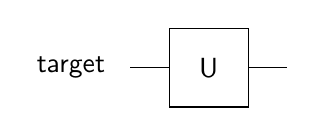
\begin{tikzpicture}[scale=.5] \node[draw=none] at (-3.5, 0) {target}; \draw (-2,0) -- (-1, 0); \draw (1, 0) -- (2, 0); \draw (-1,-1)--(-1,1)--(1,1)--(1,-1)--cycle; \node[draw=none] at (0, 0) {U}; \end{tikzpicture} } \]


\begin{DoxyParams}[1]{Parameters}
\mbox{\tt in,out}  & {\em multi\+Qubit} & object representing the set of all qubits \\
\hline
\mbox{\tt in}  & {\em target\+Qubit} & qubit to operate on \\
\hline
\mbox{\tt in}  & {\em alpha} & complex unitary parameter (row 1, column 1) \\
\hline
\mbox{\tt in}  & {\em beta} & complex unitary parameter (row 2, column 1) \\
\hline
\end{DoxyParams}

\begin{DoxyExceptions}{Exceptions}
{\em exit\+With\+Error} & if {\ttfamily target\+Qubit} is outside \mbox{[}0, {\ttfamily multi\+Qubit.\+num\+Qubits}), or if {\ttfamily alpha}, {\ttfamily beta} don\textquotesingle{}t satisfy $\vert${\ttfamily alpha$\vert$$^\wedge$2} + $\vert${\ttfamily beta$\vert$$^\wedge$2} = 1. \\
\hline
\end{DoxyExceptions}


Definition at line 98 of file Qu\+E\+S\+T\+\_\+env\+\_\+local.\+c.



References Multi\+Qubit\+::chunk\+Id, chunk\+Is\+Upper(), compact\+Unitary\+Distributed(), compact\+Unitary\+Local(), exchange\+State\+Vectors(), get\+Chunk\+Pair\+Id(), get\+Rot\+Angle(), half\+Matrix\+Block\+Fits\+In\+Chunk(), Multi\+Qubit\+::num\+Amps\+Per\+Chunk, Multi\+Qubit\+::num\+Qubits, Multi\+Qubit\+::pair\+State\+Vec, Qu\+E\+S\+T\+Assert(), R\+E\+AL, Multi\+Qubit\+::state\+Vec, and validate\+Alpha\+Beta().



Referenced by main(), rotate\+Around\+Axis(), test\+\_\+compact\+Unitary(), and test\+\_\+unitary().


\begin{DoxyCode}
99 \{
100     \mbox{\hyperlink{QuEST__env__local_8c_a3587b9d533e633ccf1abf9ad2ce45d8d}{QuESTAssert}}(targetQubit >= 0 && targetQubit < multiQubit.
      \mbox{\hyperlink{structMultiQubit_ab5b9795bdc6fb5855e1974dcbbaeb36f}{numQubits}}, 1, \_\_func\_\_);
101     \mbox{\hyperlink{QuEST__env__local_8c_a3587b9d533e633ccf1abf9ad2ce45d8d}{QuESTAssert}}(\mbox{\hyperlink{QuEST_8c_ae2b2c14a07dd7d50ff86032a3ca101d7}{validateAlphaBeta}}(alpha, beta), 6, \_\_func\_\_);
102 
103     \textcolor{comment}{// all values required to update state vector lie in this rank}
104     \mbox{\hyperlink{QuEST_8c_a9cee2d8716667a3318420a3b672f5b92}{compactUnitaryLocal}}(multiQubit, targetQubit, alpha, beta);
105 \}
\end{DoxyCode}
\mbox{\Hypertarget{QuEST_8h_ab4812953bc457405b3aa05a4c2f64f4a}\label{QuEST_8h_ab4812953bc457405b3aa05a4c2f64f4a}} 
\index{Qu\+E\+S\+T.\+h@{Qu\+E\+S\+T.\+h}!controlled\+Compact\+Unitary@{controlled\+Compact\+Unitary}}
\index{controlled\+Compact\+Unitary@{controlled\+Compact\+Unitary}!Qu\+E\+S\+T.\+h@{Qu\+E\+S\+T.\+h}}
\paragraph{\texorpdfstring{controlled\+Compact\+Unitary()}{controlledCompactUnitary()}}
{\footnotesize\ttfamily void controlled\+Compact\+Unitary (\begin{DoxyParamCaption}\item[{\mbox{\hyperlink{structMultiQubit}{Multi\+Qubit}}}]{multi\+Qubit,  }\item[{const int}]{control\+Qubit,  }\item[{const int}]{target\+Qubit,  }\item[{\mbox{\hyperlink{structComplex}{Complex}}}]{alpha,  }\item[{\mbox{\hyperlink{structComplex}{Complex}}}]{beta }\end{DoxyParamCaption})}



Apply a controlled unitary (single control, single target) parameterised by two given complex scalars. 

Given valid complex numbers $\alpha$ and $\beta$, applies the two-\/qubit unitary \[ \begin{pmatrix} 1 \\ & 1 \\ & & \alpha & -\beta^* \\ & & \beta & \alpha^* \end{pmatrix} \] to the control and target qubits. Valid $\alpha$, $\beta$ satisfy $|\alpha|^2 + |\beta|^2 = 1$. The target unitary is general up to a global phase factor. ~\newline
 \[ \setlength{\fboxrule}{0.01pt} \fbox{ 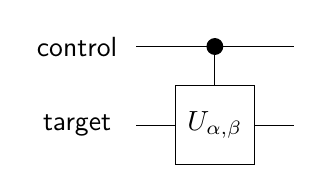
\begin{tikzpicture}[scale=.5] \node[draw=none] at (-3.5, 2) {control}; \node[draw=none] at (-3.5, 0) {target}; \draw (-2, 2) -- (2, 2); \draw[fill=black] (0, 2) circle (.2); \draw (0, 2) -- (0, 1); \draw (-2,0) -- (-1, 0); \draw (1, 0) -- (2, 0); \draw (-1,-1)--(-1,1)--(1,1)--(1,-1)--cycle; \node[draw=none] at (0, 0) {$U_{\alpha, \beta}$}; \end{tikzpicture} } \]


\begin{DoxyParams}[1]{Parameters}
\mbox{\tt in,out}  & {\em multi\+Qubit} & object representing the set of all qubits \\
\hline
\mbox{\tt in}  & {\em control\+Qubit} & apply the target unitary if this qubit has value 1 \\
\hline
\mbox{\tt in}  & {\em target\+Qubit} & qubit on which to apply the target unitary \\
\hline
\mbox{\tt in}  & {\em alpha} & complex unitary parameter (row 1, column 1) \\
\hline
\mbox{\tt in}  & {\em beta} & complex unitary parameter (row 2, column 1) \\
\hline
\end{DoxyParams}

\begin{DoxyExceptions}{Exceptions}
{\em exit\+With\+Error} & if either {\ttfamily control\+Qubit} or {\ttfamily target\+Qubit} are outside \mbox{[}0, {\ttfamily multi\+Qubit.\+num\+Qubits}) or are equal, or if {\ttfamily alpha}, {\ttfamily beta} don\textquotesingle{}t satisfy $\vert${\ttfamily alpha$\vert$$^\wedge$2} + $\vert${\ttfamily beta$\vert$$^\wedge$2} = 1. \\
\hline
\end{DoxyExceptions}


Definition at line 116 of file Qu\+E\+S\+T\+\_\+env\+\_\+local.\+c.



References Multi\+Qubit\+::chunk\+Id, chunk\+Is\+Upper(), controlled\+Compact\+Unitary\+Distributed(), controlled\+Compact\+Unitary\+Local(), exchange\+State\+Vectors(), get\+Chunk\+Pair\+Id(), get\+Rot\+Angle(), half\+Matrix\+Block\+Fits\+In\+Chunk(), Multi\+Qubit\+::num\+Amps\+Per\+Chunk, Multi\+Qubit\+::num\+Qubits, Multi\+Qubit\+::pair\+State\+Vec, Qu\+E\+S\+T\+Assert(), R\+E\+AL, Multi\+Qubit\+::state\+Vec, and validate\+Alpha\+Beta().



Referenced by controlled\+Rotate\+Around\+Axis(), main(), test\+\_\+controlled\+Compact\+Unitary(), test\+\_\+controlled\+Unitary(), and test\+\_\+multi\+Controlled\+Unitary().


\begin{DoxyCode}
117 \{
118     \mbox{\hyperlink{QuEST__env__local_8c_a3587b9d533e633ccf1abf9ad2ce45d8d}{QuESTAssert}}(targetQubit >= 0 && targetQubit < multiQubit.
      \mbox{\hyperlink{structMultiQubit_ab5b9795bdc6fb5855e1974dcbbaeb36f}{numQubits}}, 1, \_\_func\_\_);
119     \mbox{\hyperlink{QuEST__env__local_8c_a3587b9d533e633ccf1abf9ad2ce45d8d}{QuESTAssert}}(controlQubit >= 0 && controlQubit < multiQubit.
      \mbox{\hyperlink{structMultiQubit_ab5b9795bdc6fb5855e1974dcbbaeb36f}{numQubits}}, 2, \_\_func\_\_);
120     \mbox{\hyperlink{QuEST__env__local_8c_a3587b9d533e633ccf1abf9ad2ce45d8d}{QuESTAssert}}(controlQubit != targetQubit, 3, \_\_func\_\_);
121     \mbox{\hyperlink{QuEST__env__local_8c_a3587b9d533e633ccf1abf9ad2ce45d8d}{QuESTAssert}}(\mbox{\hyperlink{QuEST_8c_ae2b2c14a07dd7d50ff86032a3ca101d7}{validateAlphaBeta}}(alpha, beta), 6, \_\_func\_\_);
122 
123 
124     \mbox{\hyperlink{QuEST_8c_afc77657651d52c47403b44b923a098a8}{controlledCompactUnitaryLocal}}(multiQubit, controlQubit, targetQubit, alpha
      , beta);
125 \}
\end{DoxyCode}
\mbox{\Hypertarget{QuEST_8h_a67576895bbc65463481a8ea24d9b1e22}\label{QuEST_8h_a67576895bbc65463481a8ea24d9b1e22}} 
\index{Qu\+E\+S\+T.\+h@{Qu\+E\+S\+T.\+h}!controlled\+Not@{controlled\+Not}}
\index{controlled\+Not@{controlled\+Not}!Qu\+E\+S\+T.\+h@{Qu\+E\+S\+T.\+h}}
\paragraph{\texorpdfstring{controlled\+Not()}{controlledNot()}}
{\footnotesize\ttfamily void controlled\+Not (\begin{DoxyParamCaption}\item[{\mbox{\hyperlink{structMultiQubit}{Multi\+Qubit}}}]{multi\+Qubit,  }\item[{const int}]{control\+Qubit,  }\item[{const int}]{target\+Qubit }\end{DoxyParamCaption})}



Apply the controlled not (single control, single target) gate, also known as the c-\/X, c-\/sigma-\/X, c-\/\+Pauli-\/X and c-\/bit-\/flip gate. 

This applies sigmaX to the target qubit if the control qubit has value 1. This effects the two-\/qubit unitary \[ \begin{pmatrix} 1 \\ & 1 \\\ & & & 1 \\ & & 1 \end{pmatrix} \] on the control and target qubits.

\[ \setlength{\fboxrule}{0.01pt} \fbox{ 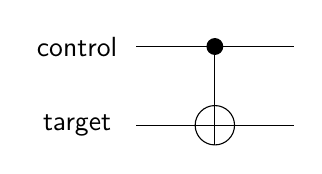
\begin{tikzpicture}[scale=.5] \node[draw=none] at (-3.5, 2) {control}; \node[draw=none] at (-3.5, 0) {target}; \draw (-2, 2) -- (2, 2); \draw[fill=black] (0, 2) circle (.2); \draw (0, 2) -- (0, -.5); \draw (-2,0) -- (2, 0); \draw (0, 0) circle (.5); \end{tikzpicture} } \] ~\newline
 
\begin{DoxyParams}[1]{Parameters}
\mbox{\tt in,out}  & {\em multi\+Qubit} & object representing the set of all qubits \\
\hline
\mbox{\tt in}  & {\em control\+Qubit} & nots the target if this qubit is 1 \\
\hline
\mbox{\tt in}  & {\em target\+Qubit} & qubit to not \\
\hline
\end{DoxyParams}

\begin{DoxyExceptions}{Exceptions}
{\em exit\+With\+Error} & if either {\ttfamily control\+Qubit} or {\ttfamily target\+Qubit} are outside \mbox{[}0, {\ttfamily multi\+Qubit.\+num\+Qubits}), or are equal. \\
\hline
\end{DoxyExceptions}


Definition at line 175 of file Qu\+E\+S\+T\+\_\+env\+\_\+local.\+c.



References Multi\+Qubit\+::chunk\+Id, chunk\+Is\+Upper(), controlled\+Not\+Distributed(), controlled\+Not\+Local(), exchange\+State\+Vectors(), get\+Chunk\+Pair\+Id(), half\+Matrix\+Block\+Fits\+In\+Chunk(), Multi\+Qubit\+::num\+Amps\+Per\+Chunk, Multi\+Qubit\+::num\+Qubits, Multi\+Qubit\+::pair\+State\+Vec, Qu\+E\+S\+T\+Assert(), R\+E\+AL, and Multi\+Qubit\+::state\+Vec.



Referenced by main(), and test\+\_\+controlled\+Not().


\begin{DoxyCode}
176 \{
177     \mbox{\hyperlink{QuEST__env__local_8c_a3587b9d533e633ccf1abf9ad2ce45d8d}{QuESTAssert}}(targetQubit >= 0 && targetQubit < multiQubit.
      \mbox{\hyperlink{structMultiQubit_ab5b9795bdc6fb5855e1974dcbbaeb36f}{numQubits}}, 1, \_\_func\_\_);
178     \mbox{\hyperlink{QuEST__env__local_8c_a3587b9d533e633ccf1abf9ad2ce45d8d}{QuESTAssert}}(controlQubit >= 0 && controlQubit < multiQubit.
      \mbox{\hyperlink{structMultiQubit_ab5b9795bdc6fb5855e1974dcbbaeb36f}{numQubits}}, 2, \_\_func\_\_);
179     \mbox{\hyperlink{QuEST__env__local_8c_a3587b9d533e633ccf1abf9ad2ce45d8d}{QuESTAssert}}(controlQubit != targetQubit, 3, \_\_func\_\_);
180     \mbox{\hyperlink{QuEST_8c_ad357a43e80e3baf013975b1b70942f4c}{controlledNotLocal}}(multiQubit, controlQubit, targetQubit);
181 \}
\end{DoxyCode}
\mbox{\Hypertarget{QuEST_8h_a11a96159191cbf1b01a1080e7f045aac}\label{QuEST_8h_a11a96159191cbf1b01a1080e7f045aac}} 
\index{Qu\+E\+S\+T.\+h@{Qu\+E\+S\+T.\+h}!controlled\+Phase\+Gate@{controlled\+Phase\+Gate}}
\index{controlled\+Phase\+Gate@{controlled\+Phase\+Gate}!Qu\+E\+S\+T.\+h@{Qu\+E\+S\+T.\+h}}
\paragraph{\texorpdfstring{controlled\+Phase\+Gate()}{controlledPhaseGate()}}
{\footnotesize\ttfamily void controlled\+Phase\+Gate (\begin{DoxyParamCaption}\item[{\mbox{\hyperlink{structMultiQubit}{Multi\+Qubit}}}]{multi\+Qubit,  }\item[{const int}]{id\+Qubit1,  }\item[{const int}]{id\+Qubit2 }\end{DoxyParamCaption})}



Apply the (two-\/qubit) controlled phase gate, also known as the controlled sigmaZ gate. 

For each state, if both input qubits have value one, multiply the amplitude of that state by -\/1. This applies the two-\/qubit unitary\+: \[ \begin{pmatrix} 1 \\ & 1 \\\ & & 1 \\ & & & -1 \end{pmatrix} \]

\[ \setlength{\fboxrule}{0.01pt} \fbox{ 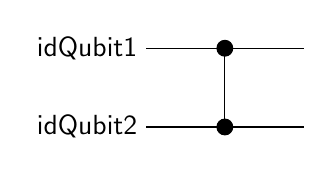
\begin{tikzpicture}[scale=.5] \node[draw=none] at (-3.5, 2) {idQubit1}; \node[draw=none] at (-3.5, 0) {idQubit2}; \draw (-2, 2) -- (2, 2); \draw[fill=black] (0, 2) circle (.2); \draw (0, 2) -- (0, 0); \draw (-2,0) -- (2, 0); \draw[fill=black] (0, 0) circle (.2); \end{tikzpicture} } \]


\begin{DoxyParams}[1]{Parameters}
\mbox{\tt in,out}  & {\em multi\+Qubit} & object representing the set of all qubits \\
\hline
\mbox{\tt in}  & {\em id\+Qubit1,id\+Qubit2} & qubits to operate upon \\
\hline
\end{DoxyParams}

\begin{DoxyExceptions}{Exceptions}
{\em exit\+With\+Error} & if {\ttfamily id\+Qubit1} or {\ttfamily id\+Qubit2} are outside \mbox{[}0, {\ttfamily multi\+Qubit.\+num\+Qubits}), or are equal \\
\hline
\end{DoxyExceptions}


Definition at line 1748 of file Qu\+E\+S\+T.\+c.



References Multi\+Qubit\+::chunk\+Id, extract\+Bit(), Complex\+Array\+::imag, Multi\+Qubit\+::num\+Amps\+Per\+Chunk, Multi\+Qubit\+::num\+Qubits, Qu\+E\+S\+T\+Assert(), Complex\+Array\+::real, R\+E\+AL, and Multi\+Qubit\+::state\+Vec.



Referenced by test\+\_\+controlled\+Phase\+Gate().


\begin{DoxyCode}
1749 \{
1750     \textcolor{keywordtype}{long} \textcolor{keywordtype}{long} \textcolor{keywordtype}{int} index;
1751     \textcolor{keywordtype}{long} \textcolor{keywordtype}{long} \textcolor{keywordtype}{int} stateVecSize;
1752     \textcolor{keywordtype}{int} bit1, bit2;
1753 
1754     \textcolor{keyword}{const} \textcolor{keywordtype}{long} \textcolor{keywordtype}{long} \textcolor{keywordtype}{int} chunkSize=multiQubit.\mbox{\hyperlink{structMultiQubit_a1cad83601a78635dd278259c7ed54f18}{numAmpsPerChunk}};
1755     \textcolor{keyword}{const} \textcolor{keywordtype}{long} \textcolor{keywordtype}{long} \textcolor{keywordtype}{int} chunkId=multiQubit.\mbox{\hyperlink{structMultiQubit_ab10c88249fa3825d6227ceec01d37e37}{chunkId}};
1756 
1757     \mbox{\hyperlink{QuEST__env__local_8c_a3587b9d533e633ccf1abf9ad2ce45d8d}{QuESTAssert}}(idQubit1 >= 0 && idQubit1 < multiQubit.\mbox{\hyperlink{structMultiQubit_ab5b9795bdc6fb5855e1974dcbbaeb36f}{numQubits}}, 2, \_\_func\_\_);
1758     \mbox{\hyperlink{QuEST__env__local_8c_a3587b9d533e633ccf1abf9ad2ce45d8d}{QuESTAssert}}(idQubit2 >= 0 && idQubit2 < multiQubit.\mbox{\hyperlink{structMultiQubit_ab5b9795bdc6fb5855e1974dcbbaeb36f}{numQubits}}, 1, \_\_func\_\_);
1759     \mbox{\hyperlink{QuEST__env__local_8c_a3587b9d533e633ccf1abf9ad2ce45d8d}{QuESTAssert}}(idQubit1 != idQubit2, 3, \_\_func\_\_);
1760 
1761     \textcolor{comment}{// dimension of the state vector}
1762     stateVecSize = multiQubit.\mbox{\hyperlink{structMultiQubit_a1cad83601a78635dd278259c7ed54f18}{numAmpsPerChunk}};
1763     \mbox{\hyperlink{QuEST__precision_8h_a4b654506f18b8bfd61ad2a29a7e38c25}{REAL}} *stateVecReal = multiQubit.\mbox{\hyperlink{structMultiQubit_a45483190d6b01ef6b2f98f2bec9ab94f}{stateVec}}.\mbox{\hyperlink{structComplexArray_a4195cac6c784ea1b6271f1c7dba1548a}{real}};
1764     \mbox{\hyperlink{QuEST__precision_8h_a4b654506f18b8bfd61ad2a29a7e38c25}{REAL}} *stateVecImag = multiQubit.\mbox{\hyperlink{structMultiQubit_a45483190d6b01ef6b2f98f2bec9ab94f}{stateVec}}.\mbox{\hyperlink{structComplexArray_a79dde47c7ae530c79cebfdf57b225968}{imag}};
1765 
1766 \textcolor{preprocessor}{# ifdef \_OPENMP}
1767 \textcolor{preprocessor}{# pragma omp parallel for \(\backslash\)}
1768 \textcolor{preprocessor}{    default  (none)                          \(\backslash\)}
1769 \textcolor{preprocessor}{    shared   (stateVecSize, stateVecReal,stateVecImag ) \(\backslash\)}
1770 \textcolor{preprocessor}{    private  (index,bit1,bit2)                 \(\backslash\)}
1771 \textcolor{preprocessor}{    schedule (static)}
1772 \textcolor{preprocessor}{# endif}
1773     \textcolor{keywordflow}{for} (index=0; index<stateVecSize; index++) \{
1774         bit1 = \mbox{\hyperlink{QuEST_8c_a100463f6ec212c76a5fad99579000505}{extractBit}} (idQubit1, index+chunkId*chunkSize);
1775         bit2 = \mbox{\hyperlink{QuEST_8c_a100463f6ec212c76a5fad99579000505}{extractBit}} (idQubit2, index+chunkId*chunkSize);
1776         \textcolor{keywordflow}{if} (bit1 && bit2) \{
1777             stateVecReal [index] = - stateVecReal [index];
1778             stateVecImag [index] = - stateVecImag [index];
1779         \}
1780     \}
1781 \}
\end{DoxyCode}
\mbox{\Hypertarget{QuEST_8h_ad41f82b41149393a642391b67b3a287e}\label{QuEST_8h_ad41f82b41149393a642391b67b3a287e}} 
\index{Qu\+E\+S\+T.\+h@{Qu\+E\+S\+T.\+h}!controlled\+Rotate\+Around\+Axis@{controlled\+Rotate\+Around\+Axis}}
\index{controlled\+Rotate\+Around\+Axis@{controlled\+Rotate\+Around\+Axis}!Qu\+E\+S\+T.\+h@{Qu\+E\+S\+T.\+h}}
\paragraph{\texorpdfstring{controlled\+Rotate\+Around\+Axis()}{controlledRotateAroundAxis()}}
{\footnotesize\ttfamily void controlled\+Rotate\+Around\+Axis (\begin{DoxyParamCaption}\item[{\mbox{\hyperlink{structMultiQubit}{Multi\+Qubit}}}]{multi\+Qubit,  }\item[{const int}]{control\+Qubit,  }\item[{const int}]{target\+Qubit,  }\item[{\mbox{\hyperlink{QuEST__precision_8h_a4b654506f18b8bfd61ad2a29a7e38c25}{R\+E\+AL}}}]{angle,  }\item[{\mbox{\hyperlink{structVector}{Vector}}}]{axis }\end{DoxyParamCaption})}



Applies a controlled rotation by a given angle around a given vector on the Bloch-\/sphere. 

The vector must not be zero (else an error is thrown), but needn\textquotesingle{}t be unit magnitude.

For angle $\theta$ and axis vector $\vec{n}$, applies $R_{\hat{n}} = \exp \left(- i \frac{\theta}{2} \hat{n} \cdot \vec{\sigma} \right) $ to states where the target qubit is 1 ( $\vec{\sigma}$ is the vector of Pauli matrices).

\[ \setlength{\fboxrule}{0.01pt} \fbox{ 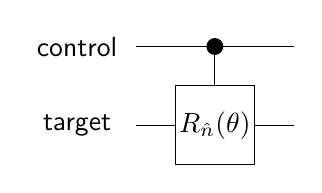
\begin{tikzpicture}[scale=.5] \node[draw=none] at (-3.5, 2) {control}; \node[draw=none] at (-3.5, 0) {target}; \draw (-2, 2) -- (2, 2); \draw[fill=black] (0, 2) circle (.2); \draw (0, 2) -- (0, 1); \draw (-2,0) -- (-1, 0); \draw (1, 0) -- (2, 0); \draw (-1,-1)--(-1,1)--(1,1)--(1,-1)--cycle; \node[draw=none] at (0, 0) {$R_{\hat{n}}(\theta)$}; \end{tikzpicture} } \]


\begin{DoxyParams}[1]{Parameters}
\mbox{\tt in,out}  & {\em multi\+Qubit} & object representing the set of all qubits \\
\hline
\mbox{\tt in}  & {\em control\+Qubit} & qubit with value 1 in the rotated states \\
\hline
\mbox{\tt in}  & {\em target\+Qubit} & qubit to rotate \\
\hline
\mbox{\tt in}  & {\em angle} & angle by which to rotate in radians \\
\hline
\mbox{\tt in}  & {\em axis} & vector around which to rotate (can be non-\/unit; will be normalised) \\
\hline
\end{DoxyParams}

\begin{DoxyExceptions}{Exceptions}
{\em exit\+With\+Error} & if either {\ttfamily control\+Qubit} or {\ttfamily target\+Qubit} are outside \mbox{[}0, {\ttfamily multi\+Qubit.\+num\+Qubits}) or are equal or if {\ttfamily axis} is the zero vector \\
\hline
\end{DoxyExceptions}


Definition at line 459 of file Qu\+E\+S\+T.\+c.



References controlled\+Compact\+Unitary(), Complex\+::imag, Complex\+::real, Vector\+::x, Vector\+::y, and Vector\+::z.



Referenced by controlled\+Rotate\+X(), controlled\+Rotate\+Y(), and controlled\+Rotate\+Z().


\begin{DoxyCode}
459                                                                                                            
                         \{
460 
461     \textcolor{keywordtype}{double} mag = sqrt(pow(axis.\mbox{\hyperlink{structVector_aac7abe171ba4bada50ed72acba6259fc}{x}},2) + pow(axis.\mbox{\hyperlink{structVector_a375ca805d4c808a53d7c4e0c737ae3de}{y}},2) + pow(axis.\mbox{\hyperlink{structVector_ad4e863651be7d6b7e2b28cd7445a0ccf}{z}},2));
462     \mbox{\hyperlink{structVector}{Vector}} unitAxis = \{axis.\mbox{\hyperlink{structVector_aac7abe171ba4bada50ed72acba6259fc}{x}}/mag, axis.\mbox{\hyperlink{structVector_a375ca805d4c808a53d7c4e0c737ae3de}{y}}/mag, axis.\mbox{\hyperlink{structVector_ad4e863651be7d6b7e2b28cd7445a0ccf}{z}}/mag\};
463 
464     \mbox{\hyperlink{structComplex}{Complex}} alpha, beta;
465     alpha.\mbox{\hyperlink{structComplex_a479ad939835457595fcca3ca55c06283}{real}} = cos(angle/2.0);
466     alpha.\mbox{\hyperlink{structComplex_a1151948284b21c0052f203f23ab931d9}{imag}} = -sin(angle/2.0)*unitAxis.\mbox{\hyperlink{structVector_ad4e863651be7d6b7e2b28cd7445a0ccf}{z}};       
467     beta.\mbox{\hyperlink{structComplex_a479ad939835457595fcca3ca55c06283}{real}} = sin(angle/2.0)*unitAxis.\mbox{\hyperlink{structVector_a375ca805d4c808a53d7c4e0c737ae3de}{y}};
468     beta.\mbox{\hyperlink{structComplex_a1151948284b21c0052f203f23ab931d9}{imag}} = -sin(angle/2.0)*unitAxis.\mbox{\hyperlink{structVector_aac7abe171ba4bada50ed72acba6259fc}{x}};
469     \mbox{\hyperlink{QuEST__env__local_8c_ab4812953bc457405b3aa05a4c2f64f4a}{controlledCompactUnitary}}(multiQubit, controlQubit, targetQubit, alpha, beta);
470 \}
\end{DoxyCode}
\mbox{\Hypertarget{QuEST_8h_ac6923ac57e67d9a21096e06f6a9012f6}\label{QuEST_8h_ac6923ac57e67d9a21096e06f6a9012f6}} 
\index{Qu\+E\+S\+T.\+h@{Qu\+E\+S\+T.\+h}!controlled\+RotateX@{controlled\+RotateX}}
\index{controlled\+RotateX@{controlled\+RotateX}!Qu\+E\+S\+T.\+h@{Qu\+E\+S\+T.\+h}}
\paragraph{\texorpdfstring{controlled\+Rotate\+X()}{controlledRotateX()}}
{\footnotesize\ttfamily void controlled\+RotateX (\begin{DoxyParamCaption}\item[{\mbox{\hyperlink{structMultiQubit}{Multi\+Qubit}}}]{multi\+Qubit,  }\item[{const int}]{control\+Qubit,  }\item[{const int}]{target\+Qubit,  }\item[{\mbox{\hyperlink{QuEST__precision_8h_a4b654506f18b8bfd61ad2a29a7e38c25}{R\+E\+AL}}}]{angle }\end{DoxyParamCaption})}



Applies a controlled rotation by a given angle around the X-\/axis of the Bloch-\/sphere. 

The target qubit is rotated in states where the control qubit has value 1.

\[ \setlength{\fboxrule}{0.01pt} \fbox{ 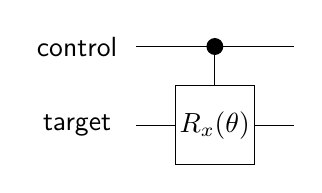
\begin{tikzpicture}[scale=.5] \node[draw=none] at (-3.5, 2) {control}; \node[draw=none] at (-3.5, 0) {target}; \draw (-2, 2) -- (2, 2); \draw[fill=black] (0, 2) circle (.2); \draw (0, 2) -- (0, 1); \draw (-2,0) -- (-1, 0); \draw (1, 0) -- (2, 0); \draw (-1,-1)--(-1,1)--(1,1)--(1,-1)--cycle; \node[draw=none] at (0, 0) {$R_x(\theta)$}; \end{tikzpicture} } \] ~\newline
 
\begin{DoxyParams}[1]{Parameters}
\mbox{\tt in,out}  & {\em multi\+Qubit} & object representing the set of all qubits \\
\hline
\mbox{\tt in}  & {\em control\+Qubit} & qubit which has value 1 in the rotated states \\
\hline
\mbox{\tt in}  & {\em tagret\+Qubit} & qubit to rotate \\
\hline
\mbox{\tt in}  & {\em angle} & angle by which to rotate the target qubit in radians \\
\hline
\end{DoxyParams}

\begin{DoxyExceptions}{Exceptions}
{\em exit\+With\+Error} & if either {\ttfamily control\+Qubit} or {\ttfamily target\+Qubit} are outside \mbox{[}0, {\ttfamily multi\+Qubit.\+num\+Qubits}) or are equal. \\
\hline
\end{DoxyExceptions}


Definition at line 472 of file Qu\+E\+S\+T.\+c.



References controlled\+Rotate\+Around\+Axis().


\begin{DoxyCode}
472                                                                                                         \{
473 
474     \mbox{\hyperlink{structVector}{Vector}} unitAxis = \{1, 0, 0\};
475     \mbox{\hyperlink{QuEST_8c_ad41f82b41149393a642391b67b3a287e}{controlledRotateAroundAxis}}(multiQubit, controlQubit, targetQubit, angle, 
      unitAxis);
476 \}
\end{DoxyCode}
\mbox{\Hypertarget{QuEST_8h_a71e90a2f7292116338c062934f9d1202}\label{QuEST_8h_a71e90a2f7292116338c062934f9d1202}} 
\index{Qu\+E\+S\+T.\+h@{Qu\+E\+S\+T.\+h}!controlled\+RotateY@{controlled\+RotateY}}
\index{controlled\+RotateY@{controlled\+RotateY}!Qu\+E\+S\+T.\+h@{Qu\+E\+S\+T.\+h}}
\paragraph{\texorpdfstring{controlled\+Rotate\+Y()}{controlledRotateY()}}
{\footnotesize\ttfamily void controlled\+RotateY (\begin{DoxyParamCaption}\item[{\mbox{\hyperlink{structMultiQubit}{Multi\+Qubit}}}]{multi\+Qubit,  }\item[{const int}]{control\+Qubit,  }\item[{const int}]{target\+Qubit,  }\item[{\mbox{\hyperlink{QuEST__precision_8h_a4b654506f18b8bfd61ad2a29a7e38c25}{R\+E\+AL}}}]{angle }\end{DoxyParamCaption})}



Applies a controlled rotation by a given angle around the Y-\/axis of the Bloch-\/sphere. 

The target qubit is rotated in states where the control qubit has value 1.

\[ \setlength{\fboxrule}{0.01pt} \fbox{ 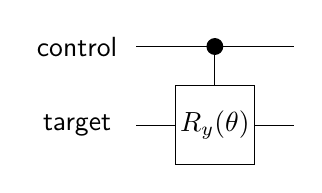
\begin{tikzpicture}[scale=.5] \node[draw=none] at (-3.5, 2) {control}; \node[draw=none] at (-3.5, 0) {target}; \draw (-2, 2) -- (2, 2); \draw[fill=black] (0, 2) circle (.2); \draw (0, 2) -- (0, 1); \draw (-2,0) -- (-1, 0); \draw (1, 0) -- (2, 0); \draw (-1,-1)--(-1,1)--(1,1)--(1,-1)--cycle; \node[draw=none] at (0, 0) {$R_y(\theta)$}; \end{tikzpicture} } \] ~\newline
 
\begin{DoxyParams}[1]{Parameters}
\mbox{\tt in,out}  & {\em multi\+Qubit} & object representing the set of all qubits \\
\hline
\mbox{\tt in}  & {\em control\+Qubit} & qubit which has value 1 in the rotated states \\
\hline
\mbox{\tt in}  & {\em tagret\+Qubit} & qubit to rotate \\
\hline
\mbox{\tt in}  & {\em angle} & angle by which to rotate the target qubit in radians \\
\hline
\end{DoxyParams}

\begin{DoxyExceptions}{Exceptions}
{\em exit\+With\+Error} & if either {\ttfamily control\+Qubit} or {\ttfamily target\+Qubit} are outside \mbox{[}0, {\ttfamily multi\+Qubit.\+num\+Qubits}) or are equal. \\
\hline
\end{DoxyExceptions}


Definition at line 478 of file Qu\+E\+S\+T.\+c.



References controlled\+Rotate\+Around\+Axis().


\begin{DoxyCode}
478                                                                                                         \{
479 
480     \mbox{\hyperlink{structVector}{Vector}} unitAxis = \{0, 1, 0\};
481     \mbox{\hyperlink{QuEST_8c_ad41f82b41149393a642391b67b3a287e}{controlledRotateAroundAxis}}(multiQubit, controlQubit, targetQubit, angle, 
      unitAxis);
482 \}
\end{DoxyCode}
\mbox{\Hypertarget{QuEST_8h_a668e5d2634b02e98bc73675ccb11d61c}\label{QuEST_8h_a668e5d2634b02e98bc73675ccb11d61c}} 
\index{Qu\+E\+S\+T.\+h@{Qu\+E\+S\+T.\+h}!controlled\+RotateZ@{controlled\+RotateZ}}
\index{controlled\+RotateZ@{controlled\+RotateZ}!Qu\+E\+S\+T.\+h@{Qu\+E\+S\+T.\+h}}
\paragraph{\texorpdfstring{controlled\+Rotate\+Z()}{controlledRotateZ()}}
{\footnotesize\ttfamily void controlled\+RotateZ (\begin{DoxyParamCaption}\item[{\mbox{\hyperlink{structMultiQubit}{Multi\+Qubit}}}]{multi\+Qubit,  }\item[{const int}]{control\+Qubit,  }\item[{const int}]{target\+Qubit,  }\item[{\mbox{\hyperlink{QuEST__precision_8h_a4b654506f18b8bfd61ad2a29a7e38c25}{R\+E\+AL}}}]{angle }\end{DoxyParamCaption})}



Applies a controlled rotation by a given angle around the Z-\/axis of the Bloch-\/sphere. 

The target qubit is rotated in states where the control qubit has value 1.

\[ \setlength{\fboxrule}{0.01pt} \fbox{ 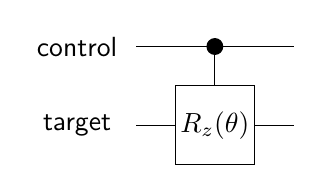
\begin{tikzpicture}[scale=.5] \node[draw=none] at (-3.5, 2) {control}; \node[draw=none] at (-3.5, 0) {target}; \draw (-2, 2) -- (2, 2); \draw[fill=black] (0, 2) circle (.2); \draw (0, 2) -- (0, 1); \draw (-2,0) -- (-1, 0); \draw (1, 0) -- (2, 0); \draw (-1,-1)--(-1,1)--(1,1)--(1,-1)--cycle; \node[draw=none] at (0, 0) {$R_z(\theta)$}; \end{tikzpicture} } \] ~\newline
 
\begin{DoxyParams}[1]{Parameters}
\mbox{\tt in,out}  & {\em multi\+Qubit} & object representing the set of all qubits \\
\hline
\mbox{\tt in}  & {\em control\+Qubit} & qubit which has value 1 in the rotated states \\
\hline
\mbox{\tt in}  & {\em tagret\+Qubit} & qubit to rotate \\
\hline
\mbox{\tt in}  & {\em angle} & angle by which to rotate the target qubit in radians \\
\hline
\end{DoxyParams}

\begin{DoxyExceptions}{Exceptions}
{\em exit\+With\+Error} & if either {\ttfamily control\+Qubit} or {\ttfamily target\+Qubit} are outside \mbox{[}0, {\ttfamily multi\+Qubit.\+num\+Qubits}) or are equal. \\
\hline
\end{DoxyExceptions}


Definition at line 484 of file Qu\+E\+S\+T.\+c.



References controlled\+Rotate\+Around\+Axis().


\begin{DoxyCode}
484                                                                                                         \{
485 
486     \mbox{\hyperlink{structVector}{Vector}} unitAxis = \{0, 0, 1\};
487     \mbox{\hyperlink{QuEST_8c_ad41f82b41149393a642391b67b3a287e}{controlledRotateAroundAxis}}(multiQubit, controlQubit, targetQubit, angle, 
      unitAxis);
488 \}
\end{DoxyCode}
\mbox{\Hypertarget{QuEST_8h_a8a701526263392599aa21d0d0f05d9d8}\label{QuEST_8h_a8a701526263392599aa21d0d0f05d9d8}} 
\index{Qu\+E\+S\+T.\+h@{Qu\+E\+S\+T.\+h}!controlled\+Unitary@{controlled\+Unitary}}
\index{controlled\+Unitary@{controlled\+Unitary}!Qu\+E\+S\+T.\+h@{Qu\+E\+S\+T.\+h}}
\paragraph{\texorpdfstring{controlled\+Unitary()}{controlledUnitary()}}
{\footnotesize\ttfamily void controlled\+Unitary (\begin{DoxyParamCaption}\item[{\mbox{\hyperlink{structMultiQubit}{Multi\+Qubit}}}]{multi\+Qubit,  }\item[{const int}]{control\+Qubit,  }\item[{const int}]{target\+Qubit,  }\item[{\mbox{\hyperlink{structComplexMatrix2}{Complex\+Matrix2}}}]{u }\end{DoxyParamCaption})}



Apply a general controlled unitary (single control, single target), which can include a global phase factor. 

The given unitary is applied to the target qubit if the control qubit has value 1, effecting the two-\/qubit unitary \[ \begin{pmatrix} 1 \\ & 1 \\ & & u_{00} & u_{01}\\ & & u_{10} & u_{11} \end{pmatrix} \] on the control and target qubits.

\[ \setlength{\fboxrule}{0.01pt} \fbox{ 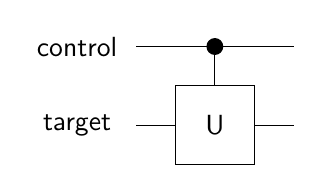
\begin{tikzpicture}[scale=.5] \node[draw=none] at (-3.5, 2) {control}; \node[draw=none] at (-3.5, 0) {target}; \draw (-2, 2) -- (2, 2); \draw[fill=black] (0, 2) circle (.2); \draw (0, 2) -- (0, 1); \draw (-2,0) -- (-1, 0); \draw (1, 0) -- (2, 0); \draw (-1,-1)--(-1,1)--(1,1)--(1,-1)--cycle; \node[draw=none] at (0, 0) {U}; \end{tikzpicture} } \]


\begin{DoxyParams}[1]{Parameters}
\mbox{\tt in,out}  & {\em multi\+Qubit} & object representing the set of all qubits \\
\hline
\mbox{\tt in}  & {\em control\+Qubit} & apply unitary if this qubit is 1 \\
\hline
\mbox{\tt in}  & {\em target\+Qubit} & qubit to operate on \\
\hline
\mbox{\tt in}  & {\em u} & single-\/qubit unitary matrix to apply \\
\hline
\end{DoxyParams}

\begin{DoxyExceptions}{Exceptions}
{\em exit\+With\+Error} & if either {\ttfamily control\+Qubit} or {\ttfamily target\+Qubit} are outside \mbox{[}0, {\ttfamily multi\+Qubit.\+num\+Qubits}) or are equal, or if {\ttfamily u} is not unitary. \\
\hline
\end{DoxyExceptions}


Definition at line 127 of file Qu\+E\+S\+T\+\_\+env\+\_\+local.\+c.



References Multi\+Qubit\+::chunk\+Id, chunk\+Is\+Upper(), controlled\+Unitary\+Distributed(), controlled\+Unitary\+Local(), exchange\+State\+Vectors(), get\+Chunk\+Pair\+Id(), get\+Rot\+Angle\+From\+Unitary\+Matrix(), half\+Matrix\+Block\+Fits\+In\+Chunk(), Multi\+Qubit\+::num\+Amps\+Per\+Chunk, Multi\+Qubit\+::num\+Qubits, Multi\+Qubit\+::pair\+State\+Vec, Qu\+E\+S\+T\+Assert(), R\+E\+AL, Multi\+Qubit\+::state\+Vec, and validate\+Matrix\+Is\+Unitary().



Referenced by test\+\_\+controlled\+Unitary().


\begin{DoxyCode}
128 \{
129     \mbox{\hyperlink{QuEST__env__local_8c_a3587b9d533e633ccf1abf9ad2ce45d8d}{QuESTAssert}}(targetQubit >= 0 && targetQubit < multiQubit.
      \mbox{\hyperlink{structMultiQubit_ab5b9795bdc6fb5855e1974dcbbaeb36f}{numQubits}}, 1, \_\_func\_\_);
130     \mbox{\hyperlink{QuEST__env__local_8c_a3587b9d533e633ccf1abf9ad2ce45d8d}{QuESTAssert}}(controlQubit >= 0 && controlQubit < multiQubit.
      \mbox{\hyperlink{structMultiQubit_ab5b9795bdc6fb5855e1974dcbbaeb36f}{numQubits}}, 2, \_\_func\_\_);
131     \mbox{\hyperlink{QuEST__env__local_8c_a3587b9d533e633ccf1abf9ad2ce45d8d}{QuESTAssert}}(controlQubit != targetQubit, 3, \_\_func\_\_);
132     \mbox{\hyperlink{QuEST__env__local_8c_a3587b9d533e633ccf1abf9ad2ce45d8d}{QuESTAssert}}(\mbox{\hyperlink{QuEST_8c_ae4fea133d1a8f09ff8da03038100adb2}{validateMatrixIsUnitary}}(u), 5, \_\_func\_\_);
133 
134     \mbox{\hyperlink{QuEST_8c_a8a4afcff70195a306c082b8ed8d4e09a}{controlledUnitaryLocal}}(multiQubit, controlQubit, targetQubit, u);
135 \}
\end{DoxyCode}
\mbox{\Hypertarget{QuEST_8h_a9c02591bc64c2918503afa231d90d83f}\label{QuEST_8h_a9c02591bc64c2918503afa231d90d83f}} 
\index{Qu\+E\+S\+T.\+h@{Qu\+E\+S\+T.\+h}!create\+Multi\+Qubit@{create\+Multi\+Qubit}}
\index{create\+Multi\+Qubit@{create\+Multi\+Qubit}!Qu\+E\+S\+T.\+h@{Qu\+E\+S\+T.\+h}}
\paragraph{\texorpdfstring{create\+Multi\+Qubit()}{createMultiQubit()}}
{\footnotesize\ttfamily void create\+Multi\+Qubit (\begin{DoxyParamCaption}\item[{\mbox{\hyperlink{structMultiQubit}{Multi\+Qubit}} $\ast$}]{multi\+Qubit,  }\item[{int}]{num\+Qubits,  }\item[{\mbox{\hyperlink{structQuESTEnv}{Qu\+E\+S\+T\+Env}}}]{env }\end{DoxyParamCaption})}



Create a \mbox{\hyperlink{structMultiQubit}{Multi\+Qubit}} object representing a set of qubits. 

Allocate space for state vector of probability amplitudes, including space for temporary values to be copied from one other chunk if running the distributed version. Define properties related to the size of the set of qubits. init\+State\+Zero should be called after this to initialise the qubits to the zero state.


\begin{DoxyParams}[1]{Parameters}
\mbox{\tt in,out}  & {\em multi\+Qubit} & a pointer to an object representing the set of qubits \\
\hline
\mbox{\tt in}  & {\em num\+Qubits} & number of qubits in the system \\
\hline
\mbox{\tt in}  & {\em env} & object representing the execution environment (local, multinode etc) \\
\hline
\end{DoxyParams}

\begin{DoxyExceptions}{Exceptions}
{\em exit\+With\+Error} & if {\ttfamily num\+Qubits} $<$= 0 \\
\hline
\end{DoxyExceptions}


Definition at line 44 of file Qu\+E\+S\+T.\+c.



References Multi\+Qubit\+::chunk\+Id, Multi\+Qubit\+::device\+State\+Vec, env, Multi\+Qubit\+::first\+Level\+Reduction, Complex\+Array\+::imag, Multi\+Qubit\+::num\+Amps\+Per\+Chunk, Multi\+Qubit\+::num\+Chunks, Multi\+Qubit\+::num\+Qubits, Qu\+E\+S\+T\+Env\+::num\+Ranks, Multi\+Qubit\+::pair\+State\+Vec, Qu\+E\+S\+T\+Assert(), Qu\+E\+S\+T\+Env\+::rank, Complex\+Array\+::real, R\+E\+AL, R\+E\+D\+U\+C\+E\+\_\+\+S\+H\+A\+R\+E\+D\+\_\+\+S\+I\+ZE, Multi\+Qubit\+::second\+Level\+Reduction, and Multi\+Qubit\+::state\+Vec.



Referenced by main(), test\+\_\+collapse\+To\+Outcome(), test\+\_\+compact\+Unitary(), test\+\_\+controlled\+Compact\+Unitary(), test\+\_\+controlled\+Not(), test\+\_\+controlled\+Phase\+Gate(), test\+\_\+controlled\+Unitary(), test\+\_\+find\+Probability\+Of\+Outcome(), test\+\_\+get\+Imag\+Amp\+El(), test\+\_\+get\+Prob\+El(), test\+\_\+get\+Real\+Amp\+El(), test\+\_\+hadamard(), test\+\_\+init\+Classical\+State(), test\+\_\+init\+State\+Plus(), test\+\_\+init\+State\+Zero(), test\+\_\+measure(), test\+\_\+measure\+With\+Stats(), test\+\_\+multi\+Controlled\+Phase\+Gate(), test\+\_\+multi\+Controlled\+Unitary(), test\+\_\+s\+Gate(), test\+\_\+sigma\+X(), test\+\_\+sigma\+Y(), test\+\_\+sigma\+Z(), test\+\_\+t\+Gate(), and test\+\_\+unitary().


\begin{DoxyCode}
45 \{
46     \mbox{\hyperlink{QuEST__env__local_8c_a3587b9d533e633ccf1abf9ad2ce45d8d}{QuESTAssert}}(numQubits>0, 9, \_\_func\_\_);
47     \textcolor{keywordtype}{long} \textcolor{keywordtype}{long} \textcolor{keywordtype}{int} numAmps = 1L << numQubits;
48     \textcolor{keywordtype}{long} \textcolor{keywordtype}{long} \textcolor{keywordtype}{int} numAmpsPerRank = numAmps/\mbox{\hyperlink{runTests_8c_a5fd8ba97fcae3408ae6221dfc3cc1f93}{env}}.\mbox{\hyperlink{structQuESTEnv_af22aacd7c9905accae28484785c193b4}{numRanks}};
49 
50     multiQubit->\mbox{\hyperlink{structMultiQubit_a45483190d6b01ef6b2f98f2bec9ab94f}{stateVec}}.\mbox{\hyperlink{structComplexArray_a4195cac6c784ea1b6271f1c7dba1548a}{real}} = malloc(numAmpsPerRank * \textcolor{keyword}{sizeof}(*(multiQubit->
      \mbox{\hyperlink{structMultiQubit_a45483190d6b01ef6b2f98f2bec9ab94f}{stateVec}}.\mbox{\hyperlink{structComplexArray_a4195cac6c784ea1b6271f1c7dba1548a}{real}})));
51     multiQubit->\mbox{\hyperlink{structMultiQubit_a45483190d6b01ef6b2f98f2bec9ab94f}{stateVec}}.\mbox{\hyperlink{structComplexArray_a79dde47c7ae530c79cebfdf57b225968}{imag}} = malloc(numAmpsPerRank * \textcolor{keyword}{sizeof}(*(multiQubit->
      \mbox{\hyperlink{structMultiQubit_a45483190d6b01ef6b2f98f2bec9ab94f}{stateVec}}.\mbox{\hyperlink{structComplexArray_a79dde47c7ae530c79cebfdf57b225968}{imag}})));
52     \textcolor{keywordflow}{if} (\mbox{\hyperlink{runTests_8c_a5fd8ba97fcae3408ae6221dfc3cc1f93}{env}}.\mbox{\hyperlink{structQuESTEnv_af22aacd7c9905accae28484785c193b4}{numRanks}}>1)\{
53         multiQubit->\mbox{\hyperlink{structMultiQubit_a76f7db4eab52d2b30f58f973ada809c5}{pairStateVec}}.\mbox{\hyperlink{structComplexArray_a4195cac6c784ea1b6271f1c7dba1548a}{real}} = malloc(numAmpsPerRank * \textcolor{keyword}{sizeof}(*(multiQubit->
      \mbox{\hyperlink{structMultiQubit_a76f7db4eab52d2b30f58f973ada809c5}{pairStateVec}}.\mbox{\hyperlink{structComplexArray_a4195cac6c784ea1b6271f1c7dba1548a}{real}})));
54         multiQubit->\mbox{\hyperlink{structMultiQubit_a76f7db4eab52d2b30f58f973ada809c5}{pairStateVec}}.\mbox{\hyperlink{structComplexArray_a79dde47c7ae530c79cebfdf57b225968}{imag}} = malloc(numAmpsPerRank * \textcolor{keyword}{sizeof}(*(multiQubit->
      \mbox{\hyperlink{structMultiQubit_a76f7db4eab52d2b30f58f973ada809c5}{pairStateVec}}.\mbox{\hyperlink{structComplexArray_a79dde47c7ae530c79cebfdf57b225968}{imag}})));
55     \}
56 
57     \textcolor{keywordflow}{if} ( (!(multiQubit->\mbox{\hyperlink{structMultiQubit_a45483190d6b01ef6b2f98f2bec9ab94f}{stateVec}}.\mbox{\hyperlink{structComplexArray_a4195cac6c784ea1b6271f1c7dba1548a}{real}}) || !(multiQubit->\mbox{\hyperlink{structMultiQubit_a45483190d6b01ef6b2f98f2bec9ab94f}{stateVec}}.
      \mbox{\hyperlink{structComplexArray_a79dde47c7ae530c79cebfdf57b225968}{imag}}))
58             && numAmpsPerRank ) \{
59         printf(\textcolor{stringliteral}{"Could not allocate memory!"});
60         exit (EXIT\_FAILURE);
61     \}
62 
63     \textcolor{keywordflow}{if} ( \mbox{\hyperlink{runTests_8c_a5fd8ba97fcae3408ae6221dfc3cc1f93}{env}}.\mbox{\hyperlink{structQuESTEnv_af22aacd7c9905accae28484785c193b4}{numRanks}}>1 && (!(multiQubit->\mbox{\hyperlink{structMultiQubit_a76f7db4eab52d2b30f58f973ada809c5}{pairStateVec}}.
      \mbox{\hyperlink{structComplexArray_a4195cac6c784ea1b6271f1c7dba1548a}{real}}) || !(multiQubit->\mbox{\hyperlink{structMultiQubit_a76f7db4eab52d2b30f58f973ada809c5}{pairStateVec}}.\mbox{\hyperlink{structComplexArray_a79dde47c7ae530c79cebfdf57b225968}{imag}}))
64             && numAmpsPerRank ) \{
65         printf(\textcolor{stringliteral}{"Could not allocate memory!"});
66         exit (EXIT\_FAILURE);
67     \}
68 
69     multiQubit->\mbox{\hyperlink{structMultiQubit_ab5b9795bdc6fb5855e1974dcbbaeb36f}{numQubits}} = numQubits;
70     multiQubit->\mbox{\hyperlink{structMultiQubit_a1cad83601a78635dd278259c7ed54f18}{numAmpsPerChunk}} = numAmpsPerRank;
71     multiQubit->\mbox{\hyperlink{structMultiQubit_ab10c88249fa3825d6227ceec01d37e37}{chunkId}} = \mbox{\hyperlink{runTests_8c_a5fd8ba97fcae3408ae6221dfc3cc1f93}{env}}.\mbox{\hyperlink{structQuESTEnv_aa648bb336cf8598467cb62db00b9cee8}{rank}};
72     multiQubit->\mbox{\hyperlink{structMultiQubit_acd43f2f57991709c9e94f73662c972b2}{numChunks}} = \mbox{\hyperlink{runTests_8c_a5fd8ba97fcae3408ae6221dfc3cc1f93}{env}}.\mbox{\hyperlink{structQuESTEnv_af22aacd7c9905accae28484785c193b4}{numRanks}};
73 
74 \}
\end{DoxyCode}
\mbox{\Hypertarget{QuEST_8h_ae5d6acc322314d7a3d8a2eccf00d3b19}\label{QuEST_8h_ae5d6acc322314d7a3d8a2eccf00d3b19}} 
\index{Qu\+E\+S\+T.\+h@{Qu\+E\+S\+T.\+h}!destroy\+Multi\+Qubit@{destroy\+Multi\+Qubit}}
\index{destroy\+Multi\+Qubit@{destroy\+Multi\+Qubit}!Qu\+E\+S\+T.\+h@{Qu\+E\+S\+T.\+h}}
\paragraph{\texorpdfstring{destroy\+Multi\+Qubit()}{destroyMultiQubit()}}
{\footnotesize\ttfamily void destroy\+Multi\+Qubit (\begin{DoxyParamCaption}\item[{\mbox{\hyperlink{structMultiQubit}{Multi\+Qubit}}}]{multi\+Qubit,  }\item[{\mbox{\hyperlink{structQuESTEnv}{Qu\+E\+S\+T\+Env}}}]{env }\end{DoxyParamCaption})}



Deallocate a \mbox{\hyperlink{structMultiQubit}{Multi\+Qubit}} object representing a set of qubits. 

Free memory allocated to state vector of probability amplitudes, including temporary vector for values copied from another chunk if running the distributed version.


\begin{DoxyParams}[1]{Parameters}
\mbox{\tt in,out}  & {\em multi\+Qubit} & object to be deallocated \\
\hline
\mbox{\tt in}  & {\em env} & object representing the execution environment (local, multinode etc) \\
\hline
\end{DoxyParams}


Definition at line 76 of file Qu\+E\+S\+T.\+c.



References Multi\+Qubit\+::device\+State\+Vec, env, Complex\+Array\+::imag, Qu\+E\+S\+T\+Env\+::num\+Ranks, Multi\+Qubit\+::pair\+State\+Vec, Complex\+Array\+::real, and Multi\+Qubit\+::state\+Vec.



Referenced by main(), test\+\_\+collapse\+To\+Outcome(), test\+\_\+compact\+Unitary(), test\+\_\+controlled\+Compact\+Unitary(), test\+\_\+controlled\+Not(), test\+\_\+controlled\+Phase\+Gate(), test\+\_\+controlled\+Unitary(), test\+\_\+find\+Probability\+Of\+Outcome(), test\+\_\+get\+Imag\+Amp\+El(), test\+\_\+get\+Prob\+El(), test\+\_\+get\+Real\+Amp\+El(), test\+\_\+hadamard(), test\+\_\+init\+Classical\+State(), test\+\_\+init\+State\+Plus(), test\+\_\+init\+State\+Zero(), test\+\_\+measure(), test\+\_\+measure\+With\+Stats(), test\+\_\+multi\+Controlled\+Phase\+Gate(), test\+\_\+multi\+Controlled\+Unitary(), test\+\_\+s\+Gate(), test\+\_\+sigma\+X(), test\+\_\+sigma\+Y(), test\+\_\+sigma\+Z(), test\+\_\+t\+Gate(), and test\+\_\+unitary().


\begin{DoxyCode}
76                                                            \{
77     free(multiQubit.\mbox{\hyperlink{structMultiQubit_a45483190d6b01ef6b2f98f2bec9ab94f}{stateVec}}.\mbox{\hyperlink{structComplexArray_a4195cac6c784ea1b6271f1c7dba1548a}{real}});
78     free(multiQubit.\mbox{\hyperlink{structMultiQubit_a45483190d6b01ef6b2f98f2bec9ab94f}{stateVec}}.\mbox{\hyperlink{structComplexArray_a79dde47c7ae530c79cebfdf57b225968}{imag}});
79     \textcolor{keywordflow}{if} (\mbox{\hyperlink{runTests_8c_a5fd8ba97fcae3408ae6221dfc3cc1f93}{env}}.\mbox{\hyperlink{structQuESTEnv_af22aacd7c9905accae28484785c193b4}{numRanks}}>1)\{
80         free(multiQubit.\mbox{\hyperlink{structMultiQubit_a76f7db4eab52d2b30f58f973ada809c5}{pairStateVec}}.\mbox{\hyperlink{structComplexArray_a4195cac6c784ea1b6271f1c7dba1548a}{real}});
81         free(multiQubit.\mbox{\hyperlink{structMultiQubit_a76f7db4eab52d2b30f58f973ada809c5}{pairStateVec}}.\mbox{\hyperlink{structComplexArray_a79dde47c7ae530c79cebfdf57b225968}{imag}});
82     \}
83 \}
\end{DoxyCode}
\mbox{\Hypertarget{QuEST_8h_ad315c941a51bc053d39ebfa2040fd32e}\label{QuEST_8h_ad315c941a51bc053d39ebfa2040fd32e}} 
\index{Qu\+E\+S\+T.\+h@{Qu\+E\+S\+T.\+h}!find\+Probability\+Of\+Outcome@{find\+Probability\+Of\+Outcome}}
\index{find\+Probability\+Of\+Outcome@{find\+Probability\+Of\+Outcome}!Qu\+E\+S\+T.\+h@{Qu\+E\+S\+T.\+h}}
\paragraph{\texorpdfstring{find\+Probability\+Of\+Outcome()}{findProbabilityOfOutcome()}}
{\footnotesize\ttfamily \mbox{\hyperlink{QuEST__precision_8h_a4b654506f18b8bfd61ad2a29a7e38c25}{R\+E\+AL}} find\+Probability\+Of\+Outcome (\begin{DoxyParamCaption}\item[{\mbox{\hyperlink{structMultiQubit}{Multi\+Qubit}}}]{multi\+Qubit,  }\item[{const int}]{measure\+Qubit,  }\item[{int}]{outcome }\end{DoxyParamCaption})}



Gives the probability of a specified qubit being measured in the given outcome (0 or 1). 

This performs no actual measurement and does not change the state of the qubits.


\begin{DoxyParams}[1]{Parameters}
\mbox{\tt in}  & {\em multi\+Qubit} & object representing the set of all qubits \\
\hline
\mbox{\tt in}  & {\em measure\+Qubit} & qubit to study \\
\hline
\mbox{\tt in}  & {\em outcome} & for which to find the probability of the qubit being measured in \\
\hline
\end{DoxyParams}
\begin{DoxyReturn}{Returns}
probability of qubit measure\+Qubit being measured in the given outcome 
\end{DoxyReturn}

\begin{DoxyExceptions}{Exceptions}
{\em exit\+With\+Error} & if {\ttfamily measure\+Qubit} is outside \mbox{[}0, {\ttfamily multi\+Qubit.\+num\+Qubits}), or if {\ttfamily outcome} is not in \{0, 1\}. \\
\hline
\end{DoxyExceptions}


Definition at line 183 of file Qu\+E\+S\+T\+\_\+env\+\_\+local.\+c.



References Multi\+Qubit\+::chunk\+Id, find\+Probability\+Of\+Zero(), find\+Probability\+Of\+Zero\+Distributed(), find\+Probability\+Of\+Zero\+Local(), half\+Matrix\+Block\+Fits\+In\+Chunk(), is\+Chunk\+To\+Skip\+In\+Find\+P\+Zero(), M\+P\+I\+\_\+\+Qu\+E\+S\+T\+\_\+\+R\+E\+AL, Multi\+Qubit\+::num\+Amps\+Per\+Chunk, Multi\+Qubit\+::num\+Qubits, Qu\+E\+S\+T\+Assert(), and R\+E\+AL.



Referenced by collapse\+To\+Outcome(), main(), measure\+With\+Stats(), and test\+\_\+find\+Probability\+Of\+Outcome().


\begin{DoxyCode}
184 \{
185     \mbox{\hyperlink{QuEST__env__local_8c_a3587b9d533e633ccf1abf9ad2ce45d8d}{QuESTAssert}}(measureQubit >= 0 && measureQubit < multiQubit.
      \mbox{\hyperlink{structMultiQubit_ab5b9795bdc6fb5855e1974dcbbaeb36f}{numQubits}}, 2, \_\_func\_\_);
186     \mbox{\hyperlink{QuEST__precision_8h_a4b654506f18b8bfd61ad2a29a7e38c25}{REAL}} stateProb=0;
187     stateProb = \mbox{\hyperlink{QuEST_8c_a7c02cd0e1b4eac19771a0525f023249e}{findProbabilityOfZeroLocal}}(multiQubit, measureQubit);
188     \textcolor{keywordflow}{if} (outcome==1) stateProb = 1.0 - stateProb;
189     \textcolor{keywordflow}{return} stateProb;
190 \}
\end{DoxyCode}
\mbox{\Hypertarget{QuEST_8h_a8f10aabf9f607f19093aee54630caa21}\label{QuEST_8h_a8f10aabf9f607f19093aee54630caa21}} 
\index{Qu\+E\+S\+T.\+h@{Qu\+E\+S\+T.\+h}!get\+Environment\+String@{get\+Environment\+String}}
\index{get\+Environment\+String@{get\+Environment\+String}!Qu\+E\+S\+T.\+h@{Qu\+E\+S\+T.\+h}}
\paragraph{\texorpdfstring{get\+Environment\+String()}{getEnvironmentString()}}
{\footnotesize\ttfamily void get\+Environment\+String (\begin{DoxyParamCaption}\item[{\mbox{\hyperlink{structQuESTEnv}{Qu\+E\+S\+T\+Env}}}]{env,  }\item[{\mbox{\hyperlink{structMultiQubit}{Multi\+Qubit}}}]{multi\+Qubit,  }\item[{char}]{str\mbox{[}200\mbox{]} }\end{DoxyParamCaption})}



Definition at line 145 of file Qu\+E\+S\+T.\+c.



References env, Multi\+Qubit\+::num\+Qubits, and Qu\+E\+S\+T\+Env\+::num\+Ranks.


\begin{DoxyCode}
145                                                                              \{
146     \textcolor{keywordtype}{int} numThreads=1;
147 \textcolor{preprocessor}{# ifdef \_OPENMP}
148     numThreads=omp\_get\_max\_threads(); 
149 \textcolor{preprocessor}{# endif}
150     sprintf(str, \textcolor{stringliteral}{"%dqubits\_CPU\_%dranksx%dthreads"}, multiQubit.\mbox{\hyperlink{structMultiQubit_ab5b9795bdc6fb5855e1974dcbbaeb36f}{numQubits}}, 
      \mbox{\hyperlink{runTests_8c_a5fd8ba97fcae3408ae6221dfc3cc1f93}{env}}.\mbox{\hyperlink{structQuESTEnv_af22aacd7c9905accae28484785c193b4}{numRanks}}, numThreads);
151 \}
\end{DoxyCode}
\mbox{\Hypertarget{QuEST_8h_a3615f76fd5f57008d9b74bbd10533dd0}\label{QuEST_8h_a3615f76fd5f57008d9b74bbd10533dd0}} 
\index{Qu\+E\+S\+T.\+h@{Qu\+E\+S\+T.\+h}!get\+Imag\+Amp\+El@{get\+Imag\+Amp\+El}}
\index{get\+Imag\+Amp\+El@{get\+Imag\+Amp\+El}!Qu\+E\+S\+T.\+h@{Qu\+E\+S\+T.\+h}}
\paragraph{\texorpdfstring{get\+Imag\+Amp\+El()}{getImagAmpEl()}}
{\footnotesize\ttfamily \mbox{\hyperlink{QuEST__precision_8h_a4b654506f18b8bfd61ad2a29a7e38c25}{R\+E\+AL}} get\+Imag\+Amp\+El (\begin{DoxyParamCaption}\item[{\mbox{\hyperlink{structMultiQubit}{Multi\+Qubit}}}]{multi\+Qubit,  }\item[{long long int}]{index }\end{DoxyParamCaption})}



Get the imaginary component of the complex probability amplitude at an index in the state vector. 

For debugging purposes.


\begin{DoxyParams}[1]{Parameters}
\mbox{\tt in}  & {\em multi\+Qubit} & object representing a set of qubits \\
\hline
\mbox{\tt in}  & {\em index} & index in state vector of probability amplitudes \\
\hline
\end{DoxyParams}
\begin{DoxyReturn}{Returns}
imaginary component at that index 
\end{DoxyReturn}

\begin{DoxyExceptions}{Exceptions}
{\em exit\+With\+Error} & if {\ttfamily index} is outside \mbox{[}0, $2^{N}$) where $N = $ {\ttfamily multi\+Qubit.\+num\+Qubits} \\
\hline
\end{DoxyExceptions}


Definition at line 94 of file Qu\+E\+S\+T\+\_\+env\+\_\+local.\+c.



References Multi\+Qubit\+::chunk\+Id, Multi\+Qubit\+::device\+State\+Vec, get\+Chunk\+Id\+From\+Index(), Complex\+Array\+::imag, M\+P\+I\+\_\+\+Qu\+E\+S\+T\+\_\+\+R\+E\+AL, Multi\+Qubit\+::num\+Amps\+Per\+Chunk, R\+E\+AL, and Multi\+Qubit\+::state\+Vec.



Referenced by get\+Prob\+El(), and test\+\_\+get\+Imag\+Amp\+El().


\begin{DoxyCode}
94                                                              \{
95     \textcolor{keywordflow}{return} multiQubit.\mbox{\hyperlink{structMultiQubit_a45483190d6b01ef6b2f98f2bec9ab94f}{stateVec}}.\mbox{\hyperlink{structComplexArray_a79dde47c7ae530c79cebfdf57b225968}{imag}}[index];
96 \}
\end{DoxyCode}
\mbox{\Hypertarget{QuEST_8h_ac61ecf4fd9ab2ac8453c4eb5b0d34089}\label{QuEST_8h_ac61ecf4fd9ab2ac8453c4eb5b0d34089}} 
\index{Qu\+E\+S\+T.\+h@{Qu\+E\+S\+T.\+h}!get\+Num\+Amps@{get\+Num\+Amps}}
\index{get\+Num\+Amps@{get\+Num\+Amps}!Qu\+E\+S\+T.\+h@{Qu\+E\+S\+T.\+h}}
\paragraph{\texorpdfstring{get\+Num\+Amps()}{getNumAmps()}}
{\footnotesize\ttfamily int get\+Num\+Amps (\begin{DoxyParamCaption}\item[{\mbox{\hyperlink{structMultiQubit}{Multi\+Qubit}}}]{multi\+Qubit }\end{DoxyParamCaption})}



Get the number of probability amplitudes in a multi\+Qubit object, given by 2$^\wedge$num\+Qubits. 



Definition at line 140 of file Qu\+E\+S\+T.\+c.



References Multi\+Qubit\+::num\+Amps\+Per\+Chunk, and Multi\+Qubit\+::num\+Chunks.



Referenced by test\+\_\+get\+Imag\+Amp\+El(), test\+\_\+get\+Prob\+El(), and test\+\_\+get\+Real\+Amp\+El().


\begin{DoxyCode}
140                                      \{
141     \textcolor{keywordflow}{return} multiQubit.\mbox{\hyperlink{structMultiQubit_a1cad83601a78635dd278259c7ed54f18}{numAmpsPerChunk}}*multiQubit.\mbox{\hyperlink{structMultiQubit_acd43f2f57991709c9e94f73662c972b2}{numChunks}};
142 \}
\end{DoxyCode}
\mbox{\Hypertarget{QuEST_8h_a00e13dc88021b61a29fac9f3ab9ee850}\label{QuEST_8h_a00e13dc88021b61a29fac9f3ab9ee850}} 
\index{Qu\+E\+S\+T.\+h@{Qu\+E\+S\+T.\+h}!get\+Num\+Qubits@{get\+Num\+Qubits}}
\index{get\+Num\+Qubits@{get\+Num\+Qubits}!Qu\+E\+S\+T.\+h@{Qu\+E\+S\+T.\+h}}
\paragraph{\texorpdfstring{get\+Num\+Qubits()}{getNumQubits()}}
{\footnotesize\ttfamily int get\+Num\+Qubits (\begin{DoxyParamCaption}\item[{\mbox{\hyperlink{structMultiQubit}{Multi\+Qubit}}}]{multi\+Qubit }\end{DoxyParamCaption})}



Get the number of qubits in a multi\+Qubit object. 



Definition at line 136 of file Qu\+E\+S\+T.\+c.



References Multi\+Qubit\+::num\+Qubits.


\begin{DoxyCode}
136                                        \{
137     \textcolor{keywordflow}{return} multiQubit.\mbox{\hyperlink{structMultiQubit_ab5b9795bdc6fb5855e1974dcbbaeb36f}{numQubits}};
138 \}
\end{DoxyCode}
\mbox{\Hypertarget{QuEST_8h_a799b10447d6dbdaf960a4d3eedd22014}\label{QuEST_8h_a799b10447d6dbdaf960a4d3eedd22014}} 
\index{Qu\+E\+S\+T.\+h@{Qu\+E\+S\+T.\+h}!get\+Prob\+El@{get\+Prob\+El}}
\index{get\+Prob\+El@{get\+Prob\+El}!Qu\+E\+S\+T.\+h@{Qu\+E\+S\+T.\+h}}
\paragraph{\texorpdfstring{get\+Prob\+El()}{getProbEl()}}
{\footnotesize\ttfamily \mbox{\hyperlink{QuEST__precision_8h_a4b654506f18b8bfd61ad2a29a7e38c25}{R\+E\+AL}} get\+Prob\+El (\begin{DoxyParamCaption}\item[{\mbox{\hyperlink{structMultiQubit}{Multi\+Qubit}}}]{multi\+Qubit,  }\item[{long long int}]{index }\end{DoxyParamCaption})}



Get the probability of the state at an index in the full state vector. 


\begin{DoxyParams}[1]{Parameters}
\mbox{\tt in}  & {\em multi\+Qubit} & object representing a set of qubits \\
\hline
\mbox{\tt in}  & {\em index} & index in state vector of probability amplitudes \\
\hline
\end{DoxyParams}
\begin{DoxyReturn}{Returns}
real\+El$\ast$real\+El + imag\+El$\ast$imag\+El 
\end{DoxyReturn}

\begin{DoxyExceptions}{Exceptions}
{\em exit\+With\+Error} & if {\ttfamily index} is outside \mbox{[}0, $2^{N}$) where $N = $ {\ttfamily multi\+Qubit.\+num\+Qubits} \\
\hline
\end{DoxyExceptions}


Definition at line 1986 of file Qu\+E\+S\+T.\+c.



References get\+Imag\+Amp\+El(), get\+Real\+Amp\+El(), and R\+E\+AL.



Referenced by main(), test\+\_\+get\+Prob\+El(), and test\+\_\+init\+Classical\+State().


\begin{DoxyCode}
1986                                                           \{
1987     \mbox{\hyperlink{QuEST__precision_8h_a4b654506f18b8bfd61ad2a29a7e38c25}{REAL}} real;
1988     \mbox{\hyperlink{QuEST__precision_8h_a4b654506f18b8bfd61ad2a29a7e38c25}{REAL}} imag;
1989     real = \mbox{\hyperlink{QuEST__env__local_8c_a317b786f577fa6bc136ea7f0ee7330a7}{getRealAmpEl}}(multiQubit, index);
1990     imag = \mbox{\hyperlink{QuEST__env__local_8c_a3615f76fd5f57008d9b74bbd10533dd0}{getImagAmpEl}}(multiQubit, index);
1991     \textcolor{keywordflow}{return} real*real + imag*imag;
1992 \}
\end{DoxyCode}
\mbox{\Hypertarget{QuEST_8h_a317b786f577fa6bc136ea7f0ee7330a7}\label{QuEST_8h_a317b786f577fa6bc136ea7f0ee7330a7}} 
\index{Qu\+E\+S\+T.\+h@{Qu\+E\+S\+T.\+h}!get\+Real\+Amp\+El@{get\+Real\+Amp\+El}}
\index{get\+Real\+Amp\+El@{get\+Real\+Amp\+El}!Qu\+E\+S\+T.\+h@{Qu\+E\+S\+T.\+h}}
\paragraph{\texorpdfstring{get\+Real\+Amp\+El()}{getRealAmpEl()}}
{\footnotesize\ttfamily \mbox{\hyperlink{QuEST__precision_8h_a4b654506f18b8bfd61ad2a29a7e38c25}{R\+E\+AL}} get\+Real\+Amp\+El (\begin{DoxyParamCaption}\item[{\mbox{\hyperlink{structMultiQubit}{Multi\+Qubit}}}]{multi\+Qubit,  }\item[{long long int}]{index }\end{DoxyParamCaption})}



Get the real component of the complex probability amplitude at an index in the state vector. 

For debugging purposes.


\begin{DoxyParams}[1]{Parameters}
\mbox{\tt in}  & {\em multi\+Qubit} & object representing a set of qubits \\
\hline
\mbox{\tt in}  & {\em index} & index in state vector of probability amplitudes \\
\hline
\end{DoxyParams}
\begin{DoxyReturn}{Returns}
real component at that index 
\end{DoxyReturn}

\begin{DoxyExceptions}{Exceptions}
{\em exit\+With\+Error} & if {\ttfamily index} is outside \mbox{[}0, $2^{N}$) where $N = $ {\ttfamily multi\+Qubit.\+num\+Qubits} \\
\hline
\end{DoxyExceptions}


Definition at line 90 of file Qu\+E\+S\+T\+\_\+env\+\_\+local.\+c.



References Multi\+Qubit\+::chunk\+Id, Multi\+Qubit\+::device\+State\+Vec, get\+Chunk\+Id\+From\+Index(), M\+P\+I\+\_\+\+Qu\+E\+S\+T\+\_\+\+R\+E\+AL, Multi\+Qubit\+::num\+Amps\+Per\+Chunk, Complex\+Array\+::real, R\+E\+AL, and Multi\+Qubit\+::state\+Vec.



Referenced by get\+Prob\+El(), and test\+\_\+get\+Real\+Amp\+El().


\begin{DoxyCode}
90                                                              \{
91     \textcolor{keywordflow}{return} multiQubit.\mbox{\hyperlink{structMultiQubit_a45483190d6b01ef6b2f98f2bec9ab94f}{stateVec}}.\mbox{\hyperlink{structComplexArray_a4195cac6c784ea1b6271f1c7dba1548a}{real}}[index];
92 \}
\end{DoxyCode}
\mbox{\Hypertarget{QuEST_8h_aa09b5dd93de6df1384b8f2c0041749ab}\label{QuEST_8h_aa09b5dd93de6df1384b8f2c0041749ab}} 
\index{Qu\+E\+S\+T.\+h@{Qu\+E\+S\+T.\+h}!hadamard@{hadamard}}
\index{hadamard@{hadamard}!Qu\+E\+S\+T.\+h@{Qu\+E\+S\+T.\+h}}
\paragraph{\texorpdfstring{hadamard()}{hadamard()}}
{\footnotesize\ttfamily void hadamard (\begin{DoxyParamCaption}\item[{\mbox{\hyperlink{structMultiQubit}{Multi\+Qubit}}}]{multi\+Qubit,  }\item[{const int}]{target\+Qubit }\end{DoxyParamCaption})}



Apply the single-\/qubit Hadamard gate. 

This takes $|0\rangle$ to $|+\rangle$ and $|1\rangle$ to $|-\rangle$, and is equivalent to a rotation of $\pi$ around the x-\/axis then $\pi/2$ about the y-\/axis on the Bloch-\/sphere. I.\+e. \[ \frac{1}{\sqrt{2}} \begin{pmatrix} 1 & 1 \\ 1 & -1 \end{pmatrix} \] ~\newline
 \[ \setlength{\fboxrule}{0.01pt} \fbox{ 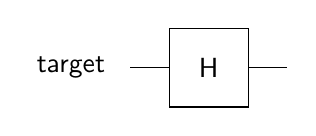
\begin{tikzpicture}[scale=.5] \node[draw=none] at (-3.5, 0) {target}; \draw (-2,0) -- (-1, 0); \draw (1, 0) -- (2, 0); \draw (-1,-1)--(-1,1)--(1,1)--(1,-1)--cycle; \node[draw=none] at (0, 0) {H}; \end{tikzpicture} } \] ~\newline
 
\begin{DoxyParams}[1]{Parameters}
\mbox{\tt in,out}  & {\em multi\+Qubit} & object representing the set of all qubits \\
\hline
\mbox{\tt in}  & {\em target\+Qubit} & qubit to operate on \\
\hline
\end{DoxyParams}

\begin{DoxyExceptions}{Exceptions}
{\em exit\+With\+Error} & if {\ttfamily target\+Qubit} is outside \mbox{[}0, {\ttfamily multi\+Qubit.\+num\+Qubits}). \\
\hline
\end{DoxyExceptions}


Definition at line 169 of file Qu\+E\+S\+T\+\_\+env\+\_\+local.\+c.



References Multi\+Qubit\+::chunk\+Id, chunk\+Is\+Upper(), exchange\+State\+Vectors(), get\+Chunk\+Pair\+Id(), hadamard\+Distributed(), hadamard\+Local(), half\+Matrix\+Block\+Fits\+In\+Chunk(), Multi\+Qubit\+::num\+Amps\+Per\+Chunk, Multi\+Qubit\+::num\+Qubits, Multi\+Qubit\+::pair\+State\+Vec, Qu\+E\+S\+T\+Assert(), R\+E\+AL, and Multi\+Qubit\+::state\+Vec.



Referenced by main(), and test\+\_\+hadamard().


\begin{DoxyCode}
170 \{
171     \mbox{\hyperlink{QuEST__env__local_8c_a3587b9d533e633ccf1abf9ad2ce45d8d}{QuESTAssert}}(targetQubit >= 0 && targetQubit < multiQubit.
      \mbox{\hyperlink{structMultiQubit_ab5b9795bdc6fb5855e1974dcbbaeb36f}{numQubits}}, 1, \_\_func\_\_);
172     \mbox{\hyperlink{QuEST_8c_aa9f0718b4dd794a3e1b143e3b153bfc5}{hadamardLocal}}(multiQubit, targetQubit);
173 \}
\end{DoxyCode}
\mbox{\Hypertarget{QuEST_8h_ae1b983b41249836ed2c2a81f77d83c40}\label{QuEST_8h_ae1b983b41249836ed2c2a81f77d83c40}} 
\index{Qu\+E\+S\+T.\+h@{Qu\+E\+S\+T.\+h}!init\+Classical\+State@{init\+Classical\+State}}
\index{init\+Classical\+State@{init\+Classical\+State}!Qu\+E\+S\+T.\+h@{Qu\+E\+S\+T.\+h}}
\paragraph{\texorpdfstring{init\+Classical\+State()}{initClassicalState()}}
{\footnotesize\ttfamily void init\+Classical\+State (\begin{DoxyParamCaption}\item[{\mbox{\hyperlink{structMultiQubit}{Multi\+Qubit}}}]{multi\+Qubit,  }\item[{long long int}]{state\+Ind }\end{DoxyParamCaption})}



Initialise a set of $ N $ qubits to the classical state with index {\ttfamily state\+Ind}. 

Note $ | 00 \dots 00 \rangle $ has {\ttfamily state\+Ind} 0, $ | 00 \dots 01 \rangle $ has {\ttfamily state\+Ind} 1, $ | 11 \dots 11 \rangle $ has {\ttfamily state\+Ind} $ 2^N - 1 $, etc. Subsequent calls to get\+Prob\+El will yield 0 for all indices except {\ttfamily state\+Ind}.


\begin{DoxyParams}[1]{Parameters}
\mbox{\tt in,out}  & {\em multi\+Qubit} & the object representing the set of qubits to be initialised \\
\hline
\mbox{\tt in}  & {\em state\+Ind} & the index (0 to the number of amplitudes, exclusive) of the state to give probability 1 \\
\hline
\end{DoxyParams}


Definition at line 222 of file Qu\+E\+S\+T.\+c.



References Multi\+Qubit\+::chunk\+Id, Multi\+Qubit\+::device\+State\+Vec, Complex\+Array\+::imag, Multi\+Qubit\+::num\+Amps\+Per\+Chunk, Complex\+Array\+::real, R\+E\+AL, and Multi\+Qubit\+::state\+Vec.



Referenced by test\+\_\+init\+Classical\+State().


\begin{DoxyCode}
223 \{
224     \textcolor{keywordtype}{long} \textcolor{keywordtype}{long} \textcolor{keywordtype}{int} stateVecSize;
225     \textcolor{keywordtype}{long} \textcolor{keywordtype}{long} \textcolor{keywordtype}{int} index;
226 
227     \textcolor{comment}{// dimension of the state vector}
228     stateVecSize = multiQubit.\mbox{\hyperlink{structMultiQubit_a1cad83601a78635dd278259c7ed54f18}{numAmpsPerChunk}};
229 
230     \textcolor{comment}{// Can't use multiQubit->stateVec as a private OMP var}
231     \mbox{\hyperlink{QuEST__precision_8h_a4b654506f18b8bfd61ad2a29a7e38c25}{REAL}} *stateVecReal = multiQubit.\mbox{\hyperlink{structMultiQubit_a45483190d6b01ef6b2f98f2bec9ab94f}{stateVec}}.\mbox{\hyperlink{structComplexArray_a4195cac6c784ea1b6271f1c7dba1548a}{real}};
232     \mbox{\hyperlink{QuEST__precision_8h_a4b654506f18b8bfd61ad2a29a7e38c25}{REAL}} *stateVecImag = multiQubit.\mbox{\hyperlink{structMultiQubit_a45483190d6b01ef6b2f98f2bec9ab94f}{stateVec}}.\mbox{\hyperlink{structComplexArray_a79dde47c7ae530c79cebfdf57b225968}{imag}};
233 
234     \textcolor{comment}{// initialise the state to |0000..0000>}
235 \textcolor{preprocessor}{# ifdef \_OPENMP}
236 \textcolor{preprocessor}{# pragma omp parallel \(\backslash\)}
237 \textcolor{preprocessor}{    default  (none) \(\backslash\)}
238 \textcolor{preprocessor}{    shared   (stateInd, stateVecSize, stateVecReal, stateVecImag) \(\backslash\)}
239 \textcolor{preprocessor}{    private  (index) }
240 \textcolor{preprocessor}{# endif}
241     \{
242 \textcolor{preprocessor}{# ifdef \_OPENMP}
243 \textcolor{preprocessor}{# pragma omp for schedule (static)}
244 \textcolor{preprocessor}{# endif}
245         \textcolor{keywordflow}{for} (index=0; index<stateVecSize; index++) \{
246             stateVecReal[index] = 0.0;
247             stateVecImag[index] = 0.0;
248         \}
249     \}
250 
251         \textcolor{comment}{// give the specified classical state prob 1}
252     \textcolor{keywordflow}{if} (multiQubit.\mbox{\hyperlink{structMultiQubit_ab10c88249fa3825d6227ceec01d37e37}{chunkId}} == stateInd/stateVecSize)\{
253         stateVecReal[stateInd % stateVecSize] = 1.0;
254         stateVecImag[stateInd % stateVecSize] = 0.0;
255     \}
256 \}
\end{DoxyCode}
\mbox{\Hypertarget{QuEST_8h_ad84a3ce68d1ca02b4e3f741ea45b6054}\label{QuEST_8h_ad84a3ce68d1ca02b4e3f741ea45b6054}} 
\index{Qu\+E\+S\+T.\+h@{Qu\+E\+S\+T.\+h}!init\+Qu\+E\+S\+T\+Env@{init\+Qu\+E\+S\+T\+Env}}
\index{init\+Qu\+E\+S\+T\+Env@{init\+Qu\+E\+S\+T\+Env}!Qu\+E\+S\+T.\+h@{Qu\+E\+S\+T.\+h}}
\paragraph{\texorpdfstring{init\+Qu\+E\+S\+T\+Env()}{initQuESTEnv()}}
{\footnotesize\ttfamily void init\+Qu\+E\+S\+T\+Env (\begin{DoxyParamCaption}\item[{\mbox{\hyperlink{structQuESTEnv}{Qu\+E\+S\+T\+Env}} $\ast$}]{env }\end{DoxyParamCaption})}



Initialize the Qu\+E\+ST environment. 

If something needs to be done to set up the execution environment, such as initializing M\+PI when running in distributed mode, it is handled here


\begin{DoxyParams}[1]{Parameters}
\mbox{\tt in,out}  & {\em env} & object representing the execution environment. A single instance is used for each program \\
\hline
\end{DoxyParams}


Definition at line 23 of file Qu\+E\+S\+T\+\_\+env\+\_\+local.\+c.



References env, G\+P\+U\+Exists(), Qu\+E\+S\+T\+Env\+::num\+Ranks, Qu\+E\+S\+T\+Env\+::rank, and seed\+Qu\+E\+S\+T\+Default().



Referenced by main().


\begin{DoxyCode}
23                                 \{
24     \textcolor{comment}{// init MPI environment}
25     \mbox{\hyperlink{runTests_8c_a5fd8ba97fcae3408ae6221dfc3cc1f93}{env}}->\mbox{\hyperlink{structQuESTEnv_aa648bb336cf8598467cb62db00b9cee8}{rank}}=0;
26     \mbox{\hyperlink{runTests_8c_a5fd8ba97fcae3408ae6221dfc3cc1f93}{env}}->\mbox{\hyperlink{structQuESTEnv_af22aacd7c9905accae28484785c193b4}{numRanks}}=1;
27         
28         \mbox{\hyperlink{QuEST_8c_ab0ab3ec70938712c26988a6aa51263a0}{seedQuESTDefault}}();
29 \}
\end{DoxyCode}
\mbox{\Hypertarget{QuEST_8h_af8a0082e2f695145bbfbb572e4c2e4f1}\label{QuEST_8h_af8a0082e2f695145bbfbb572e4c2e4f1}} 
\index{Qu\+E\+S\+T.\+h@{Qu\+E\+S\+T.\+h}!init\+State\+Plus@{init\+State\+Plus}}
\index{init\+State\+Plus@{init\+State\+Plus}!Qu\+E\+S\+T.\+h@{Qu\+E\+S\+T.\+h}}
\paragraph{\texorpdfstring{init\+State\+Plus()}{initStatePlus()}}
{\footnotesize\ttfamily void init\+State\+Plus (\begin{DoxyParamCaption}\item[{\mbox{\hyperlink{structMultiQubit}{Multi\+Qubit}}}]{multi\+Qubit }\end{DoxyParamCaption})}



Initialise a set of $ N $ qubits to the plus state $ {| + \rangle}^{\otimes N} = \frac{1}{\sqrt{2^N}} (| 0 \rangle + | 1 \rangle)^{\otimes N} $. 

This is the product state of $N$ qubits where every classical state is uniformly populated with real coefficient $\frac{1}{\sqrt{2^N}}$. This is equivalent to applying a Hadamard to every qubit in the zero state\+: $ \hat{H}^{\otimes N} {|0\rangle}^{\otimes N} $


\begin{DoxyParams}[1]{Parameters}
\mbox{\tt in,out}  & {\em multi\+Qubit} & the object representing the set of qubits to be initialised \\
\hline
\end{DoxyParams}


Definition at line 189 of file Qu\+E\+S\+T.\+c.



References Multi\+Qubit\+::device\+State\+Vec, Complex\+Array\+::imag, Multi\+Qubit\+::num\+Amps\+Per\+Chunk, Multi\+Qubit\+::num\+Chunks, Complex\+Array\+::real, R\+E\+AL, and Multi\+Qubit\+::state\+Vec.



Referenced by test\+\_\+collapse\+To\+Outcome(), test\+\_\+compact\+Unitary(), test\+\_\+find\+Probability\+Of\+Outcome(), test\+\_\+init\+State\+Plus(), test\+\_\+measure(), test\+\_\+measure\+With\+Stats(), and test\+\_\+unitary().


\begin{DoxyCode}
190 \{
191     \textcolor{keywordtype}{long} \textcolor{keywordtype}{long} \textcolor{keywordtype}{int} chunkSize, stateVecSize;
192     \textcolor{keywordtype}{long} \textcolor{keywordtype}{long} \textcolor{keywordtype}{int} index;
193 
194     \textcolor{comment}{// dimension of the state vector}
195     chunkSize = multiQubit.\mbox{\hyperlink{structMultiQubit_a1cad83601a78635dd278259c7ed54f18}{numAmpsPerChunk}};
196     stateVecSize = chunkSize*multiQubit.\mbox{\hyperlink{structMultiQubit_acd43f2f57991709c9e94f73662c972b2}{numChunks}};
197     \mbox{\hyperlink{QuEST__precision_8h_a4b654506f18b8bfd61ad2a29a7e38c25}{REAL}} normFactor = 1.0/sqrt((\mbox{\hyperlink{QuEST__precision_8h_a4b654506f18b8bfd61ad2a29a7e38c25}{REAL}})stateVecSize);
198 
199     \textcolor{comment}{// Can't use multiQubit->stateVec as a private OMP var}
200     \mbox{\hyperlink{QuEST__precision_8h_a4b654506f18b8bfd61ad2a29a7e38c25}{REAL}} *stateVecReal = multiQubit.\mbox{\hyperlink{structMultiQubit_a45483190d6b01ef6b2f98f2bec9ab94f}{stateVec}}.\mbox{\hyperlink{structComplexArray_a4195cac6c784ea1b6271f1c7dba1548a}{real}};
201     \mbox{\hyperlink{QuEST__precision_8h_a4b654506f18b8bfd61ad2a29a7e38c25}{REAL}} *stateVecImag = multiQubit.\mbox{\hyperlink{structMultiQubit_a45483190d6b01ef6b2f98f2bec9ab94f}{stateVec}}.\mbox{\hyperlink{structComplexArray_a79dde47c7ae530c79cebfdf57b225968}{imag}};
202 
203     \textcolor{comment}{// initialise the state to |0000..0000>}
204 \textcolor{preprocessor}{# ifdef \_OPENMP}
205 \textcolor{preprocessor}{# pragma omp parallel \(\backslash\)}
206 \textcolor{preprocessor}{    default  (none) \(\backslash\)}
207 \textcolor{preprocessor}{    shared   (chunkSize, stateVecReal, stateVecImag, normFactor) \(\backslash\)}
208 \textcolor{preprocessor}{    private  (index) }
209 \textcolor{preprocessor}{# endif}
210     \{
211 \textcolor{preprocessor}{# ifdef \_OPENMP}
212 \textcolor{preprocessor}{# pragma omp for schedule (static)}
213 \textcolor{preprocessor}{# endif}
214         \textcolor{keywordflow}{for} (index=0; index<chunkSize; index++) \{
215             stateVecReal[index] = normFactor;
216             stateVecImag[index] = 0.0;
217         \}
218     \}
219 \}
\end{DoxyCode}
\mbox{\Hypertarget{QuEST_8h_a9ba8171c9ec5c42202b144026527e9ec}\label{QuEST_8h_a9ba8171c9ec5c42202b144026527e9ec}} 
\index{Qu\+E\+S\+T.\+h@{Qu\+E\+S\+T.\+h}!init\+State\+Zero@{init\+State\+Zero}}
\index{init\+State\+Zero@{init\+State\+Zero}!Qu\+E\+S\+T.\+h@{Qu\+E\+S\+T.\+h}}
\paragraph{\texorpdfstring{init\+State\+Zero()}{initStateZero()}}
{\footnotesize\ttfamily void init\+State\+Zero (\begin{DoxyParamCaption}\item[{\mbox{\hyperlink{structMultiQubit}{Multi\+Qubit}}}]{multi\+Qubit }\end{DoxyParamCaption})}



Initialise a set of $ N $ qubits to the classical zero state $ {| 0 \rangle}^{\otimes N} $. 


\begin{DoxyParams}[1]{Parameters}
\mbox{\tt in,out}  & {\em multi\+Qubit} & the object representing the set of all qubits to initialise \\
\hline
\end{DoxyParams}


Definition at line 153 of file Qu\+E\+S\+T.\+c.



References Multi\+Qubit\+::chunk\+Id, Multi\+Qubit\+::device\+State\+Vec, Complex\+Array\+::imag, Multi\+Qubit\+::num\+Amps\+Per\+Chunk, Complex\+Array\+::real, R\+E\+AL, and Multi\+Qubit\+::state\+Vec.



Referenced by main(), test\+\_\+collapse\+To\+Outcome(), test\+\_\+find\+Probability\+Of\+Outcome(), test\+\_\+init\+State\+Zero(), test\+\_\+measure(), and test\+\_\+measure\+With\+Stats().


\begin{DoxyCode}
154 \{
155     \textcolor{keywordtype}{long} \textcolor{keywordtype}{long} \textcolor{keywordtype}{int} stateVecSize;
156     \textcolor{keywordtype}{long} \textcolor{keywordtype}{long} \textcolor{keywordtype}{int} index;
157 
158     \textcolor{comment}{// dimension of the state vector}
159     stateVecSize = multiQubit.\mbox{\hyperlink{structMultiQubit_a1cad83601a78635dd278259c7ed54f18}{numAmpsPerChunk}};
160 
161     \textcolor{comment}{// Can't use multiQubit->stateVec as a private OMP var}
162     \mbox{\hyperlink{QuEST__precision_8h_a4b654506f18b8bfd61ad2a29a7e38c25}{REAL}} *stateVecReal = multiQubit.\mbox{\hyperlink{structMultiQubit_a45483190d6b01ef6b2f98f2bec9ab94f}{stateVec}}.\mbox{\hyperlink{structComplexArray_a4195cac6c784ea1b6271f1c7dba1548a}{real}};
163     \mbox{\hyperlink{QuEST__precision_8h_a4b654506f18b8bfd61ad2a29a7e38c25}{REAL}} *stateVecImag = multiQubit.\mbox{\hyperlink{structMultiQubit_a45483190d6b01ef6b2f98f2bec9ab94f}{stateVec}}.\mbox{\hyperlink{structComplexArray_a79dde47c7ae530c79cebfdf57b225968}{imag}};
164 
165     \textcolor{comment}{// initialise the state to |0000..0000>}
166 \textcolor{preprocessor}{# ifdef \_OPENMP}
167 \textcolor{preprocessor}{# pragma omp parallel \(\backslash\)}
168 \textcolor{preprocessor}{    default  (none) \(\backslash\)}
169 \textcolor{preprocessor}{    shared   (stateVecSize, stateVecReal, stateVecImag) \(\backslash\)}
170 \textcolor{preprocessor}{    private  (index) }
171 \textcolor{preprocessor}{# endif}
172     \{
173 \textcolor{preprocessor}{# ifdef \_OPENMP}
174 \textcolor{preprocessor}{# pragma omp for schedule (static)}
175 \textcolor{preprocessor}{# endif}
176         \textcolor{keywordflow}{for} (index=0; index<stateVecSize; index++) \{
177             stateVecReal[index] = 0.0;
178             stateVecImag[index] = 0.0;
179         \}
180     \}
181 
182     \textcolor{keywordflow}{if} (multiQubit.\mbox{\hyperlink{structMultiQubit_ab10c88249fa3825d6227ceec01d37e37}{chunkId}}==0)\{
183         \textcolor{comment}{// zero state |0000..0000> has probability 1}
184         stateVecReal[0] = 1.0;
185         stateVecImag[0] = 0.0;
186     \}
187 \}
\end{DoxyCode}
\mbox{\Hypertarget{QuEST_8h_ad5774247d836267175c664cd0e451bcb}\label{QuEST_8h_ad5774247d836267175c664cd0e451bcb}} 
\index{Qu\+E\+S\+T.\+h@{Qu\+E\+S\+T.\+h}!measure@{measure}}
\index{measure@{measure}!Qu\+E\+S\+T.\+h@{Qu\+E\+S\+T.\+h}}
\paragraph{\texorpdfstring{measure()}{measure()}}
{\footnotesize\ttfamily int measure (\begin{DoxyParamCaption}\item[{\mbox{\hyperlink{structMultiQubit}{Multi\+Qubit}}}]{multi\+Qubit,  }\item[{int}]{measure\+Qubit }\end{DoxyParamCaption})}



Measures a single qubit, collapsing it randomly to 0 or 1. 

Outcome probabilities are weighted by the state vector, which is irreversibly changed after collapse to be consistent with the outcome.


\begin{DoxyParams}[1]{Parameters}
\mbox{\tt in,out}  & {\em multi\+Qubit} & object representing the set of all qubits \\
\hline
\mbox{\tt in}  & {\em measure\+Qubit} & qubit to measure \\
\hline
\end{DoxyParams}
\begin{DoxyReturn}{Returns}
the measurement outcome, 0 or 1 
\end{DoxyReturn}

\begin{DoxyExceptions}{Exceptions}
{\em exit\+With\+Error} & if {\ttfamily measure\+Qubit} is outside \mbox{[}0, {\ttfamily multi\+Qubit.\+num\+Qubits}) \\
\hline
\end{DoxyExceptions}


Definition at line 203 of file Qu\+E\+S\+T\+\_\+env\+\_\+local.\+c.



References measure\+With\+Stats(), Multi\+Qubit\+::num\+Qubits, Qu\+E\+S\+T\+Assert(), and R\+E\+AL.



Referenced by main(), and test\+\_\+measure().


\begin{DoxyCode}
203                                                     \{
204     \mbox{\hyperlink{QuEST__env__local_8c_a3587b9d533e633ccf1abf9ad2ce45d8d}{QuESTAssert}}(measureQubit >= 0 && measureQubit < multiQubit.
      \mbox{\hyperlink{structMultiQubit_ab5b9795bdc6fb5855e1974dcbbaeb36f}{numQubits}}, 2, \_\_func\_\_);
205     \mbox{\hyperlink{QuEST__precision_8h_a4b654506f18b8bfd61ad2a29a7e38c25}{REAL}} stateProb;
206     \textcolor{keywordflow}{return} \mbox{\hyperlink{QuEST__env__local_8c_a2ac46e470c750bf93c754e06c64b0a7a}{measureWithStats}}(multiQubit, measureQubit, &stateProb);
207 \}
\end{DoxyCode}
\mbox{\Hypertarget{QuEST_8h_a2ac46e470c750bf93c754e06c64b0a7a}\label{QuEST_8h_a2ac46e470c750bf93c754e06c64b0a7a}} 
\index{Qu\+E\+S\+T.\+h@{Qu\+E\+S\+T.\+h}!measure\+With\+Stats@{measure\+With\+Stats}}
\index{measure\+With\+Stats@{measure\+With\+Stats}!Qu\+E\+S\+T.\+h@{Qu\+E\+S\+T.\+h}}
\paragraph{\texorpdfstring{measure\+With\+Stats()}{measureWithStats()}}
{\footnotesize\ttfamily int measure\+With\+Stats (\begin{DoxyParamCaption}\item[{\mbox{\hyperlink{structMultiQubit}{Multi\+Qubit}}}]{multi\+Qubit,  }\item[{int}]{measure\+Qubit,  }\item[{\mbox{\hyperlink{QuEST__precision_8h_a4b654506f18b8bfd61ad2a29a7e38c25}{R\+E\+AL}} $\ast$}]{state\+Prob }\end{DoxyParamCaption})}



Measures a single qubit, collapsing it randomly to 0 or 1, and additionally gives the probability of that outcome. 

Outcome probabilities are weighted by the state vector, which is irreversibly changed after collapse to be consistent with the outcome.


\begin{DoxyParams}[1]{Parameters}
\mbox{\tt in,out}  & {\em multi\+Qubit} & object representing the set of all qubits \\
\hline
\mbox{\tt in}  & {\em measure\+Qubit} & qubit to measure \\
\hline
\mbox{\tt out}  & {\em state\+Prob} & a pointer to a R\+E\+AL which is set to the probability of the occurred outcome \\
\hline
\end{DoxyParams}
\begin{DoxyReturn}{Returns}
the measurement outcome, 0 or 1 
\end{DoxyReturn}

\begin{DoxyExceptions}{Exceptions}
{\em exit\+With\+Error} & if {\ttfamily measure\+Qubit} is outside \mbox{[}0, {\ttfamily multi\+Qubit.\+num\+Qubits}) \\
\hline
\end{DoxyExceptions}


Definition at line 209 of file Qu\+E\+S\+T\+\_\+env\+\_\+local.\+c.



References Multi\+Qubit\+::chunk\+Id, collapse\+To\+Outcome\+Distributed\+Renorm(), collapse\+To\+Outcome\+Distributed\+Set\+Zero(), collapse\+To\+Outcome\+Local(), find\+Probability\+Of\+Outcome(), genrand\+\_\+real1(), half\+Matrix\+Block\+Fits\+In\+Chunk(), is\+Chunk\+To\+Skip\+In\+Find\+P\+Zero(), Multi\+Qubit\+::num\+Amps\+Per\+Chunk, Multi\+Qubit\+::num\+Qubits, Qu\+E\+S\+T\+Assert(), R\+E\+AL, and R\+E\+A\+L\+\_\+\+E\+PS.



Referenced by main(), measure(), and test\+\_\+measure\+With\+Stats().


\begin{DoxyCode}
209                                                                               \{
210     \mbox{\hyperlink{QuEST__env__local_8c_a3587b9d533e633ccf1abf9ad2ce45d8d}{QuESTAssert}}(measureQubit >= 0 && measureQubit < multiQubit.
      \mbox{\hyperlink{structMultiQubit_ab5b9795bdc6fb5855e1974dcbbaeb36f}{numQubits}}, 2, \_\_func\_\_);
211 
212     \textcolor{keywordtype}{int} outcome;
213     \textcolor{comment}{// find probability of qubit being in state 1}
214     \mbox{\hyperlink{QuEST__precision_8h_a4b654506f18b8bfd61ad2a29a7e38c25}{REAL}} stateProbInternal = \mbox{\hyperlink{QuEST__env__local_8c_ad315c941a51bc053d39ebfa2040fd32e}{findProbabilityOfOutcome}}(multiQubit, measureQubit,
       1);
215 
216     \textcolor{comment}{// we can't collapse to a state that has a probability too close to zero}
217     \textcolor{keywordflow}{if} (stateProbInternal<\mbox{\hyperlink{QuEST__precision_8h_aebb5e6716e06431296af4d1a71744dec}{REAL\_EPS}}) outcome=0;
218     \textcolor{keywordflow}{else} \textcolor{keywordflow}{if} (1-stateProbInternal<\mbox{\hyperlink{QuEST__precision_8h_aebb5e6716e06431296af4d1a71744dec}{REAL\_EPS}}) outcome=1;
219     \textcolor{keywordflow}{else} \{
220         \textcolor{comment}{// ok. both P(0) and P(1) are large enough to resolve}
221         \textcolor{comment}{// generate random float on [0,1]}
222         \textcolor{keywordtype}{float} randNum = \mbox{\hyperlink{mt19937ar_8c_ac94ab75771800274ed1a2bedeca86f04}{genrand\_real1}}();
223         \textcolor{keywordflow}{if} (randNum<=stateProbInternal) outcome = 1;
224         \textcolor{keywordflow}{else} outcome = 0;
225     \} 
226     \textcolor{keywordflow}{if} (outcome==0) stateProbInternal = 1-stateProbInternal;
227     \mbox{\hyperlink{QuEST_8c_a01d9a8b7ff0e09ec399e158389783aa9}{collapseToOutcomeLocal}}(multiQubit, measureQubit, stateProbInternal, outcome);
228     *stateProb = stateProbInternal;
229     \textcolor{keywordflow}{return} outcome;
230 \}
\end{DoxyCode}
\mbox{\Hypertarget{QuEST_8h_afc1835c6b43b6e59ce7df7b13f274fc7}\label{QuEST_8h_afc1835c6b43b6e59ce7df7b13f274fc7}} 
\index{Qu\+E\+S\+T.\+h@{Qu\+E\+S\+T.\+h}!multi\+Controlled\+Phase\+Gate@{multi\+Controlled\+Phase\+Gate}}
\index{multi\+Controlled\+Phase\+Gate@{multi\+Controlled\+Phase\+Gate}!Qu\+E\+S\+T.\+h@{Qu\+E\+S\+T.\+h}}
\paragraph{\texorpdfstring{multi\+Controlled\+Phase\+Gate()}{multiControlledPhaseGate()}}
{\footnotesize\ttfamily void multi\+Controlled\+Phase\+Gate (\begin{DoxyParamCaption}\item[{\mbox{\hyperlink{structMultiQubit}{Multi\+Qubit}}}]{multi\+Qubit,  }\item[{int $\ast$}]{control\+Qubits,  }\item[{int}]{num\+Control\+Qubits }\end{DoxyParamCaption})}



Apply the multiple-\/qubit controlled phase gate, also known as the multiple-\/qubit controlled sigmaZ gate. 

For each state, if all control qubits have value one, multiply the amplitude of that state by -\/1. This applies the many-\/qubit unitary\+: \[ \begin{pmatrix} 1 \\ & 1 \\\ & & \ddots \\ & & & 1 \\ & & & & -1 \end{pmatrix} \] on the control qubits.

\[ \setlength{\fboxrule}{0.01pt} \fbox{ \begin{tikzpicture}[scale=.5] \node[draw=none] at (-3.5, 2) {controls}; \node[draw=none] at (0, 6) {$\vdots$}; \draw (0, 5) -- (0, 4); \draw (-2, 4) -- (2, 4); \draw[fill=black] (0, 4) circle (.2); \draw (0, 4) -- (0, 2); \draw (-2, 2) -- (2, 2); \draw[fill=black] (0, 2) circle (.2); \draw (0, 2) -- (0, 0); \draw (-2,0) -- (2, 0); \draw[fill=black] (0, 0) circle (.2); \end{tikzpicture} } \]


\begin{DoxyParams}[1]{Parameters}
\mbox{\tt in,out}  & {\em multi\+Qubit} & object representing the set of all qubits \\
\hline
\mbox{\tt in}  & {\em control\+Qubits} & array of input qubits \\
\hline
\mbox{\tt in}  & {\em num\+Control\+Qubits} & number of input qubits \\
\hline
\end{DoxyParams}

\begin{DoxyExceptions}{Exceptions}
{\em exit\+With\+Error} & if {\ttfamily num\+Control\+Qubits} is outside \mbox{[}1, {\ttfamily multi\+Qubit.\+num\+Qubits}) \\
\hline
\end{DoxyExceptions}


Definition at line 1783 of file Qu\+E\+S\+T.\+c.



References Multi\+Qubit\+::chunk\+Id, Complex\+Array\+::imag, Multi\+Qubit\+::num\+Amps\+Per\+Chunk, Multi\+Qubit\+::num\+Qubits, Qu\+E\+S\+T\+Assert(), Complex\+Array\+::real, R\+E\+AL, and Multi\+Qubit\+::state\+Vec.



Referenced by main(), and test\+\_\+multi\+Controlled\+Phase\+Gate().


\begin{DoxyCode}
1784 \{
1785     \textcolor{keywordtype}{long} \textcolor{keywordtype}{long} \textcolor{keywordtype}{int} index;
1786     \textcolor{keywordtype}{long} \textcolor{keywordtype}{long} \textcolor{keywordtype}{int} stateVecSize;
1787 
1788     \textcolor{keyword}{const} \textcolor{keywordtype}{long} \textcolor{keywordtype}{long} \textcolor{keywordtype}{int} chunkSize=multiQubit.\mbox{\hyperlink{structMultiQubit_a1cad83601a78635dd278259c7ed54f18}{numAmpsPerChunk}};
1789     \textcolor{keyword}{const} \textcolor{keywordtype}{long} \textcolor{keywordtype}{long} \textcolor{keywordtype}{int} chunkId=multiQubit.\mbox{\hyperlink{structMultiQubit_ab10c88249fa3825d6227ceec01d37e37}{chunkId}};
1790 
1791     \mbox{\hyperlink{QuEST__env__local_8c_a3587b9d533e633ccf1abf9ad2ce45d8d}{QuESTAssert}}(numControlQubits > 0 && numControlQubits <= multiQubit.
      \mbox{\hyperlink{structMultiQubit_ab5b9795bdc6fb5855e1974dcbbaeb36f}{numQubits}}, 4, \_\_func\_\_);
1792     \textcolor{keywordtype}{long} \textcolor{keywordtype}{long} \textcolor{keywordtype}{int} mask=0;
1793     \textcolor{keywordflow}{for} (\textcolor{keywordtype}{int} i=0; i<numControlQubits; i++) mask = mask | (1LL<<controlQubits[i]);
1794     \mbox{\hyperlink{QuEST__env__local_8c_a3587b9d533e633ccf1abf9ad2ce45d8d}{QuESTAssert}}(mask >=0 && mask <= (1LL<<multiQubit.\mbox{\hyperlink{structMultiQubit_ab5b9795bdc6fb5855e1974dcbbaeb36f}{numQubits}})-1, 2, \_\_func\_\_);
1795 
1796     stateVecSize = multiQubit.\mbox{\hyperlink{structMultiQubit_a1cad83601a78635dd278259c7ed54f18}{numAmpsPerChunk}};
1797     \mbox{\hyperlink{QuEST__precision_8h_a4b654506f18b8bfd61ad2a29a7e38c25}{REAL}} *stateVecReal = multiQubit.\mbox{\hyperlink{structMultiQubit_a45483190d6b01ef6b2f98f2bec9ab94f}{stateVec}}.\mbox{\hyperlink{structComplexArray_a4195cac6c784ea1b6271f1c7dba1548a}{real}};
1798     \mbox{\hyperlink{QuEST__precision_8h_a4b654506f18b8bfd61ad2a29a7e38c25}{REAL}} *stateVecImag = multiQubit.\mbox{\hyperlink{structMultiQubit_a45483190d6b01ef6b2f98f2bec9ab94f}{stateVec}}.\mbox{\hyperlink{structComplexArray_a79dde47c7ae530c79cebfdf57b225968}{imag}};
1799 
1800 \textcolor{preprocessor}{# ifdef \_OPENMP}
1801 \textcolor{preprocessor}{# pragma omp parallel \(\backslash\)}
1802 \textcolor{preprocessor}{    default  (none)                          \(\backslash\)}
1803 \textcolor{preprocessor}{    shared   (stateVecSize, stateVecReal,stateVecImag, mask ) \(\backslash\)}
1804 \textcolor{preprocessor}{    private  (index)}
1805 \textcolor{preprocessor}{# endif}
1806     \{
1807 \textcolor{preprocessor}{# ifdef \_OPENMP}
1808 \textcolor{preprocessor}{# pragma omp for schedule (static)}
1809 \textcolor{preprocessor}{# endif}
1810         \textcolor{keywordflow}{for} (index=0; index<stateVecSize; index++) \{
1811             \textcolor{keywordflow}{if} (mask == (mask & (index+chunkId*chunkSize)) )\{
1812                 stateVecReal [index] = - stateVecReal [index];
1813                 stateVecImag [index] = - stateVecImag [index];
1814             \}
1815         \}
1816     \}
1817 \}
\end{DoxyCode}
\mbox{\Hypertarget{QuEST_8h_ae395a79690283ed81106afadd7a8cd8a}\label{QuEST_8h_ae395a79690283ed81106afadd7a8cd8a}} 
\index{Qu\+E\+S\+T.\+h@{Qu\+E\+S\+T.\+h}!multi\+Controlled\+Unitary@{multi\+Controlled\+Unitary}}
\index{multi\+Controlled\+Unitary@{multi\+Controlled\+Unitary}!Qu\+E\+S\+T.\+h@{Qu\+E\+S\+T.\+h}}
\paragraph{\texorpdfstring{multi\+Controlled\+Unitary()}{multiControlledUnitary()}}
{\footnotesize\ttfamily void multi\+Controlled\+Unitary (\begin{DoxyParamCaption}\item[{\mbox{\hyperlink{structMultiQubit}{Multi\+Qubit}}}]{multi\+Qubit,  }\item[{int $\ast$}]{control\+Qubits,  }\item[{const int}]{num\+Control\+Qubits,  }\item[{const int}]{target\+Qubit,  }\item[{\mbox{\hyperlink{structComplexMatrix2}{Complex\+Matrix2}}}]{u }\end{DoxyParamCaption})}



Apply a general multiple-\/control single-\/target unitary, which can include a global phase factor. 

Any number of control qubits can be specified, and if all have value 1, the given unitary is applied to the target qubit. This effects the many-\/qubit unitary \[ \begin{pmatrix} 1 \\ & 1 \\\ & & \ddots \\ & & & u_{00} & u_{01}\\ & & & u_{10} & u_{11} \end{pmatrix} \] on the control and target qubits. The given 2x2 Complex\+Matrix must be unitary, otherwise an error is thrown.

\[ \setlength{\fboxrule}{0.01pt} \fbox{ 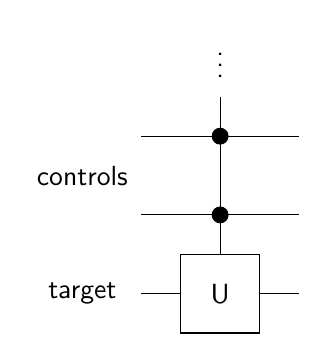
\begin{tikzpicture}[scale=.5] \node[draw=none] at (-3.5, 3) {controls}; \node[draw=none] at (-3.5, 0) {target}; \node[draw=none] at (0, 6) {$\vdots$}; \draw (0, 5) -- (0, 4); \draw (-2, 4) -- (2, 4); \draw[fill=black] (0, 4) circle (.2); \draw (0, 4) -- (0, 2); \draw (-2, 2) -- (2, 2); \draw[fill=black] (0, 2) circle (.2); \draw (0, 2) -- (0, 1); \draw (-2,0) -- (-1, 0); \draw (1, 0) -- (2, 0); \draw (-1,-1)--(-1,1)--(1,1)--(1,-1)--cycle; \node[draw=none] at (0, 0) {U}; \end{tikzpicture} } \]


\begin{DoxyParams}[1]{Parameters}
\mbox{\tt in,out}  & {\em multi\+Qubit} & object representing the set of all qubits \\
\hline
\mbox{\tt in}  & {\em control\+Qubits} & applies unitary if all qubits in this array equal 1 \\
\hline
\mbox{\tt in}  & {\em num\+Control\+Qubits} & number of control qubits \\
\hline
\mbox{\tt in}  & {\em target\+Qubit} & qubit to operate on \\
\hline
\mbox{\tt in}  & {\em u} & single-\/qubit unitary matrix to apply \\
\hline
\end{DoxyParams}

\begin{DoxyExceptions}{Exceptions}
{\em exit\+With\+Error} & if {\ttfamily num\+Control\+Qubits} is outside \mbox{[}1, {\ttfamily multi\+Qubit.\+num\+Qubits}\mbox{]}), or if any qubit index ({\ttfamily target\+Qubit} or one in {\ttfamily control\+Qubits}) is outside \mbox{[}0, {\ttfamily multi\+Qubit.\+num\+Qubits}\mbox{]}), or if {\ttfamily control\+Qubits} contains {\ttfamily target\+Qubit}, or if {\ttfamily u} is not unitary. \\
\hline
\end{DoxyExceptions}


Definition at line 137 of file Qu\+E\+S\+T\+\_\+env\+\_\+local.\+c.



References Multi\+Qubit\+::chunk\+Id, chunk\+Is\+Upper(), exchange\+State\+Vectors(), get\+Chunk\+Pair\+Id(), get\+Rot\+Angle\+From\+Unitary\+Matrix(), half\+Matrix\+Block\+Fits\+In\+Chunk(), multi\+Controlled\+Unitary\+Distributed(), multi\+Controlled\+Unitary\+Local(), Multi\+Qubit\+::num\+Amps\+Per\+Chunk, Multi\+Qubit\+::num\+Qubits, Multi\+Qubit\+::pair\+State\+Vec, Qu\+E\+S\+T\+Assert(), R\+E\+AL, Multi\+Qubit\+::state\+Vec, and validate\+Matrix\+Is\+Unitary().



Referenced by main(), and test\+\_\+multi\+Controlled\+Unitary().


\begin{DoxyCode}
138 \{
139     \mbox{\hyperlink{QuEST__env__local_8c_a3587b9d533e633ccf1abf9ad2ce45d8d}{QuESTAssert}}(targetQubit >= 0 && targetQubit < multiQubit.
      \mbox{\hyperlink{structMultiQubit_ab5b9795bdc6fb5855e1974dcbbaeb36f}{numQubits}}, 1, \_\_func\_\_);
140     \mbox{\hyperlink{QuEST__env__local_8c_a3587b9d533e633ccf1abf9ad2ce45d8d}{QuESTAssert}}(numControlQubits > 0 && numControlQubits <= multiQubit.
      \mbox{\hyperlink{structMultiQubit_ab5b9795bdc6fb5855e1974dcbbaeb36f}{numQubits}}, 4, \_\_func\_\_);
141     \mbox{\hyperlink{QuEST__env__local_8c_a3587b9d533e633ccf1abf9ad2ce45d8d}{QuESTAssert}}(\mbox{\hyperlink{QuEST_8c_ae4fea133d1a8f09ff8da03038100adb2}{validateMatrixIsUnitary}}(u), 5, \_\_func\_\_);
142 
143     \textcolor{keywordtype}{long} \textcolor{keywordtype}{long} \textcolor{keywordtype}{int} mask=0; 
144     \textcolor{keywordflow}{for} (\textcolor{keywordtype}{int} i=0; i<numControlQubits; i++) mask = mask | (1LL<<controlQubits[i]);
145     \mbox{\hyperlink{QuEST__env__local_8c_a3587b9d533e633ccf1abf9ad2ce45d8d}{QuESTAssert}}(mask >=0 && mask <= (1LL<<multiQubit.\mbox{\hyperlink{structMultiQubit_ab5b9795bdc6fb5855e1974dcbbaeb36f}{numQubits}})-1, 2, \_\_func\_\_);
146     \mbox{\hyperlink{QuEST__env__local_8c_a3587b9d533e633ccf1abf9ad2ce45d8d}{QuESTAssert}}((mask & (1LL<<targetQubit)) != (1LL<<targetQubit), 3, \_\_func\_\_);
147 
148     \mbox{\hyperlink{QuEST_8c_a1309eabcba3cb97fbc3cd2e606d17766}{multiControlledUnitaryLocal}}(multiQubit, targetQubit, mask, u);
149 \}
\end{DoxyCode}
\mbox{\Hypertarget{QuEST_8h_aa5e77e0e64f3a4a3d3f5cc7382bffcd9}\label{QuEST_8h_aa5e77e0e64f3a4a3d3f5cc7382bffcd9}} 
\index{Qu\+E\+S\+T.\+h@{Qu\+E\+S\+T.\+h}!report\+Multi\+Qubit\+Params@{report\+Multi\+Qubit\+Params}}
\index{report\+Multi\+Qubit\+Params@{report\+Multi\+Qubit\+Params}!Qu\+E\+S\+T.\+h@{Qu\+E\+S\+T.\+h}}
\paragraph{\texorpdfstring{report\+Multi\+Qubit\+Params()}{reportMultiQubitParams()}}
{\footnotesize\ttfamily void report\+Multi\+Qubit\+Params (\begin{DoxyParamCaption}\item[{\mbox{\hyperlink{structMultiQubit}{Multi\+Qubit}}}]{multi\+Qubit }\end{DoxyParamCaption})}



Report metainformation about a set of qubits\+: number of qubits, number of probability amplitudes. 


\begin{DoxyParams}[1]{Parameters}
\mbox{\tt in,out}  & {\em multi\+Qubit} & object representing the set of qubits \\
\hline
\mbox{\tt in}  & {\em env} & object representing the execution environment (local, multinode etc) \\
\hline
\end{DoxyParams}


Definition at line 125 of file Qu\+E\+S\+T.\+c.



References Multi\+Qubit\+::chunk\+Id, Multi\+Qubit\+::num\+Chunks, and Multi\+Qubit\+::num\+Qubits.



Referenced by main().


\begin{DoxyCode}
125                                                   \{
126     \textcolor{keywordtype}{long} \textcolor{keywordtype}{long} \textcolor{keywordtype}{int} numAmps = 1L << multiQubit.\mbox{\hyperlink{structMultiQubit_ab5b9795bdc6fb5855e1974dcbbaeb36f}{numQubits}};
127     \textcolor{keywordtype}{long} \textcolor{keywordtype}{long} \textcolor{keywordtype}{int} numAmpsPerRank = numAmps/multiQubit.\mbox{\hyperlink{structMultiQubit_acd43f2f57991709c9e94f73662c972b2}{numChunks}};
128     \textcolor{keywordflow}{if} (multiQubit.\mbox{\hyperlink{structMultiQubit_ab10c88249fa3825d6227ceec01d37e37}{chunkId}}==0)\{
129         printf(\textcolor{stringliteral}{"QUBITS:\(\backslash\)n"});
130         printf(\textcolor{stringliteral}{"Number of qubits is %d.\(\backslash\)n"}, multiQubit.\mbox{\hyperlink{structMultiQubit_ab5b9795bdc6fb5855e1974dcbbaeb36f}{numQubits}});
131         printf(\textcolor{stringliteral}{"Number of amps is %lld.\(\backslash\)n"}, numAmps);
132         printf(\textcolor{stringliteral}{"Number of amps per rank is %lld.\(\backslash\)n"}, numAmpsPerRank);
133     \}
134 \}
\end{DoxyCode}
\mbox{\Hypertarget{QuEST_8h_af8a14ae79c3fb2c0b5f6255cc37bebf9}\label{QuEST_8h_af8a14ae79c3fb2c0b5f6255cc37bebf9}} 
\index{Qu\+E\+S\+T.\+h@{Qu\+E\+S\+T.\+h}!report\+Qu\+E\+S\+T\+Env@{report\+Qu\+E\+S\+T\+Env}}
\index{report\+Qu\+E\+S\+T\+Env@{report\+Qu\+E\+S\+T\+Env}!Qu\+E\+S\+T.\+h@{Qu\+E\+S\+T.\+h}}
\paragraph{\texorpdfstring{report\+Qu\+E\+S\+T\+Env()}{reportQuESTEnv()}}
{\footnotesize\ttfamily void report\+Qu\+E\+S\+T\+Env (\begin{DoxyParamCaption}\item[{\mbox{\hyperlink{structQuESTEnv}{Qu\+E\+S\+T\+Env}}}]{env }\end{DoxyParamCaption})}



Report information about the Qu\+E\+ST environment. 


\begin{DoxyParams}[1]{Parameters}
\mbox{\tt in}  & {\em env} & object representing the execution environment. A single instance is used for each program \\
\hline
\end{DoxyParams}


Definition at line 43 of file Qu\+E\+S\+T\+\_\+env\+\_\+local.\+c.



References env, Qu\+E\+S\+T\+Env\+::num\+Ranks, Qu\+E\+S\+T\+Env\+::rank, and R\+E\+AL.



Referenced by main().


\begin{DoxyCode}
43                                  \{
44     printf(\textcolor{stringliteral}{"EXECUTION ENVIRONMENT:\(\backslash\)n"});
45     printf(\textcolor{stringliteral}{"Running locally on one node\(\backslash\)n"});
46     printf(\textcolor{stringliteral}{"Number of ranks is %d\(\backslash\)n"}, \mbox{\hyperlink{runTests_8c_a5fd8ba97fcae3408ae6221dfc3cc1f93}{env}}.\mbox{\hyperlink{structQuESTEnv_af22aacd7c9905accae28484785c193b4}{numRanks}});
47 \textcolor{preprocessor}{# ifdef \_OPENMP}
48     printf(\textcolor{stringliteral}{"OpenMP enabled\(\backslash\)n"});
49     printf(\textcolor{stringliteral}{"Number of threads available is %d\(\backslash\)n"}, omp\_get\_max\_threads());
50 \textcolor{preprocessor}{# else}
51     printf(\textcolor{stringliteral}{"OpenMP disabled\(\backslash\)n"});
52 \textcolor{preprocessor}{# endif}
53     printf(\textcolor{stringliteral}{"Precision: size of REAL is %ld bytes\(\backslash\)n"}, \textcolor{keyword}{sizeof}(\mbox{\hyperlink{QuEST__precision_8h_a4b654506f18b8bfd61ad2a29a7e38c25}{REAL}}));
54 \}
\end{DoxyCode}
\mbox{\Hypertarget{QuEST_8h_a96f4de9ce7fefc7680a44d601fc3d894}\label{QuEST_8h_a96f4de9ce7fefc7680a44d601fc3d894}} 
\index{Qu\+E\+S\+T.\+h@{Qu\+E\+S\+T.\+h}!report\+State@{report\+State}}
\index{report\+State@{report\+State}!Qu\+E\+S\+T.\+h@{Qu\+E\+S\+T.\+h}}
\paragraph{\texorpdfstring{report\+State()}{reportState()}}
{\footnotesize\ttfamily void report\+State (\begin{DoxyParamCaption}\item[{\mbox{\hyperlink{structMultiQubit}{Multi\+Qubit}}}]{multi\+Qubit }\end{DoxyParamCaption})}



Print the current state vector of probability amplitudes for a set of qubits to file. 

File format\+: \begin{DoxyVerb}real, imag
realComponent1, imagComponent1
realComponent2, imagComponent2
...
realComponentN, imagComponentN
\end{DoxyVerb}


File naming convention\+:

For each node that the program runs on, a file \textquotesingle{}state\+\_\+rank\+\_\+\mbox{[}node\+\_\+rank\mbox{]}.csv\textquotesingle{} is generated. If there is more than one node, ranks after the first do not include the header \begin{DoxyVerb}real, imag
\end{DoxyVerb}
 so that files are easier to combine.


\begin{DoxyParams}[1]{Parameters}
\mbox{\tt in,out}  & {\em multi\+Qubit} & object representing the set of qubits \\
\hline
\end{DoxyParams}


Definition at line 86 of file Qu\+E\+S\+T.\+c.



References Multi\+Qubit\+::chunk\+Id, Complex\+Array\+::imag, Multi\+Qubit\+::num\+Amps\+Per\+Chunk, Qu\+E\+S\+T\+Assert(), Complex\+Array\+::real, R\+E\+A\+L\+\_\+\+S\+T\+R\+I\+N\+G\+\_\+\+F\+O\+R\+M\+AT, and Multi\+Qubit\+::state\+Vec.


\begin{DoxyCode}
86                                        \{
87     FILE *state;
88     \textcolor{keywordtype}{char} filename[100];
89     \textcolor{keywordtype}{long} \textcolor{keywordtype}{long} \textcolor{keywordtype}{int} index;
90     sprintf(filename, \textcolor{stringliteral}{"state\_rank\_%d.csv"}, multiQubit.\mbox{\hyperlink{structMultiQubit_ab10c88249fa3825d6227ceec01d37e37}{chunkId}});
91     state = fopen(filename, \textcolor{stringliteral}{"w"});
92     \mbox{\hyperlink{QuEST__env__local_8c_a3587b9d533e633ccf1abf9ad2ce45d8d}{QuESTAssert}}(state!=NULL, 11, \_\_func\_\_);
93     \textcolor{keywordflow}{if} (multiQubit.\mbox{\hyperlink{structMultiQubit_ab10c88249fa3825d6227ceec01d37e37}{chunkId}}==0) fprintf(state, \textcolor{stringliteral}{"real, imag\(\backslash\)n"});
94 
95     \textcolor{keywordflow}{for}(index=0; index<multiQubit.\mbox{\hyperlink{structMultiQubit_a1cad83601a78635dd278259c7ed54f18}{numAmpsPerChunk}}; index++)\{
96         fprintf(state, \mbox{\hyperlink{QuEST__precision_8h_ad751ac7ddc8ec19f23fb33083c0da8da}{REAL\_STRING\_FORMAT}} \textcolor{stringliteral}{","} 
      \mbox{\hyperlink{QuEST__precision_8h_ad751ac7ddc8ec19f23fb33083c0da8da}{REAL\_STRING\_FORMAT}} \textcolor{stringliteral}{"\(\backslash\)n"}, multiQubit.\mbox{\hyperlink{structMultiQubit_a45483190d6b01ef6b2f98f2bec9ab94f}{stateVec}}.\mbox{\hyperlink{structComplexArray_a4195cac6c784ea1b6271f1c7dba1548a}{real}}[index], multiQubit.
      \mbox{\hyperlink{structMultiQubit_a45483190d6b01ef6b2f98f2bec9ab94f}{stateVec}}.\mbox{\hyperlink{structComplexArray_a79dde47c7ae530c79cebfdf57b225968}{imag}}[index]);
97     \}
98     fclose(state);
99 \}
\end{DoxyCode}
\mbox{\Hypertarget{QuEST_8h_a842d6884e063a5865a2232cba56b65ac}\label{QuEST_8h_a842d6884e063a5865a2232cba56b65ac}} 
\index{Qu\+E\+S\+T.\+h@{Qu\+E\+S\+T.\+h}!report\+State\+To\+Screen@{report\+State\+To\+Screen}}
\index{report\+State\+To\+Screen@{report\+State\+To\+Screen}!Qu\+E\+S\+T.\+h@{Qu\+E\+S\+T.\+h}}
\paragraph{\texorpdfstring{report\+State\+To\+Screen()}{reportStateToScreen()}}
{\footnotesize\ttfamily void report\+State\+To\+Screen (\begin{DoxyParamCaption}\item[{\mbox{\hyperlink{structMultiQubit}{Multi\+Qubit}}}]{multi\+Qubit,  }\item[{\mbox{\hyperlink{structQuESTEnv}{Qu\+E\+S\+T\+Env}}}]{env,  }\item[{int}]{report\+Rank }\end{DoxyParamCaption})}



Print the current state vector of probability amplitudes for a set of qubits to standard out. 

For debugging purposes. Each rank should print output serially. Only print output for systems $<$= 5 qubits 

Definition at line 101 of file Qu\+E\+S\+T.\+c.



References Multi\+Qubit\+::chunk\+Id, copy\+State\+From\+G\+P\+U(), env, Complex\+Array\+::imag, Multi\+Qubit\+::num\+Amps\+Per\+Chunk, Multi\+Qubit\+::num\+Chunks, Multi\+Qubit\+::num\+Qubits, Complex\+Array\+::real, R\+E\+A\+L\+\_\+\+S\+T\+R\+I\+N\+G\+\_\+\+F\+O\+R\+M\+AT, Multi\+Qubit\+::state\+Vec, and sync\+Qu\+E\+S\+T\+Env().



Referenced by report\+Test().


\begin{DoxyCode}
101                                                                              \{
102     \textcolor{keywordtype}{long} \textcolor{keywordtype}{long} \textcolor{keywordtype}{int} index;
103     \textcolor{keywordtype}{int} rank;
104     \textcolor{keywordflow}{if} (multiQubit.\mbox{\hyperlink{structMultiQubit_ab5b9795bdc6fb5855e1974dcbbaeb36f}{numQubits}}<=5)\{
105         \textcolor{keywordflow}{for} (rank=0; rank<multiQubit.\mbox{\hyperlink{structMultiQubit_acd43f2f57991709c9e94f73662c972b2}{numChunks}}; rank++)\{
106             \textcolor{keywordflow}{if} (multiQubit.\mbox{\hyperlink{structMultiQubit_ab10c88249fa3825d6227ceec01d37e37}{chunkId}}==rank)\{
107                 \textcolor{keywordflow}{if} (reportRank) \{
108                     printf(\textcolor{stringliteral}{"Reporting state from rank %d [\(\backslash\)n"}, multiQubit.
      \mbox{\hyperlink{structMultiQubit_ab10c88249fa3825d6227ceec01d37e37}{chunkId}});
109                     printf(\textcolor{stringliteral}{"real, imag\(\backslash\)n"});
110                 \} \textcolor{keywordflow}{else} \textcolor{keywordflow}{if} (rank==0) \{
111                     printf(\textcolor{stringliteral}{"Reporting state [\(\backslash\)n"});
112                     printf(\textcolor{stringliteral}{"real, imag\(\backslash\)n"});
113                 \}
114 
115                 \textcolor{keywordflow}{for}(index=0; index<multiQubit.\mbox{\hyperlink{structMultiQubit_a1cad83601a78635dd278259c7ed54f18}{numAmpsPerChunk}}; index++)\{
116                     printf(\mbox{\hyperlink{QuEST__precision_8h_ad751ac7ddc8ec19f23fb33083c0da8da}{REAL\_STRING\_FORMAT}} \textcolor{stringliteral}{", "} 
      \mbox{\hyperlink{QuEST__precision_8h_ad751ac7ddc8ec19f23fb33083c0da8da}{REAL\_STRING\_FORMAT}} \textcolor{stringliteral}{"\(\backslash\)n"}, multiQubit.\mbox{\hyperlink{structMultiQubit_a45483190d6b01ef6b2f98f2bec9ab94f}{stateVec}}.\mbox{\hyperlink{structComplexArray_a4195cac6c784ea1b6271f1c7dba1548a}{real}}[index], multiQubit.
      \mbox{\hyperlink{structMultiQubit_a45483190d6b01ef6b2f98f2bec9ab94f}{stateVec}}.\mbox{\hyperlink{structComplexArray_a79dde47c7ae530c79cebfdf57b225968}{imag}}[index]);
117                 \}
118                 \textcolor{keywordflow}{if} (reportRank || rank==multiQubit.\mbox{\hyperlink{structMultiQubit_acd43f2f57991709c9e94f73662c972b2}{numChunks}}-1) printf(\textcolor{stringliteral}{"]\(\backslash\)n"});
119             \}
120             \mbox{\hyperlink{QuEST__env__local_8c_a8d31fe2d1ad4d01e2a1f5f6b8bc15b77}{syncQuESTEnv}}(\mbox{\hyperlink{runTests_8c_a5fd8ba97fcae3408ae6221dfc3cc1f93}{env}});
121         \}
122     \} \textcolor{keywordflow}{else} printf(\textcolor{stringliteral}{"Error: reportStateToScreen will not print output for systems of more than 5 qubits.\(\backslash\)n"});
123 \}
\end{DoxyCode}
\mbox{\Hypertarget{QuEST_8h_a8810423457803005fecd415f4299f40d}\label{QuEST_8h_a8810423457803005fecd415f4299f40d}} 
\index{Qu\+E\+S\+T.\+h@{Qu\+E\+S\+T.\+h}!rotate\+Around\+Axis@{rotate\+Around\+Axis}}
\index{rotate\+Around\+Axis@{rotate\+Around\+Axis}!Qu\+E\+S\+T.\+h@{Qu\+E\+S\+T.\+h}}
\paragraph{\texorpdfstring{rotate\+Around\+Axis()}{rotateAroundAxis()}}
{\footnotesize\ttfamily void rotate\+Around\+Axis (\begin{DoxyParamCaption}\item[{\mbox{\hyperlink{structMultiQubit}{Multi\+Qubit}}}]{multi\+Qubit,  }\item[{const int}]{rot\+Qubit,  }\item[{\mbox{\hyperlink{QuEST__precision_8h_a4b654506f18b8bfd61ad2a29a7e38c25}{R\+E\+AL}}}]{angle,  }\item[{\mbox{\hyperlink{structVector}{Vector}}}]{axis }\end{DoxyParamCaption})}



Rotate a single qubit by a given angle around a given vector on the Bloch-\/sphere. 

The vector must not be zero (else an error is thrown), but needn\textquotesingle{}t be unit magnitude.

For angle $\theta$ and axis vector $\vec{n}$, applies $R_{\hat{n}} = \exp \left(- i \frac{\theta}{2} \hat{n} \cdot \vec{\sigma} \right) $ where $\vec{\sigma}$ is the vector of Pauli matrices.


\begin{DoxyParams}[1]{Parameters}
\mbox{\tt in,out}  & {\em multi\+Qubit} & object representing the set of all qubits \\
\hline
\mbox{\tt in}  & {\em rot\+Qubit} & qubit to rotate \\
\hline
\mbox{\tt in}  & {\em angle} & angle by which to rotate in radians \\
\hline
\mbox{\tt in}  & {\em axis} & vector around which to rotate (can be non-\/unit; will be normalised) \\
\hline
\end{DoxyParams}

\begin{DoxyExceptions}{Exceptions}
{\em exit\+With\+Error} & if {\ttfamily rot\+Qubit} is outside \mbox{[}0, {\ttfamily multi\+Qubit.\+num\+Qubits}), or if {\ttfamily axis} is the zero vector \\
\hline
\end{DoxyExceptions}


Definition at line 428 of file Qu\+E\+S\+T.\+c.



References compact\+Unitary(), Complex\+::imag, Complex\+::real, Vector\+::x, Vector\+::y, and Vector\+::z.



Referenced by main(), rotate\+X(), rotate\+Y(), and rotate\+Z().


\begin{DoxyCode}
428                                                                                          \{
429 
430     \textcolor{keywordtype}{double} mag = sqrt(pow(axis.\mbox{\hyperlink{structVector_aac7abe171ba4bada50ed72acba6259fc}{x}},2) + pow(axis.\mbox{\hyperlink{structVector_a375ca805d4c808a53d7c4e0c737ae3de}{y}},2) + pow(axis.\mbox{\hyperlink{structVector_ad4e863651be7d6b7e2b28cd7445a0ccf}{z}},2));
431     \mbox{\hyperlink{structVector}{Vector}} unitAxis = \{axis.\mbox{\hyperlink{structVector_aac7abe171ba4bada50ed72acba6259fc}{x}}/mag, axis.\mbox{\hyperlink{structVector_a375ca805d4c808a53d7c4e0c737ae3de}{y}}/mag, axis.\mbox{\hyperlink{structVector_ad4e863651be7d6b7e2b28cd7445a0ccf}{z}}/mag\};
432 
433     \mbox{\hyperlink{structComplex}{Complex}} alpha, beta;
434     alpha.\mbox{\hyperlink{structComplex_a479ad939835457595fcca3ca55c06283}{real}} = cos(angle/2.0);
435     alpha.\mbox{\hyperlink{structComplex_a1151948284b21c0052f203f23ab931d9}{imag}} = -sin(angle/2.0)*unitAxis.\mbox{\hyperlink{structVector_ad4e863651be7d6b7e2b28cd7445a0ccf}{z}};       
436     beta.\mbox{\hyperlink{structComplex_a479ad939835457595fcca3ca55c06283}{real}} = sin(angle/2.0)*unitAxis.\mbox{\hyperlink{structVector_a375ca805d4c808a53d7c4e0c737ae3de}{y}};
437     beta.\mbox{\hyperlink{structComplex_a1151948284b21c0052f203f23ab931d9}{imag}} = -sin(angle/2.0)*unitAxis.\mbox{\hyperlink{structVector_aac7abe171ba4bada50ed72acba6259fc}{x}};
438     \mbox{\hyperlink{QuEST__env__local_8c_a03b13dfcabd8c59b50dbdd3af44ba8b2}{compactUnitary}}(multiQubit, rotQubit, alpha, beta);
439 \}
\end{DoxyCode}
\mbox{\Hypertarget{QuEST_8h_a6cc7fa705a2f2e6b486b49c5589d5df5}\label{QuEST_8h_a6cc7fa705a2f2e6b486b49c5589d5df5}} 
\index{Qu\+E\+S\+T.\+h@{Qu\+E\+S\+T.\+h}!rotateX@{rotateX}}
\index{rotateX@{rotateX}!Qu\+E\+S\+T.\+h@{Qu\+E\+S\+T.\+h}}
\paragraph{\texorpdfstring{rotate\+X()}{rotateX()}}
{\footnotesize\ttfamily void rotateX (\begin{DoxyParamCaption}\item[{\mbox{\hyperlink{structMultiQubit}{Multi\+Qubit}}}]{multi\+Qubit,  }\item[{const int}]{rot\+Qubit,  }\item[{\mbox{\hyperlink{QuEST__precision_8h_a4b654506f18b8bfd61ad2a29a7e38c25}{R\+E\+AL}}}]{angle }\end{DoxyParamCaption})}



Rotate a single qubit by a given angle around the X-\/axis of the Bloch-\/sphere. 

For angle $\theta$, applies \[ \begin{pmatrix} \cos\theta/2 & -i \sin \theta/2\\ -i \sin \theta/2 & \cos \theta/2 \end{pmatrix} \]

\[ \setlength{\fboxrule}{0.01pt} \fbox{ 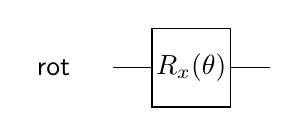
\begin{tikzpicture}[scale=.5] \node[draw=none] at (-3.5, 0) {rot}; \draw (-2,0) -- (-1, 0); \draw (1, 0) -- (2, 0); \draw (-1,-1)--(-1,1)--(1,1)--(1,-1)--cycle; \node[draw=none] at (0, 0) {$R_x(\theta)$}; \end{tikzpicture} } \]


\begin{DoxyParams}[1]{Parameters}
\mbox{\tt in,out}  & {\em multi\+Qubit} & object representing the set of all qubits \\
\hline
\mbox{\tt in}  & {\em rot\+Qubit} & qubit to rotate \\
\hline
\mbox{\tt in}  & {\em angle} & angle by which to rotate in radians \\
\hline
\end{DoxyParams}

\begin{DoxyExceptions}{Exceptions}
{\em exit\+With\+Error} & if {\ttfamily rot\+Qubit} is outside \mbox{[}0, {\ttfamily multi\+Qubit.\+num\+Qubits}). \\
\hline
\end{DoxyExceptions}


Definition at line 441 of file Qu\+E\+S\+T.\+c.



References rotate\+Around\+Axis().


\begin{DoxyCode}
441                                                                    \{
442 
443     \mbox{\hyperlink{structVector}{Vector}} unitAxis = \{1, 0, 0\};
444     \mbox{\hyperlink{QuEST_8c_a8810423457803005fecd415f4299f40d}{rotateAroundAxis}}(multiQubit, rotQubit, angle, unitAxis);
445 \}
\end{DoxyCode}
\mbox{\Hypertarget{QuEST_8h_ace0d3592d38a990e81a434c4e9681500}\label{QuEST_8h_ace0d3592d38a990e81a434c4e9681500}} 
\index{Qu\+E\+S\+T.\+h@{Qu\+E\+S\+T.\+h}!rotateY@{rotateY}}
\index{rotateY@{rotateY}!Qu\+E\+S\+T.\+h@{Qu\+E\+S\+T.\+h}}
\paragraph{\texorpdfstring{rotate\+Y()}{rotateY()}}
{\footnotesize\ttfamily void rotateY (\begin{DoxyParamCaption}\item[{\mbox{\hyperlink{structMultiQubit}{Multi\+Qubit}}}]{multi\+Qubit,  }\item[{const int}]{rot\+Qubit,  }\item[{\mbox{\hyperlink{QuEST__precision_8h_a4b654506f18b8bfd61ad2a29a7e38c25}{R\+E\+AL}}}]{angle }\end{DoxyParamCaption})}



Rotate a single qubit by a given angle around the Y-\/axis of the Bloch-\/sphere. 

For angle $\theta$, applies \[ \begin{pmatrix} \cos\theta/2 & - \sin \theta/2\\ \sin \theta/2 & \cos \theta/2 \end{pmatrix} \] ~\newline
 \[ \setlength{\fboxrule}{0.01pt} \fbox{ 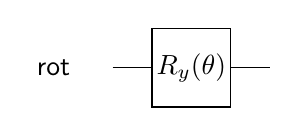
\begin{tikzpicture}[scale=.5] \node[draw=none] at (-3.5, 0) {rot}; \draw (-2,0) -- (-1, 0); \draw (1, 0) -- (2, 0); \draw (-1,-1)--(-1,1)--(1,1)--(1,-1)--cycle; \node[draw=none] at (0, 0) {$R_y(\theta)$}; \end{tikzpicture} } \]


\begin{DoxyParams}[1]{Parameters}
\mbox{\tt in,out}  & {\em multi\+Qubit} & object representing the set of all qubits \\
\hline
\mbox{\tt in}  & {\em rot\+Qubit} & qubit to rotate \\
\hline
\mbox{\tt in}  & {\em angle} & angle by which to rotate in radians \\
\hline
\end{DoxyParams}

\begin{DoxyExceptions}{Exceptions}
{\em exit\+With\+Error} & if {\ttfamily rot\+Qubit} is outside \mbox{[}0, {\ttfamily multi\+Qubit.\+num\+Qubits}). \\
\hline
\end{DoxyExceptions}


Definition at line 447 of file Qu\+E\+S\+T.\+c.



References rotate\+Around\+Axis().



Referenced by main().


\begin{DoxyCode}
447                                                                    \{
448 
449     \mbox{\hyperlink{structVector}{Vector}} unitAxis = \{0, 1, 0\};
450     \mbox{\hyperlink{QuEST_8c_a8810423457803005fecd415f4299f40d}{rotateAroundAxis}}(multiQubit, rotQubit, angle, unitAxis);
451 \}
\end{DoxyCode}
\mbox{\Hypertarget{QuEST_8h_abd621412ad30c1b034f4ce153c4afe10}\label{QuEST_8h_abd621412ad30c1b034f4ce153c4afe10}} 
\index{Qu\+E\+S\+T.\+h@{Qu\+E\+S\+T.\+h}!rotateZ@{rotateZ}}
\index{rotateZ@{rotateZ}!Qu\+E\+S\+T.\+h@{Qu\+E\+S\+T.\+h}}
\paragraph{\texorpdfstring{rotate\+Z()}{rotateZ()}}
{\footnotesize\ttfamily void rotateZ (\begin{DoxyParamCaption}\item[{\mbox{\hyperlink{structMultiQubit}{Multi\+Qubit}}}]{multi\+Qubit,  }\item[{const int}]{rot\+Qubit,  }\item[{\mbox{\hyperlink{QuEST__precision_8h_a4b654506f18b8bfd61ad2a29a7e38c25}{R\+E\+AL}}}]{angle }\end{DoxyParamCaption})}



Rotate a single qubit by a given angle around the Z-\/axis of the Bloch-\/sphere (also known as a phase shift gate). 

For angle $\theta$, applies \[ \begin{pmatrix} \exp(-i \theta/2) & 0 \\ 0 & \exp(i \theta/2) \end{pmatrix} \]

\[ \setlength{\fboxrule}{0.01pt} \fbox{ 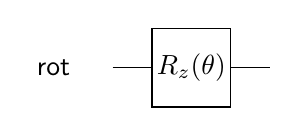
\begin{tikzpicture}[scale=.5] \node[draw=none] at (-3.5, 0) {rot}; \draw (-2,0) -- (-1, 0); \draw (1, 0) -- (2, 0); \draw (-1,-1)--(-1,1)--(1,1)--(1,-1)--cycle; \node[draw=none] at (0, 0) {$R_z(\theta)$}; \end{tikzpicture} } \]


\begin{DoxyParams}[1]{Parameters}
\mbox{\tt in,out}  & {\em multi\+Qubit} & object representing the set of all qubits \\
\hline
\mbox{\tt in}  & {\em rot\+Qubit} & qubit to rotate \\
\hline
\mbox{\tt in}  & {\em angle} & angle by which to rotate in radians \\
\hline
\end{DoxyParams}

\begin{DoxyExceptions}{Exceptions}
{\em exit\+With\+Error} & if {\ttfamily rot\+Qubit} is outside \mbox{[}0, {\ttfamily multi\+Qubit.\+num\+Qubits}). \\
\hline
\end{DoxyExceptions}


Definition at line 453 of file Qu\+E\+S\+T.\+c.



References rotate\+Around\+Axis().


\begin{DoxyCode}
453                                                                    \{
454 
455     \mbox{\hyperlink{structVector}{Vector}} unitAxis = \{0, 0, 1\};
456     \mbox{\hyperlink{QuEST_8c_a8810423457803005fecd415f4299f40d}{rotateAroundAxis}}(multiQubit, rotQubit, angle, unitAxis);
457 \}
\end{DoxyCode}
\mbox{\Hypertarget{QuEST_8h_a95012dad46509b4b461974c34cfd7b3d}\label{QuEST_8h_a95012dad46509b4b461974c34cfd7b3d}} 
\index{Qu\+E\+S\+T.\+h@{Qu\+E\+S\+T.\+h}!seed\+Qu\+E\+ST@{seed\+Qu\+E\+ST}}
\index{seed\+Qu\+E\+ST@{seed\+Qu\+E\+ST}!Qu\+E\+S\+T.\+h@{Qu\+E\+S\+T.\+h}}
\paragraph{\texorpdfstring{seed\+Qu\+E\+S\+T()}{seedQuEST()}}
{\footnotesize\ttfamily void seed\+Qu\+E\+ST (\begin{DoxyParamCaption}\item[{unsigned long int $\ast$}]{seed\+Array,  }\item[{int}]{num\+Seeds }\end{DoxyParamCaption})}



Seed the Mersenne Twister used for random number generation in the Qu\+E\+ST environment with a user defined seed. 

This function uses the mt19937 init\+\_\+by\+\_\+array function with num\+Seeds keys supplied by the user. Subsequent calls to mt19937 genrand functions will use this seeding. For a multi process code, the same seed is given to all process, therefore this seeding is only appropriate to use for functions such as measure where all processes require the same random value.


\begin{DoxyParams}[1]{Parameters}
\mbox{\tt in}  & {\em seed\+Array} & Array of integers to use as seed. This allows the MT to be initialised with more than a 32-\/bit integer if required \\
\hline
\mbox{\tt in}  & {\em num\+Seeds} & Length of seed\+Array\\
\hline
\end{DoxyParams}
For more information about the MT, see \href{http://www.math.sci.hiroshima-u.ac.jp/~m-mat/MT/MT2002/emt19937ar.html}{\tt http\+://www.\+math.\+sci.\+hiroshima-\/u.\+ac.\+jp/$\sim$m-\/mat/\+M\+T/\+M\+T2002/emt19937ar.\+html}

Seed the Mersenne Twister used for random number generation in the Qu\+E\+ST environment with a user defined seed. 

Definition at line 2019 of file Qu\+E\+S\+T.\+c.



References init\+\_\+by\+\_\+array().



Referenced by test\+\_\+measure().


\begin{DoxyCode}
2019                                                           \{
2020     \textcolor{comment}{// init MT random number generator with user defined list of seeds}
2021     \textcolor{comment}{// for the MPI version, it is ok that all procs will get the same seed as random numbers will only be }
2022     \textcolor{comment}{// used by the master process}
2023     \mbox{\hyperlink{mt19937ar_8c_ac1283f9b1ed571332f5ffe53545ffc16}{init\_by\_array}}(seedArray, numSeeds); 
2024 \}
\end{DoxyCode}
\mbox{\Hypertarget{QuEST_8h_aa8437ef3bf135231e2916e64dde1c94e}\label{QuEST_8h_aa8437ef3bf135231e2916e64dde1c94e}} 
\index{Qu\+E\+S\+T.\+h@{Qu\+E\+S\+T.\+h}!seed\+Qu\+E\+S\+T\+Default@{seed\+Qu\+E\+S\+T\+Default}}
\index{seed\+Qu\+E\+S\+T\+Default@{seed\+Qu\+E\+S\+T\+Default}!Qu\+E\+S\+T.\+h@{Qu\+E\+S\+T.\+h}}
\paragraph{\texorpdfstring{seed\+Qu\+E\+S\+T\+Default()}{seedQuESTDefault()}}
{\footnotesize\ttfamily void seed\+Qu\+E\+S\+T\+Default (\begin{DoxyParamCaption}\item[{void}]{ }\end{DoxyParamCaption})}



Seed the Mersenne Twister used for random number generation in the Qu\+E\+ST environment with an example defualt seed. 

This default seeding function uses the mt19937 init\+\_\+by\+\_\+array function with three keys -- time, pid and hostname. Subsequent calls to mt19937 genrand functions will use this seeding. For a multi process code, the same seed is given to all process, therefore this seeding is only appropriate to use for functions such as measure where all processes require the same random value.

For more information about the MT, see \href{http://www.math.sci.hiroshima-u.ac.jp/~m-mat/MT/MT2002/emt19937ar.html}{\tt http\+://www.\+math.\+sci.\+hiroshima-\/u.\+ac.\+jp/$\sim$m-\/mat/\+M\+T/\+M\+T2002/emt19937ar.\+html} 

Definition at line 1994 of file Qu\+E\+S\+T.\+c.



References hash\+String(), and init\+\_\+by\+\_\+array().



Referenced by init\+Qu\+E\+S\+T\+Env().


\begin{DoxyCode}
1994                        \{
1995     \textcolor{comment}{// init MT random number generator with three keys -- time, pid and a hash of hostname }
1996     \textcolor{comment}{// for the MPI version, it is ok that all procs will get the same seed as random numbers will only be }
1997     \textcolor{comment}{// used by the master process}
1998 
1999     \textcolor{keyword}{struct }timeval  tv;
2000     gettimeofday(&tv, NULL);
2001 
2002     \textcolor{keywordtype}{double} time\_in\_mill = 
2003         (tv.tv\_sec) * 1000 + (tv.tv\_usec) / 1000 ; \textcolor{comment}{// convert tv\_sec & tv\_usec to millisecond}
2004 
2005     \textcolor{keywordtype}{unsigned} \textcolor{keywordtype}{long} \textcolor{keywordtype}{int} pid = getpid();
2006     \textcolor{keywordtype}{unsigned} \textcolor{keywordtype}{long} \textcolor{keywordtype}{int} msecs = (\textcolor{keywordtype}{unsigned} \textcolor{keywordtype}{long} int) time\_in\_mill;
2007     \textcolor{keywordtype}{char} hostName[MAXHOSTNAMELEN+1];
2008     gethostname(hostName, \textcolor{keyword}{sizeof}(hostName));
2009     \textcolor{keywordtype}{unsigned} \textcolor{keywordtype}{long} \textcolor{keywordtype}{int} hostNameInt = \mbox{\hyperlink{QuEST_8c_ab76254cfde16f0808476649507a1a2fc}{hashString}}(hostName);
2010 
2011     \textcolor{keywordtype}{unsigned} \textcolor{keywordtype}{long} \textcolor{keywordtype}{int} key[3];
2012     key[0] = msecs; key[1] = pid; key[2] = hostNameInt;
2013     \mbox{\hyperlink{mt19937ar_8c_ac1283f9b1ed571332f5ffe53545ffc16}{init\_by\_array}}(key, 3); 
2014 \}
\end{DoxyCode}
\mbox{\Hypertarget{QuEST_8h_adda6c47876a7676488ed0565a19eaa65}\label{QuEST_8h_adda6c47876a7676488ed0565a19eaa65}} 
\index{Qu\+E\+S\+T.\+h@{Qu\+E\+S\+T.\+h}!s\+Gate@{s\+Gate}}
\index{s\+Gate@{s\+Gate}!Qu\+E\+S\+T.\+h@{Qu\+E\+S\+T.\+h}}
\paragraph{\texorpdfstring{s\+Gate()}{sGate()}}
{\footnotesize\ttfamily void s\+Gate (\begin{DoxyParamCaption}\item[{\mbox{\hyperlink{structMultiQubit}{Multi\+Qubit}}}]{multi\+Qubit,  }\item[{const int}]{target\+Qubit }\end{DoxyParamCaption})}



Apply the single-\/qubit S gate. 

This is a rotation of $\pi/2$ around the Z-\/axis on the Bloch sphere, or the unitary\+: \[ \begin{pmatrix} 1 & 0 \\ 0 & i \end{pmatrix} \]

\[ \setlength{\fboxrule}{0.01pt} \fbox{ 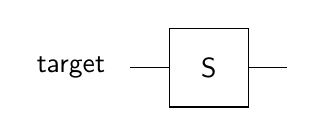
\begin{tikzpicture}[scale=.5] \node[draw=none] at (-3.5, 0) {target}; \draw (-2,0) -- (-1, 0); \draw (1, 0) -- (2, 0); \draw (-1,-1)--(-1,1)--(1,1)--(1,-1)--cycle; \node[draw=none] at (0, 0) {S}; \end{tikzpicture} } \]


\begin{DoxyParams}[1]{Parameters}
\mbox{\tt in,out}  & {\em multi\+Qubit} & object representing the set of all qubits \\
\hline
\mbox{\tt in}  & {\em target\+Qubit} & qubit to operate upon \\
\hline
\end{DoxyParams}

\begin{DoxyExceptions}{Exceptions}
{\em exit\+With\+Error} & if {\ttfamily target\+Qubit} is outside \mbox{[}0, {\ttfamily multi\+Qubit.\+num\+Qubits}) \\
\hline
\end{DoxyExceptions}


Definition at line 1626 of file Qu\+E\+S\+T.\+c.



References phase\+Gate(), and S\+\_\+\+G\+A\+TE.



Referenced by test\+\_\+s\+Gate().


\begin{DoxyCode}
1627 \{
1628     \mbox{\hyperlink{QuEST__env__local_8c_aae7a8a7f1ccbddb7f76b6c52b746bb43}{phaseGate}}(multiQubit, targetQubit, \mbox{\hyperlink{QuEST_8h_a5739021c733cecc49647956b2f7338eaa06e60f80fa80cce271793d6d31bcc21f}{S\_GATE}});
1629 \} 
\end{DoxyCode}
\mbox{\Hypertarget{QuEST_8h_a86e396e06b7d527cac20ba0108872423}\label{QuEST_8h_a86e396e06b7d527cac20ba0108872423}} 
\index{Qu\+E\+S\+T.\+h@{Qu\+E\+S\+T.\+h}!sigmaX@{sigmaX}}
\index{sigmaX@{sigmaX}!Qu\+E\+S\+T.\+h@{Qu\+E\+S\+T.\+h}}
\paragraph{\texorpdfstring{sigma\+X()}{sigmaX()}}
{\footnotesize\ttfamily void sigmaX (\begin{DoxyParamCaption}\item[{\mbox{\hyperlink{structMultiQubit}{Multi\+Qubit}}}]{multi\+Qubit,  }\item[{const int}]{target\+Qubit }\end{DoxyParamCaption})}



Apply the single-\/qubit sigma-\/X (also known as the X, Pauli-\/X, N\+OT or bit-\/flip) gate. 

This is a rotation of $\pi$ around the x-\/axis on the Bloch sphere. I.\+e. \[ \begin{pmatrix} 0 & 1 \\ 1 & 0 \end{pmatrix} \] ~\newline
 \[ \setlength{\fboxrule}{0.01pt} \fbox{ 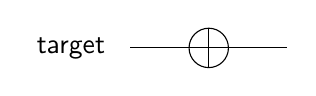
\begin{tikzpicture}[scale=.5] \node[draw=none] at (-3.5, 0) {target}; \draw (-2,0) -- (2, 0); \draw (0, 0) circle (.5); \draw (0, .5) -- (0, -.5); \end{tikzpicture} } \] ~\newline
 
\begin{DoxyParams}[1]{Parameters}
\mbox{\tt in,out}  & {\em multi\+Qubit} & object representing the set of all qubits \\
\hline
\mbox{\tt in}  & {\em target\+Qubit} & qubit to operate on \\
\hline
\end{DoxyParams}

\begin{DoxyExceptions}{Exceptions}
{\em exit\+With\+Error} & if {\ttfamily target\+Qubit} is outside \mbox{[}0, {\ttfamily multi\+Qubit.\+num\+Qubits}). \\
\hline
\end{DoxyExceptions}


Definition at line 151 of file Qu\+E\+S\+T\+\_\+env\+\_\+local.\+c.



References Multi\+Qubit\+::chunk\+Id, chunk\+Is\+Upper(), exchange\+State\+Vectors(), get\+Chunk\+Pair\+Id(), half\+Matrix\+Block\+Fits\+In\+Chunk(), Multi\+Qubit\+::num\+Amps\+Per\+Chunk, Multi\+Qubit\+::num\+Qubits, Multi\+Qubit\+::pair\+State\+Vec, Qu\+E\+S\+T\+Assert(), R\+E\+AL, sigma\+X\+Distributed(), sigma\+X\+Local(), and Multi\+Qubit\+::state\+Vec.



Referenced by main(), and test\+\_\+sigma\+X().


\begin{DoxyCode}
152 \{
153     \mbox{\hyperlink{QuEST__env__local_8c_a3587b9d533e633ccf1abf9ad2ce45d8d}{QuESTAssert}}(targetQubit >= 0 && targetQubit < multiQubit.
      \mbox{\hyperlink{structMultiQubit_ab5b9795bdc6fb5855e1974dcbbaeb36f}{numQubits}}, 1, \_\_func\_\_);
154     \mbox{\hyperlink{QuEST_8c_a74822fd86bb5d81766e6e8dbdcd62df1}{sigmaXLocal}}(multiQubit, targetQubit);
155 \}
\end{DoxyCode}
\mbox{\Hypertarget{QuEST_8h_a1f54d70a42403f7e1c2e2c2007332f61}\label{QuEST_8h_a1f54d70a42403f7e1c2e2c2007332f61}} 
\index{Qu\+E\+S\+T.\+h@{Qu\+E\+S\+T.\+h}!sigmaY@{sigmaY}}
\index{sigmaY@{sigmaY}!Qu\+E\+S\+T.\+h@{Qu\+E\+S\+T.\+h}}
\paragraph{\texorpdfstring{sigma\+Y()}{sigmaY()}}
{\footnotesize\ttfamily void sigmaY (\begin{DoxyParamCaption}\item[{\mbox{\hyperlink{structMultiQubit}{Multi\+Qubit}}}]{multi\+Qubit,  }\item[{const int}]{target\+Qubit }\end{DoxyParamCaption})}



Apply the single-\/qubit sigma-\/Y (also known as the Y or Pauli-\/Y) gate. 

This is a rotation of $\pi$ around the Y-\/axis on the Bloch sphere. I.\+e. \[ \begin{pmatrix} 0 & -i \\ i & 0 \end{pmatrix} \] ~\newline
 \[ \setlength{\fboxrule}{0.01pt} \fbox{ 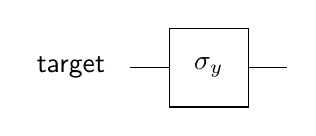
\begin{tikzpicture}[scale=.5] \node[draw=none] at (-3.5, 0) {target}; \draw (-2,0) -- (-1, 0); \draw (1, 0) -- (2, 0); \draw (-1,-1)--(-1,1)--(1,1)--(1,-1)--cycle; \node[draw=none] at (0, 0) {$\sigma_y$}; \end{tikzpicture} } \] ~\newline
 
\begin{DoxyParams}[1]{Parameters}
\mbox{\tt in,out}  & {\em multi\+Qubit} & object representing the set of all qubits \\
\hline
\mbox{\tt in}  & {\em target\+Qubit} & qubit to operate on \\
\hline
\end{DoxyParams}

\begin{DoxyExceptions}{Exceptions}
{\em exit\+With\+Error} & if {\ttfamily target\+Qubit} is outside \mbox{[}0, {\ttfamily multi\+Qubit.\+num\+Qubits}). \\
\hline
\end{DoxyExceptions}
fix -- put duplicate code (sigmaX, sigmaY) in seperate function 

Definition at line 157 of file Qu\+E\+S\+T\+\_\+env\+\_\+local.\+c.



References Multi\+Qubit\+::chunk\+Id, chunk\+Is\+Upper(), exchange\+State\+Vectors(), get\+Chunk\+Pair\+Id(), half\+Matrix\+Block\+Fits\+In\+Chunk(), Multi\+Qubit\+::num\+Amps\+Per\+Chunk, Multi\+Qubit\+::num\+Qubits, Multi\+Qubit\+::pair\+State\+Vec, Qu\+E\+S\+T\+Assert(), R\+E\+AL, sigma\+Y\+Distributed(), sigma\+Y\+Local(), and Multi\+Qubit\+::state\+Vec.



Referenced by test\+\_\+sigma\+Y().


\begin{DoxyCode}
158 \{
159     \mbox{\hyperlink{QuEST__env__local_8c_a3587b9d533e633ccf1abf9ad2ce45d8d}{QuESTAssert}}(targetQubit >= 0 && targetQubit < multiQubit.
      \mbox{\hyperlink{structMultiQubit_ab5b9795bdc6fb5855e1974dcbbaeb36f}{numQubits}}, 1, \_\_func\_\_);
160     \mbox{\hyperlink{QuEST_8c_a81fbfaed65a742a7dfd622e17652245e}{sigmaYLocal}}(multiQubit, targetQubit);
161 \}
\end{DoxyCode}
\mbox{\Hypertarget{QuEST_8h_aebaab86326779de55d335cfea3efde8f}\label{QuEST_8h_aebaab86326779de55d335cfea3efde8f}} 
\index{Qu\+E\+S\+T.\+h@{Qu\+E\+S\+T.\+h}!sigmaZ@{sigmaZ}}
\index{sigmaZ@{sigmaZ}!Qu\+E\+S\+T.\+h@{Qu\+E\+S\+T.\+h}}
\paragraph{\texorpdfstring{sigma\+Z()}{sigmaZ()}}
{\footnotesize\ttfamily void sigmaZ (\begin{DoxyParamCaption}\item[{\mbox{\hyperlink{structMultiQubit}{Multi\+Qubit}}}]{multi\+Qubit,  }\item[{const int}]{target\+Qubit }\end{DoxyParamCaption})}



Apply the single-\/qubit sigma-\/Z (also known as the Z, Pauli-\/Z or phase-\/flip) gate. 

This is a rotation of $\pi$ around the Z-\/axis (a phase shift) on the Bloch sphere. I.\+e. \[ \begin{pmatrix} 1 & 0 \\ 0 & -1 \end{pmatrix} \] ~\newline
 \[ \setlength{\fboxrule}{0.01pt} \fbox{ 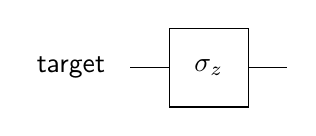
\begin{tikzpicture}[scale=.5] \node[draw=none] at (-3.5, 0) {target}; \draw (-2,0) -- (-1, 0); \draw (1, 0) -- (2, 0); \draw (-1,-1)--(-1,1)--(1,1)--(1,-1)--cycle; \node[draw=none] at (0, 0) {$\sigma_z$}; \end{tikzpicture} } \] ~\newline
 
\begin{DoxyParams}[1]{Parameters}
\mbox{\tt in,out}  & {\em multi\+Qubit} & object representing the set of all qubits \\
\hline
\mbox{\tt in}  & {\em target\+Qubit} & qubit to operate on \\
\hline
\end{DoxyParams}

\begin{DoxyExceptions}{Exceptions}
{\em exit\+With\+Error} & if {\ttfamily target\+Qubit} is outside \mbox{[}0, {\ttfamily multi\+Qubit.\+num\+Qubits}). \\
\hline
\end{DoxyExceptions}


Definition at line 1621 of file Qu\+E\+S\+T.\+c.



References phase\+Gate(), and S\+I\+G\+M\+A\+\_\+Z.



Referenced by test\+\_\+sigma\+Z().


\begin{DoxyCode}
1622 \{
1623     \mbox{\hyperlink{QuEST__env__local_8c_aae7a8a7f1ccbddb7f76b6c52b746bb43}{phaseGate}}(multiQubit, targetQubit, \mbox{\hyperlink{QuEST_8h_a5739021c733cecc49647956b2f7338eaa754922d1e1846a1961ff2bf163483dac}{SIGMA\_Z}});
1624 \}
\end{DoxyCode}
\mbox{\Hypertarget{QuEST_8h_a8d31fe2d1ad4d01e2a1f5f6b8bc15b77}\label{QuEST_8h_a8d31fe2d1ad4d01e2a1f5f6b8bc15b77}} 
\index{Qu\+E\+S\+T.\+h@{Qu\+E\+S\+T.\+h}!sync\+Qu\+E\+S\+T\+Env@{sync\+Qu\+E\+S\+T\+Env}}
\index{sync\+Qu\+E\+S\+T\+Env@{sync\+Qu\+E\+S\+T\+Env}!Qu\+E\+S\+T.\+h@{Qu\+E\+S\+T.\+h}}
\paragraph{\texorpdfstring{sync\+Qu\+E\+S\+T\+Env()}{syncQuESTEnv()}}
{\footnotesize\ttfamily void sync\+Qu\+E\+S\+T\+Env (\begin{DoxyParamCaption}\item[{\mbox{\hyperlink{structQuESTEnv}{Qu\+E\+S\+T\+Env}}}]{env }\end{DoxyParamCaption})}



Guarantees that all code up to the given point has been executed on all nodes (if running in distributed mode) 


\begin{DoxyParams}[1]{Parameters}
\mbox{\tt in}  & {\em env} & object representing the execution environment. A single instance is used for each program \\
\hline
\end{DoxyParams}


Definition at line 31 of file Qu\+E\+S\+T\+\_\+env\+\_\+local.\+c.



Referenced by initialize\+State\+From\+Single\+File(), report\+State\+To\+Screen(), and test\+\_\+controlled\+Not().


\begin{DoxyCode}
31                                \{
32     \textcolor{comment}{// MPI Barrier goes here in MPI version. }
33 \} 
\end{DoxyCode}
\mbox{\Hypertarget{QuEST_8h_ac7e38d768a1bd79019f88cc1e6295092}\label{QuEST_8h_ac7e38d768a1bd79019f88cc1e6295092}} 
\index{Qu\+E\+S\+T.\+h@{Qu\+E\+S\+T.\+h}!sync\+Qu\+E\+S\+T\+Success@{sync\+Qu\+E\+S\+T\+Success}}
\index{sync\+Qu\+E\+S\+T\+Success@{sync\+Qu\+E\+S\+T\+Success}!Qu\+E\+S\+T.\+h@{Qu\+E\+S\+T.\+h}}
\paragraph{\texorpdfstring{sync\+Qu\+E\+S\+T\+Success()}{syncQuESTSuccess()}}
{\footnotesize\ttfamily int sync\+Qu\+E\+S\+T\+Success (\begin{DoxyParamCaption}\item[{int}]{success\+Code }\end{DoxyParamCaption})}



Performs a logical A\+ND on all success\+Codes held by all processes. 

If any one process has a zero success\+Code all processes will return a zero success code.


\begin{DoxyParams}[1]{Parameters}
\mbox{\tt in}  & {\em env} & object representing the execution environment. A single instance is used for each program \\
\hline
\mbox{\tt in}  & {\em success\+Code} & 1 if process task succeeded, 0 if process task failed \\
\hline
\end{DoxyParams}
\begin{DoxyReturn}{Returns}
1 if all processes succeeded, 0 if any one process failed 
\end{DoxyReturn}


Definition at line 35 of file Qu\+E\+S\+T\+\_\+env\+\_\+local.\+c.



Referenced by main().


\begin{DoxyCode}
35                                      \{
36     \textcolor{keywordflow}{return} successCode;
37 \}
\end{DoxyCode}
\mbox{\Hypertarget{QuEST_8h_af764ea63a2e870098f4e1ce08562942e}\label{QuEST_8h_af764ea63a2e870098f4e1ce08562942e}} 
\index{Qu\+E\+S\+T.\+h@{Qu\+E\+S\+T.\+h}!t\+Gate@{t\+Gate}}
\index{t\+Gate@{t\+Gate}!Qu\+E\+S\+T.\+h@{Qu\+E\+S\+T.\+h}}
\paragraph{\texorpdfstring{t\+Gate()}{tGate()}}
{\footnotesize\ttfamily void t\+Gate (\begin{DoxyParamCaption}\item[{\mbox{\hyperlink{structMultiQubit}{Multi\+Qubit}}}]{multi\+Qubit,  }\item[{const int}]{target\+Qubit }\end{DoxyParamCaption})}



Apply the single-\/qubit T gate. 

This is a rotation of $\pi/4$ around the Z-\/axis on the Bloch sphere, or the unitary\+: \[ \begin{pmatrix} 1 & 0 \\ 0 & \exp\left(i \frac{\pi}{4}\right) \end{pmatrix} \]

\[ \setlength{\fboxrule}{0.01pt} \fbox{ 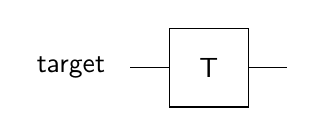
\begin{tikzpicture}[scale=.5] \node[draw=none] at (-3.5, 0) {target}; \draw (-2,0) -- (-1, 0); \draw (1, 0) -- (2, 0); \draw (-1,-1)--(-1,1)--(1,1)--(1,-1)--cycle; \node[draw=none] at (0, 0) {T}; \end{tikzpicture} } \]


\begin{DoxyParams}[1]{Parameters}
\mbox{\tt in,out}  & {\em multi\+Qubit} & object representing the set of all qubits \\
\hline
\mbox{\tt in}  & {\em target\+Qubit} & qubit to operate upon \\
\hline
\end{DoxyParams}

\begin{DoxyExceptions}{Exceptions}
{\em exit\+With\+Error} & if {\ttfamily target\+Qubit} is outside \mbox{[}0, {\ttfamily multi\+Qubit.\+num\+Qubits}) \\
\hline
\end{DoxyExceptions}


Definition at line 1631 of file Qu\+E\+S\+T.\+c.



References phase\+Gate(), and T\+\_\+\+G\+A\+TE.



Referenced by test\+\_\+t\+Gate().


\begin{DoxyCode}
1632 \{
1633     \mbox{\hyperlink{QuEST__env__local_8c_aae7a8a7f1ccbddb7f76b6c52b746bb43}{phaseGate}}(multiQubit, targetQubit, \mbox{\hyperlink{QuEST_8h_a5739021c733cecc49647956b2f7338eaa614d07d597a8e320cc556bc0e652e4ab}{T\_GATE}});
1634 \}
\end{DoxyCode}
\mbox{\Hypertarget{QuEST_8h_a7a0877e33700f6bad48adb51b7b3fb67}\label{QuEST_8h_a7a0877e33700f6bad48adb51b7b3fb67}} 
\index{Qu\+E\+S\+T.\+h@{Qu\+E\+S\+T.\+h}!unitary@{unitary}}
\index{unitary@{unitary}!Qu\+E\+S\+T.\+h@{Qu\+E\+S\+T.\+h}}
\paragraph{\texorpdfstring{unitary()}{unitary()}}
{\footnotesize\ttfamily void unitary (\begin{DoxyParamCaption}\item[{\mbox{\hyperlink{structMultiQubit}{Multi\+Qubit}}}]{multi\+Qubit,  }\item[{const int}]{target\+Qubit,  }\item[{\mbox{\hyperlink{structComplexMatrix2}{Complex\+Matrix2}}}]{u }\end{DoxyParamCaption})}



Apply a general single-\/qubit unitary (including a global phase factor). 

The passed 2x2 Complex\+Matrix must be unitary, otherwise an error is thrown.

\[ \setlength{\fboxrule}{0.01pt} \fbox{ 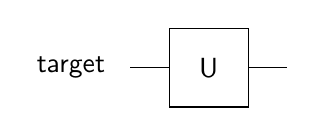
\begin{tikzpicture}[scale=.5] \node[draw=none] at (-3.5, 0) {target}; \draw (-2,0) -- (-1, 0); \draw (1, 0) -- (2, 0); \draw (-1,-1)--(-1,1)--(1,1)--(1,-1)--cycle; \node[draw=none] at (0, 0) {U}; \end{tikzpicture} } \]


\begin{DoxyParams}[1]{Parameters}
\mbox{\tt in,out}  & {\em multi\+Qubit} & object representing the set of all qubits \\
\hline
\mbox{\tt in}  & {\em target\+Qubit} & qubit to operate on \\
\hline
\mbox{\tt in}  & {\em u} & unitary matrix to apply \\
\hline
\end{DoxyParams}

\begin{DoxyExceptions}{Exceptions}
{\em exit\+With\+Error} & if {\ttfamily target\+Qubit} is outside \mbox{[}0, {\ttfamily multi\+Qubit.\+num\+Qubits}), or matrix {\ttfamily u} is not unitary. \\
\hline
\end{DoxyExceptions}


Definition at line 107 of file Qu\+E\+S\+T\+\_\+env\+\_\+local.\+c.



References Multi\+Qubit\+::chunk\+Id, chunk\+Is\+Upper(), exchange\+State\+Vectors(), get\+Chunk\+Pair\+Id(), get\+Rot\+Angle\+From\+Unitary\+Matrix(), half\+Matrix\+Block\+Fits\+In\+Chunk(), Multi\+Qubit\+::num\+Amps\+Per\+Chunk, Multi\+Qubit\+::num\+Qubits, Multi\+Qubit\+::pair\+State\+Vec, Qu\+E\+S\+T\+Assert(), R\+E\+AL, Multi\+Qubit\+::state\+Vec, unitary\+Distributed(), unitary\+Local(), and validate\+Matrix\+Is\+Unitary().



Referenced by main(), and test\+\_\+unitary().


\begin{DoxyCode}
108 \{
109     \mbox{\hyperlink{QuEST__env__local_8c_a3587b9d533e633ccf1abf9ad2ce45d8d}{QuESTAssert}}(targetQubit >= 0 && targetQubit < multiQubit.
      \mbox{\hyperlink{structMultiQubit_ab5b9795bdc6fb5855e1974dcbbaeb36f}{numQubits}}, 1, \_\_func\_\_);
110     \mbox{\hyperlink{QuEST__env__local_8c_a3587b9d533e633ccf1abf9ad2ce45d8d}{QuESTAssert}}(\mbox{\hyperlink{QuEST_8c_ae4fea133d1a8f09ff8da03038100adb2}{validateMatrixIsUnitary}}(u), 5, \_\_func\_\_);
111 
112     \textcolor{comment}{// all values required to update state vector lie in this rank}
113     \mbox{\hyperlink{QuEST_8c_ac134fb45b0a7248c5d15e16eb7139a35}{unitaryLocal}}(multiQubit, targetQubit, u);
114 \}
\end{DoxyCode}

\hypertarget{QuEST__debug_8h}{}\subsection{Qu\+E\+S\+T\+\_\+debug.\+h File Reference}
\label{QuEST__debug_8h}\index{Qu\+E\+S\+T\+\_\+debug.\+h@{Qu\+E\+S\+T\+\_\+debug.\+h}}


Developer functions used for unit testing and debugging.  


{\ttfamily \#include \char`\"{}Qu\+E\+S\+T\+\_\+precision.\+h\char`\"{}}\newline
\subsubsection*{Functions}
\begin{DoxyCompactItemize}
\item 
void \mbox{\hyperlink{QuEST__debug_8h_a7169fd0442cbc3418f3fac4d13363ca2}{init\+State\+Of\+Single\+Qubit}} (\mbox{\hyperlink{structMultiQubit}{Multi\+Qubit}} $\ast$multi\+Qubit, int qubit\+Id, int outcome)
\begin{DoxyCompactList}\small\item\em Initialise the state vector of probability amplitudes such that one qubit is set to \textquotesingle{}outcome\textquotesingle{} and all other qubits are in an equal superposition of zero and one. \end{DoxyCompactList}\item 
void \mbox{\hyperlink{QuEST__debug_8h_a03b3577a891731d505bc4b879fcca9d3}{init\+State\+Debug}} (\mbox{\hyperlink{structMultiQubit}{Multi\+Qubit}} $\ast$multi\+Qubit)
\begin{DoxyCompactList}\small\item\em Initialise the state vector of probability amplitudes to an (unphysical) state with each component of each probability amplitude a unique floating point value. \end{DoxyCompactList}\item 
void \mbox{\hyperlink{QuEST__debug_8h_a433876ee9f3bcc54af346300f571fc3c}{initialize\+State\+From\+Single\+File}} (\mbox{\hyperlink{structMultiQubit}{Multi\+Qubit}} $\ast$multi\+Qubit, char filename\mbox{[}200\mbox{]}, \mbox{\hyperlink{structQuESTEnv}{Qu\+E\+S\+T\+Env}} env)
\item 
int \mbox{\hyperlink{QuEST__debug_8h_a793584932ae384c82e7e42db7d35d18d}{compare\+States}} (\mbox{\hyperlink{structMultiQubit}{Multi\+Qubit}} mq1, \mbox{\hyperlink{structMultiQubit}{Multi\+Qubit}} mq2, \mbox{\hyperlink{QuEST__precision_8h_a4b654506f18b8bfd61ad2a29a7e38c25}{R\+E\+AL}} precision)
\item 
void \mbox{\hyperlink{QuEST__debug_8h_a62da5b58d8ce84e6f4d24be1b872294e}{report\+Node\+List}} (\mbox{\hyperlink{structQuESTEnv}{Qu\+E\+S\+T\+Env}} env)
\begin{DoxyCompactList}\small\item\em Report a list of C\+PU hostnames and the rank that is running on each if running with M\+PI enabled and an error message otherwise. \end{DoxyCompactList}\end{DoxyCompactItemize}


\subsubsection{Detailed Description}
Developer functions used for unit testing and debugging. 

Not part of the public A\+PI. May contain functions that are incomplete or untested. 

\subsubsection{Function Documentation}
\mbox{\Hypertarget{QuEST__debug_8h_a793584932ae384c82e7e42db7d35d18d}\label{QuEST__debug_8h_a793584932ae384c82e7e42db7d35d18d}} 
\index{Qu\+E\+S\+T\+\_\+debug.\+h@{Qu\+E\+S\+T\+\_\+debug.\+h}!compare\+States@{compare\+States}}
\index{compare\+States@{compare\+States}!Qu\+E\+S\+T\+\_\+debug.\+h@{Qu\+E\+S\+T\+\_\+debug.\+h}}
\paragraph{\texorpdfstring{compare\+States()}{compareStates()}}
{\footnotesize\ttfamily int compare\+States (\begin{DoxyParamCaption}\item[{\mbox{\hyperlink{structMultiQubit}{Multi\+Qubit}}}]{mq1,  }\item[{\mbox{\hyperlink{structMultiQubit}{Multi\+Qubit}}}]{mq2,  }\item[{\mbox{\hyperlink{QuEST__precision_8h_a4b654506f18b8bfd61ad2a29a7e38c25}{R\+E\+AL}}}]{precision }\end{DoxyParamCaption})}



Definition at line 372 of file Qu\+E\+S\+T.\+c.



References Complex\+Array\+::imag, Multi\+Qubit\+::num\+Amps, Complex\+Array\+::real, R\+E\+AL, and Multi\+Qubit\+::state\+Vec.


\begin{DoxyCode}
372                                                                  \{
373     \mbox{\hyperlink{QuEST__precision_8h_a4b654506f18b8bfd61ad2a29a7e38c25}{REAL}} diff;
374     \textcolor{keywordtype}{int} chunkSize = mq1.\mbox{\hyperlink{structMultiQubit_ae16f47d8b725c914fb7f66b6498d79db}{numAmps}};
375     \textcolor{keywordflow}{for} (\textcolor{keywordtype}{int} i=0; i<chunkSize; i++)\{
376         diff = fabs(mq1.\mbox{\hyperlink{structMultiQubit_a45483190d6b01ef6b2f98f2bec9ab94f}{stateVec}}.\mbox{\hyperlink{structComplexArray_a4195cac6c784ea1b6271f1c7dba1548a}{real}}[i] - mq2.\mbox{\hyperlink{structMultiQubit_a45483190d6b01ef6b2f98f2bec9ab94f}{stateVec}}.\mbox{\hyperlink{structComplexArray_a4195cac6c784ea1b6271f1c7dba1548a}{real}}[i]);
377         \textcolor{keywordflow}{if} (diff>precision) \textcolor{keywordflow}{return} 0;
378         diff = fabs(mq1.\mbox{\hyperlink{structMultiQubit_a45483190d6b01ef6b2f98f2bec9ab94f}{stateVec}}.\mbox{\hyperlink{structComplexArray_a79dde47c7ae530c79cebfdf57b225968}{imag}}[i] - mq2.\mbox{\hyperlink{structMultiQubit_a45483190d6b01ef6b2f98f2bec9ab94f}{stateVec}}.\mbox{\hyperlink{structComplexArray_a79dde47c7ae530c79cebfdf57b225968}{imag}}[i]);
379         \textcolor{keywordflow}{if} (diff>precision) \textcolor{keywordflow}{return} 0;
380     \}
381     \textcolor{keywordflow}{return} 1;
382 \}
\end{DoxyCode}
\mbox{\Hypertarget{QuEST__debug_8h_a433876ee9f3bcc54af346300f571fc3c}\label{QuEST__debug_8h_a433876ee9f3bcc54af346300f571fc3c}} 
\index{Qu\+E\+S\+T\+\_\+debug.\+h@{Qu\+E\+S\+T\+\_\+debug.\+h}!initialize\+State\+From\+Single\+File@{initialize\+State\+From\+Single\+File}}
\index{initialize\+State\+From\+Single\+File@{initialize\+State\+From\+Single\+File}!Qu\+E\+S\+T\+\_\+debug.\+h@{Qu\+E\+S\+T\+\_\+debug.\+h}}
\paragraph{\texorpdfstring{initialize\+State\+From\+Single\+File()}{initializeStateFromSingleFile()}}
{\footnotesize\ttfamily void initialize\+State\+From\+Single\+File (\begin{DoxyParamCaption}\item[{\mbox{\hyperlink{structMultiQubit}{Multi\+Qubit}} $\ast$}]{multi\+Qubit,  }\item[{char}]{filename\mbox{[}200\mbox{]},  }\item[{\mbox{\hyperlink{structQuESTEnv}{Qu\+E\+S\+T\+Env}}}]{env }\end{DoxyParamCaption})}

fix -- format needs to work for single precision values 

Definition at line 336 of file Qu\+E\+S\+T.\+c.



References Multi\+Qubit\+::chunk\+Id, Complex\+Array\+::imag, Multi\+Qubit\+::num\+Amps, Multi\+Qubit\+::num\+Chunks, Qu\+E\+S\+T\+Assert(), Complex\+Array\+::real, R\+E\+AL, Multi\+Qubit\+::state\+Vec, and sync\+Qu\+E\+S\+T\+Env().


\begin{DoxyCode}
336                                                                                             \{
337     \textcolor{keywordtype}{long} \textcolor{keywordtype}{long} \textcolor{keywordtype}{int} chunkSize, stateVecSize;
338     \textcolor{keywordtype}{long} \textcolor{keywordtype}{long} \textcolor{keywordtype}{int} indexInChunk, totalIndex;
339 
340     chunkSize = multiQubit->\mbox{\hyperlink{structMultiQubit_ae16f47d8b725c914fb7f66b6498d79db}{numAmps}};
341     stateVecSize = chunkSize*multiQubit->\mbox{\hyperlink{structMultiQubit_acd43f2f57991709c9e94f73662c972b2}{numChunks}};
342 
343     \mbox{\hyperlink{QuEST__precision_8h_a4b654506f18b8bfd61ad2a29a7e38c25}{REAL}} *stateVecReal = multiQubit->\mbox{\hyperlink{structMultiQubit_a45483190d6b01ef6b2f98f2bec9ab94f}{stateVec}}.\mbox{\hyperlink{structComplexArray_a4195cac6c784ea1b6271f1c7dba1548a}{real}};
344     \mbox{\hyperlink{QuEST__precision_8h_a4b654506f18b8bfd61ad2a29a7e38c25}{REAL}} *stateVecImag = multiQubit->\mbox{\hyperlink{structMultiQubit_a45483190d6b01ef6b2f98f2bec9ab94f}{stateVec}}.\mbox{\hyperlink{structComplexArray_a79dde47c7ae530c79cebfdf57b225968}{imag}};
345 
346     FILE *fp;
347     \textcolor{keywordtype}{char} line[200];
348 
349     \textcolor{keywordflow}{for} (\textcolor{keywordtype}{int} rank=0; rank<(multiQubit->\mbox{\hyperlink{structMultiQubit_acd43f2f57991709c9e94f73662c972b2}{numChunks}}); rank++)\{
350         \textcolor{keywordflow}{if} (rank==multiQubit->\mbox{\hyperlink{structMultiQubit_ab10c88249fa3825d6227ceec01d37e37}{chunkId}})\{
351             fp = fopen(filename, \textcolor{stringliteral}{"r"});
352             \mbox{\hyperlink{QuEST__env__local_8c_a3587b9d533e633ccf1abf9ad2ce45d8d}{QuESTAssert}}(fp!=NULL, 11, \_\_func\_\_);
353             indexInChunk = 0; totalIndex = 0;
354             \textcolor{keywordflow}{while} (fgets(line, \textcolor{keyword}{sizeof}(\textcolor{keywordtype}{char})*200, fp) != NULL && totalIndex<stateVecSize)\{
355                 \textcolor{keywordflow}{if} (line[0]!=\textcolor{charliteral}{'#'})\{
356                     \textcolor{keywordtype}{int} chunkId = totalIndex/chunkSize;
357                     \textcolor{keywordflow}{if} (chunkId==multiQubit->\mbox{\hyperlink{structMultiQubit_ab10c88249fa3825d6227ceec01d37e37}{chunkId}})\{
359                         sscanf(line, \textcolor{stringliteral}{"%lf, %lf"}, &(stateVecReal[indexInChunk]), 
360                                 &(stateVecImag[indexInChunk]));
361                         indexInChunk += 1;
362                     \}
363                     totalIndex += 1;
364                 \}
365             \}   
366             fclose(fp);
367         \}
368         \mbox{\hyperlink{QuEST_8h_a8d31fe2d1ad4d01e2a1f5f6b8bc15b77}{syncQuESTEnv}}(env);
369     \}
370 \}
\end{DoxyCode}
\mbox{\Hypertarget{QuEST__debug_8h_a03b3577a891731d505bc4b879fcca9d3}\label{QuEST__debug_8h_a03b3577a891731d505bc4b879fcca9d3}} 
\index{Qu\+E\+S\+T\+\_\+debug.\+h@{Qu\+E\+S\+T\+\_\+debug.\+h}!init\+State\+Debug@{init\+State\+Debug}}
\index{init\+State\+Debug@{init\+State\+Debug}!Qu\+E\+S\+T\+\_\+debug.\+h@{Qu\+E\+S\+T\+\_\+debug.\+h}}
\paragraph{\texorpdfstring{init\+State\+Debug()}{initStateDebug()}}
{\footnotesize\ttfamily void init\+State\+Debug (\begin{DoxyParamCaption}\item[{\mbox{\hyperlink{structMultiQubit}{Multi\+Qubit}} $\ast$}]{multi\+Qubit }\end{DoxyParamCaption})}



Initialise the state vector of probability amplitudes to an (unphysical) state with each component of each probability amplitude a unique floating point value. 

For debugging processes 
\begin{DoxyParams}[1]{Parameters}
\mbox{\tt in,out}  & {\em multi\+Qubit} & object representing the set of qubits to be initialised \\
\hline
\end{DoxyParams}


Definition at line 304 of file Qu\+E\+S\+T.\+c.



References Multi\+Qubit\+::chunk\+Id, Complex\+Array\+::imag, Multi\+Qubit\+::num\+Amps, Complex\+Array\+::real, R\+E\+AL, and Multi\+Qubit\+::state\+Vec.


\begin{DoxyCode}
305 \{
306     \textcolor{keywordtype}{long} \textcolor{keywordtype}{long} \textcolor{keywordtype}{int} chunkSize;
307     \textcolor{keywordtype}{long} \textcolor{keywordtype}{long} \textcolor{keywordtype}{int} index;
308 
309     \textcolor{comment}{// dimension of the state vector}
310     chunkSize = multiQubit->\mbox{\hyperlink{structMultiQubit_ae16f47d8b725c914fb7f66b6498d79db}{numAmps}};
311 
312     \textcolor{comment}{// Can't use multiQubit->stateVec as a private OMP var}
313     \mbox{\hyperlink{QuEST__precision_8h_a4b654506f18b8bfd61ad2a29a7e38c25}{REAL}} *stateVecReal = multiQubit->\mbox{\hyperlink{structMultiQubit_a45483190d6b01ef6b2f98f2bec9ab94f}{stateVec}}.\mbox{\hyperlink{structComplexArray_a4195cac6c784ea1b6271f1c7dba1548a}{real}};
314     \mbox{\hyperlink{QuEST__precision_8h_a4b654506f18b8bfd61ad2a29a7e38c25}{REAL}} *stateVecImag = multiQubit->\mbox{\hyperlink{structMultiQubit_a45483190d6b01ef6b2f98f2bec9ab94f}{stateVec}}.\mbox{\hyperlink{structComplexArray_a79dde47c7ae530c79cebfdf57b225968}{imag}};
315 
316     \mbox{\hyperlink{QuEST__precision_8h_a4b654506f18b8bfd61ad2a29a7e38c25}{REAL}} chunkOffset = (2.0*chunkSize*multiQubit->\mbox{\hyperlink{structMultiQubit_ab10c88249fa3825d6227ceec01d37e37}{chunkId}})/10.0;
317 
318     \textcolor{comment}{// initialise the state to |0000..0000>}
319 \textcolor{preprocessor}{# ifdef \_OPENMP}
320 \textcolor{preprocessor}{# pragma omp parallel \(\backslash\)}
321 \textcolor{preprocessor}{    default  (none) \(\backslash\)}
322 \textcolor{preprocessor}{    shared   (chunkSize, stateVecReal, stateVecImag, chunkOffset) \(\backslash\)}
323 \textcolor{preprocessor}{    private  (index) }
324 \textcolor{preprocessor}{# endif}
325     \{
326 \textcolor{preprocessor}{# ifdef \_OPENMP}
327 \textcolor{preprocessor}{# pragma omp for schedule (static)}
328 \textcolor{preprocessor}{# endif}
329         \textcolor{keywordflow}{for} (index=0; index<chunkSize; index++) \{
330             stateVecReal[index] = chunkOffset + (index*2.0)/10.0;
331             stateVecImag[index] = chunkOffset + (index*2.0+1.0)/10.0;
332         \}
333     \}
334 \}
\end{DoxyCode}
\mbox{\Hypertarget{QuEST__debug_8h_a7169fd0442cbc3418f3fac4d13363ca2}\label{QuEST__debug_8h_a7169fd0442cbc3418f3fac4d13363ca2}} 
\index{Qu\+E\+S\+T\+\_\+debug.\+h@{Qu\+E\+S\+T\+\_\+debug.\+h}!init\+State\+Of\+Single\+Qubit@{init\+State\+Of\+Single\+Qubit}}
\index{init\+State\+Of\+Single\+Qubit@{init\+State\+Of\+Single\+Qubit}!Qu\+E\+S\+T\+\_\+debug.\+h@{Qu\+E\+S\+T\+\_\+debug.\+h}}
\paragraph{\texorpdfstring{init\+State\+Of\+Single\+Qubit()}{initStateOfSingleQubit()}}
{\footnotesize\ttfamily void init\+State\+Of\+Single\+Qubit (\begin{DoxyParamCaption}\item[{\mbox{\hyperlink{structMultiQubit}{Multi\+Qubit}} $\ast$}]{multi\+Qubit,  }\item[{int}]{qubit\+Id,  }\item[{int}]{outcome }\end{DoxyParamCaption})}



Initialise the state vector of probability amplitudes such that one qubit is set to \textquotesingle{}outcome\textquotesingle{} and all other qubits are in an equal superposition of zero and one. 


\begin{DoxyParams}[1]{Parameters}
\mbox{\tt in,out}  & {\em multi\+Qubit} & object representing the set of qubits to be initialised \\
\hline
\mbox{\tt in}  & {\em qubit\+Id} & id of qubit to set to state \textquotesingle{}outcome\textquotesingle{} \\
\hline
\mbox{\tt in}  & {\em value} & of qubit \textquotesingle{}qubit\+Id\textquotesingle{} \\
\hline
\end{DoxyParams}


Definition at line 258 of file Qu\+E\+S\+T.\+c.



References Multi\+Qubit\+::chunk\+Id, extract\+Bit(), Complex\+Array\+::imag, Multi\+Qubit\+::num\+Amps, Multi\+Qubit\+::num\+Chunks, Complex\+Array\+::real, R\+E\+AL, and Multi\+Qubit\+::state\+Vec.


\begin{DoxyCode}
259 \{
260     \textcolor{keywordtype}{long} \textcolor{keywordtype}{long} \textcolor{keywordtype}{int} chunkSize, stateVecSize;
261     \textcolor{keywordtype}{long} \textcolor{keywordtype}{long} \textcolor{keywordtype}{int} index;
262     \textcolor{keywordtype}{int} bit;
263     \textcolor{keyword}{const} \textcolor{keywordtype}{long} \textcolor{keywordtype}{long} \textcolor{keywordtype}{int} chunkId=multiQubit->\mbox{\hyperlink{structMultiQubit_ab10c88249fa3825d6227ceec01d37e37}{chunkId}};
264 
265     \textcolor{comment}{// dimension of the state vector}
266     chunkSize = multiQubit->\mbox{\hyperlink{structMultiQubit_ae16f47d8b725c914fb7f66b6498d79db}{numAmps}};
267     stateVecSize = chunkSize*multiQubit->\mbox{\hyperlink{structMultiQubit_acd43f2f57991709c9e94f73662c972b2}{numChunks}};
268     \mbox{\hyperlink{QuEST__precision_8h_a4b654506f18b8bfd61ad2a29a7e38c25}{REAL}} normFactor = 1.0/sqrt((\mbox{\hyperlink{QuEST__precision_8h_a4b654506f18b8bfd61ad2a29a7e38c25}{REAL}})stateVecSize/2.0);
269 
270     \textcolor{comment}{// Can't use multiQubit->stateVec as a private OMP var}
271     \mbox{\hyperlink{QuEST__precision_8h_a4b654506f18b8bfd61ad2a29a7e38c25}{REAL}} *stateVecReal = multiQubit->\mbox{\hyperlink{structMultiQubit_a45483190d6b01ef6b2f98f2bec9ab94f}{stateVec}}.\mbox{\hyperlink{structComplexArray_a4195cac6c784ea1b6271f1c7dba1548a}{real}};
272     \mbox{\hyperlink{QuEST__precision_8h_a4b654506f18b8bfd61ad2a29a7e38c25}{REAL}} *stateVecImag = multiQubit->\mbox{\hyperlink{structMultiQubit_a45483190d6b01ef6b2f98f2bec9ab94f}{stateVec}}.\mbox{\hyperlink{structComplexArray_a79dde47c7ae530c79cebfdf57b225968}{imag}};
273 
274     \textcolor{comment}{// initialise the state to |0000..0000>}
275 \textcolor{preprocessor}{# ifdef \_OPENMP}
276 \textcolor{preprocessor}{# pragma omp parallel \(\backslash\)}
277 \textcolor{preprocessor}{    default  (none) \(\backslash\)}
278 \textcolor{preprocessor}{    shared   (chunkSize, stateVecReal, stateVecImag, normFactor, qubitId, outcome) \(\backslash\)}
279 \textcolor{preprocessor}{    private  (index, bit) }
280 \textcolor{preprocessor}{# endif}
281     \{
282 \textcolor{preprocessor}{# ifdef \_OPENMP}
283 \textcolor{preprocessor}{# pragma omp for schedule (static)}
284 \textcolor{preprocessor}{# endif}
285         \textcolor{keywordflow}{for} (index=0; index<chunkSize; index++) \{
286             bit = \mbox{\hyperlink{QuEST_8c_a100463f6ec212c76a5fad99579000505}{extractBit}}(qubitId, index+chunkId*chunkSize);
287             \textcolor{keywordflow}{if} (bit==outcome) \{
288                 stateVecReal[index] = normFactor;
289                 stateVecImag[index] = 0.0;
290             \} \textcolor{keywordflow}{else} \{
291                 stateVecReal[index] = 0.0;
292                 stateVecImag[index] = 0.0;
293             \}
294         \}
295     \}
296 \}
\end{DoxyCode}
\mbox{\Hypertarget{QuEST__debug_8h_a62da5b58d8ce84e6f4d24be1b872294e}\label{QuEST__debug_8h_a62da5b58d8ce84e6f4d24be1b872294e}} 
\index{Qu\+E\+S\+T\+\_\+debug.\+h@{Qu\+E\+S\+T\+\_\+debug.\+h}!report\+Node\+List@{report\+Node\+List}}
\index{report\+Node\+List@{report\+Node\+List}!Qu\+E\+S\+T\+\_\+debug.\+h@{Qu\+E\+S\+T\+\_\+debug.\+h}}
\paragraph{\texorpdfstring{report\+Node\+List()}{reportNodeList()}}
{\footnotesize\ttfamily void report\+Node\+List (\begin{DoxyParamCaption}\item[{\mbox{\hyperlink{structQuESTEnv}{Qu\+E\+S\+T\+Env}}}]{env }\end{DoxyParamCaption})}



Report a list of C\+PU hostnames and the rank that is running on each if running with M\+PI enabled and an error message otherwise. 

For debugging purposes. 
\begin{DoxyParams}[1]{Parameters}
\mbox{\tt in}  & {\em env} & object representing the execution environment. A single instance is used for each program \\
\hline
\end{DoxyParams}


Definition at line 53 of file Qu\+E\+S\+T\+\_\+env\+\_\+local.\+c.



References Qu\+E\+S\+T\+Env\+::rank.


\begin{DoxyCode}
53                                  \{
54     printf(\textcolor{stringliteral}{"Hostname unknown: running locally\(\backslash\)n"});
55 \}
\end{DoxyCode}

\hypertarget{QuEST__precision_8h}{}\subsection{Qu\+E\+S\+T\+\_\+precision.\+h File Reference}
\label{QuEST__precision_8h}\index{Qu\+E\+S\+T\+\_\+precision.\+h@{Qu\+E\+S\+T\+\_\+precision.\+h}}
\subsubsection*{Macros}
\begin{DoxyCompactItemize}
\item 
\#define \mbox{\hyperlink{QuEST__precision_8h_a2bda1a81ce3474772a8a1f165e54516e}{P\+R\+EC}}~2
\item 
\#define \mbox{\hyperlink{QuEST__precision_8h_a4b654506f18b8bfd61ad2a29a7e38c25}{R\+E\+AL}}~double
\item 
\#define \mbox{\hyperlink{QuEST__precision_8h_a750ad290949ef7dc4afdfbd8231a5057}{M\+P\+I\+\_\+\+Qu\+E\+S\+T\+\_\+\+R\+E\+AL}}~M\+P\+I\+\_\+\+D\+O\+U\+B\+LE
\item 
\#define \mbox{\hyperlink{QuEST__precision_8h_ad751ac7ddc8ec19f23fb33083c0da8da}{R\+E\+A\+L\+\_\+\+S\+T\+R\+I\+N\+G\+\_\+\+F\+O\+R\+M\+AT}}~\char`\"{}\%.\+14f\char`\"{}
\item 
\#define \mbox{\hyperlink{QuEST__precision_8h_aebb5e6716e06431296af4d1a71744dec}{R\+E\+A\+L\+\_\+\+E\+PS}}~1e-\/13
\end{DoxyCompactItemize}


\subsubsection{Macro Definition Documentation}
\mbox{\Hypertarget{QuEST__precision_8h_a750ad290949ef7dc4afdfbd8231a5057}\label{QuEST__precision_8h_a750ad290949ef7dc4afdfbd8231a5057}} 
\index{Qu\+E\+S\+T\+\_\+precision.\+h@{Qu\+E\+S\+T\+\_\+precision.\+h}!M\+P\+I\+\_\+\+Qu\+E\+S\+T\+\_\+\+R\+E\+AL@{M\+P\+I\+\_\+\+Qu\+E\+S\+T\+\_\+\+R\+E\+AL}}
\index{M\+P\+I\+\_\+\+Qu\+E\+S\+T\+\_\+\+R\+E\+AL@{M\+P\+I\+\_\+\+Qu\+E\+S\+T\+\_\+\+R\+E\+AL}!Qu\+E\+S\+T\+\_\+precision.\+h@{Qu\+E\+S\+T\+\_\+precision.\+h}}
\paragraph{\texorpdfstring{M\+P\+I\+\_\+\+Qu\+E\+S\+T\+\_\+\+R\+E\+AL}{MPI\_QuEST\_REAL}}
{\footnotesize\ttfamily \#define M\+P\+I\+\_\+\+Qu\+E\+S\+T\+\_\+\+R\+E\+AL~M\+P\+I\+\_\+\+D\+O\+U\+B\+LE}



Definition at line 26 of file Qu\+E\+S\+T\+\_\+precision.\+h.



Referenced by calc\+Total\+Probability(), exchange\+State\+Vectors(), find\+Probability\+Of\+Outcome(), get\+Imag\+Amp\+El(), and get\+Real\+Amp\+El().

\mbox{\Hypertarget{QuEST__precision_8h_a2bda1a81ce3474772a8a1f165e54516e}\label{QuEST__precision_8h_a2bda1a81ce3474772a8a1f165e54516e}} 
\index{Qu\+E\+S\+T\+\_\+precision.\+h@{Qu\+E\+S\+T\+\_\+precision.\+h}!P\+R\+EC@{P\+R\+EC}}
\index{P\+R\+EC@{P\+R\+EC}!Qu\+E\+S\+T\+\_\+precision.\+h@{Qu\+E\+S\+T\+\_\+precision.\+h}}
\paragraph{\texorpdfstring{P\+R\+EC}{PREC}}
{\footnotesize\ttfamily \#define P\+R\+EC~2}



Definition at line 8 of file Qu\+E\+S\+T\+\_\+precision.\+h.

\mbox{\Hypertarget{QuEST__precision_8h_a4b654506f18b8bfd61ad2a29a7e38c25}\label{QuEST__precision_8h_a4b654506f18b8bfd61ad2a29a7e38c25}} 
\index{Qu\+E\+S\+T\+\_\+precision.\+h@{Qu\+E\+S\+T\+\_\+precision.\+h}!R\+E\+AL@{R\+E\+AL}}
\index{R\+E\+AL@{R\+E\+AL}!Qu\+E\+S\+T\+\_\+precision.\+h@{Qu\+E\+S\+T\+\_\+precision.\+h}}
\paragraph{\texorpdfstring{R\+E\+AL}{REAL}}
{\footnotesize\ttfamily \#define R\+E\+AL~double}



Definition at line 25 of file Qu\+E\+S\+T\+\_\+precision.\+h.



Referenced by calc\+Total\+Probability(), collapse\+To\+Outcome(), collapse\+To\+Outcome\+Distributed\+Renorm(), collapse\+To\+Outcome\+Distributed\+Set\+Zero(), collapse\+To\+Outcome\+Local(), compact\+Unitary\+Distributed(), compact\+Unitary\+Local(), compare\+States(), controlled\+Compact\+Unitary\+Distributed(), controlled\+Compact\+Unitary\+Local(), controlled\+Not\+Distributed(), controlled\+Not\+Local(), controlled\+Phase\+Gate(), controlled\+Unitary\+Distributed(), controlled\+Unitary\+Local(), exchange\+State\+Vectors(), find\+Probability\+Of\+Outcome(), find\+Probability\+Of\+Zero\+Distributed(), find\+Probability\+Of\+Zero\+Local(), get\+Imag\+Amp\+El(), get\+Prob\+El(), get\+Real\+Amp\+El(), hadamard\+Distributed(), hadamard\+Local(), init\+Classical\+State(), initialize\+State\+From\+Single\+File(), init\+State\+Debug(), init\+State\+Of\+Single\+Qubit(), init\+State\+Plus(), init\+State\+Zero(), main(), measure(), measure\+With\+Stats(), multi\+Controlled\+Phase\+Gate(), multi\+Controlled\+Unitary\+Distributed(), multi\+Controlled\+Unitary\+Local(), phase\+Gate\+Distributed(), phase\+Gate\+Local(), report\+Qu\+E\+S\+T\+Env(), sigma\+X\+Distributed(), sigma\+X\+Local(), sigma\+Y\+Distributed(), sigma\+Y\+Local(), unitary\+Distributed(), and unitary\+Local().

\mbox{\Hypertarget{QuEST__precision_8h_aebb5e6716e06431296af4d1a71744dec}\label{QuEST__precision_8h_aebb5e6716e06431296af4d1a71744dec}} 
\index{Qu\+E\+S\+T\+\_\+precision.\+h@{Qu\+E\+S\+T\+\_\+precision.\+h}!R\+E\+A\+L\+\_\+\+E\+PS@{R\+E\+A\+L\+\_\+\+E\+PS}}
\index{R\+E\+A\+L\+\_\+\+E\+PS@{R\+E\+A\+L\+\_\+\+E\+PS}!Qu\+E\+S\+T\+\_\+precision.\+h@{Qu\+E\+S\+T\+\_\+precision.\+h}}
\paragraph{\texorpdfstring{R\+E\+A\+L\+\_\+\+E\+PS}{REAL\_EPS}}
{\footnotesize\ttfamily \#define R\+E\+A\+L\+\_\+\+E\+PS~1e-\/13}



Definition at line 28 of file Qu\+E\+S\+T\+\_\+precision.\+h.



Referenced by collapse\+To\+Outcome(), measure\+With\+Stats(), validate\+Alpha\+Beta(), validate\+Matrix\+Is\+Unitary(), and validate\+Unit\+Vector().

\mbox{\Hypertarget{QuEST__precision_8h_ad751ac7ddc8ec19f23fb33083c0da8da}\label{QuEST__precision_8h_ad751ac7ddc8ec19f23fb33083c0da8da}} 
\index{Qu\+E\+S\+T\+\_\+precision.\+h@{Qu\+E\+S\+T\+\_\+precision.\+h}!R\+E\+A\+L\+\_\+\+S\+T\+R\+I\+N\+G\+\_\+\+F\+O\+R\+M\+AT@{R\+E\+A\+L\+\_\+\+S\+T\+R\+I\+N\+G\+\_\+\+F\+O\+R\+M\+AT}}
\index{R\+E\+A\+L\+\_\+\+S\+T\+R\+I\+N\+G\+\_\+\+F\+O\+R\+M\+AT@{R\+E\+A\+L\+\_\+\+S\+T\+R\+I\+N\+G\+\_\+\+F\+O\+R\+M\+AT}!Qu\+E\+S\+T\+\_\+precision.\+h@{Qu\+E\+S\+T\+\_\+precision.\+h}}
\paragraph{\texorpdfstring{R\+E\+A\+L\+\_\+\+S\+T\+R\+I\+N\+G\+\_\+\+F\+O\+R\+M\+AT}{REAL\_STRING\_FORMAT}}
{\footnotesize\ttfamily \#define R\+E\+A\+L\+\_\+\+S\+T\+R\+I\+N\+G\+\_\+\+F\+O\+R\+M\+AT~\char`\"{}\%.\+14f\char`\"{}}



Definition at line 27 of file Qu\+E\+S\+T\+\_\+precision.\+h.



Referenced by report\+State(), and report\+State\+To\+Screen().


\hypertarget{README_8md}{
\subsection{README.md File Reference}
\label{README_8md}\index{README.md@{README.md}}
}
\subsubsection*{Functions}
\begin{DoxyCompactItemize}
\item 
\hyperlink{README_8md_a919bff7d5f7b67fde28e771903fff6f1}{controlledNot} (qubits, 0, 1)
\item 
\hyperlink{README_8md_a6f495fc15ce3f43b4c8adbf43cb881ea}{rotateY} (qubits, 0,.1)
\item 
\hyperlink{README_8md_ac4cb8c0825f6c6a74b839bbd4ae22ea4}{rotateAroundAxis} (qubits, 0, 3.14/2, \hyperlink{README_8md_a22eb3b09da74633038e36bd8dfef55c0}{v})
\item 
\hyperlink{README_8md_a22b5a2d7f987c5e030a1d683d9483f49}{unitary} (qubits, 0, \hyperlink{README_8md_a5d1c311241dc8d8ffa4badf059977dc5}{u})
\item 
\hyperlink{README_8md_a25572bc3f038713ed311fea2b40de0e9}{multiControlledUnitary} (qureg, \hyperlink{README_8md_a636f16bb55903420974dfd184205e591}{controls}, 5, 0, \hyperlink{README_8md_a5d1c311241dc8d8ffa4badf059977dc5}{u})
\end{DoxyCompactItemize}
\subsubsection*{Variables}
\begin{DoxyCompactItemize}
\item 
\hyperlink{README_8md_a2d0f5bba181ef1543dc90d4f1ce64c5e}{QuEST} is currently in prerelease and may be unstable Latest \hyperlink{README_8md_a94df19ae37ab2d673ea00c5d31754e61}{version}
\item 
though is flexible C \hyperlink{structVector}{Vector} \hyperlink{README_8md_a22eb3b09da74633038e36bd8dfef55c0}{v}
\item 
\hyperlink{README_8md_a22eb3b09da74633038e36bd8dfef55c0}{v} \hyperlink{README_8md_a6a52a27535805eddc782c67f42c20c69}{x} = 1
\item 
\hyperlink{README_8md_a22eb3b09da74633038e36bd8dfef55c0}{v} \hyperlink{README_8md_a003dc5701d53a819228f5417a8089139}{y} = 0
\item 
\hyperlink{README_8md_a22eb3b09da74633038e36bd8dfef55c0}{v} \hyperlink{README_8md_a0f9f545825a114923b98de8cc33a5f6a}{z} = 0
\item 
and powerful C \hyperlink{structComplexMatrix2}{ComplexMatrix2} \hyperlink{README_8md_a5d1c311241dc8d8ffa4badf059977dc5}{u}
\item 
\hyperlink{README_8md_a5d1c311241dc8d8ffa4badf059977dc5}{u} \hyperlink{README_8md_a28c529de4915322d2a51f2c1a424c672}{r0c0} = (\hyperlink{structComplex}{Complex}) \{.real=.5, .imag= .5\}
\item 
\hyperlink{README_8md_a5d1c311241dc8d8ffa4badf059977dc5}{u} \hyperlink{README_8md_a444db2ee26ed224e9370770814cb4b50}{r0c1} = (\hyperlink{structComplex}{Complex}) \{.real=.5, .imag=-\/.5\}
\item 
\hyperlink{README_8md_a5d1c311241dc8d8ffa4badf059977dc5}{u} \hyperlink{README_8md_a698aa54017453fbfbf429e0e46821ef8}{r1c0} = (\hyperlink{structComplex}{Complex}) \{.real=.5, .imag=-\/.5\}
\item 
\hyperlink{README_8md_a5d1c311241dc8d8ffa4badf059977dc5}{u} \hyperlink{README_8md_aae8b0c0e5cc303f7560cb29107cd0787}{r1c1} = (\hyperlink{structComplex}{Complex}) \{.real=.5, .imag= .5\}
\item 
int\mbox{[}$\,$\mbox{]} \hyperlink{README_8md_a636f16bb55903420974dfd184205e591}{controls} = \{1, 2, 3, 4, 5\}
\item 
\hyperlink{README_8md_a2d0f5bba181ef1543dc90d4f1ce64c5e}{QuEST} is contained entirely in the c and h files in the \hyperlink{README_8md_a2d0f5bba181ef1543dc90d4f1ce64c5e}{QuEST} folder To use \hyperlink{README_8md_a2d0f5bba181ef1543dc90d4f1ce64c5e}{QuEST}
\end{DoxyCompactItemize}


\subsubsection{Function Documentation}
\hypertarget{README_8md_a919bff7d5f7b67fde28e771903fff6f1}{
\index{README.md@{README.md}!controlledNot@{controlledNot}}
\index{controlledNot@{controlledNot}!README.md@{README.md}}
\paragraph[{controlledNot}]{\setlength{\rightskip}{0pt plus 5cm}controlledNot (qubits, \/  0, \/  1)}\hfill}
\label{README_8md_a919bff7d5f7b67fde28e771903fff6f1}
\hypertarget{README_8md_a25572bc3f038713ed311fea2b40de0e9}{
\index{README.md@{README.md}!multiControlledUnitary@{multiControlledUnitary}}
\index{multiControlledUnitary@{multiControlledUnitary}!README.md@{README.md}}
\paragraph[{multiControlledUnitary}]{\setlength{\rightskip}{0pt plus 5cm}multiControlledUnitary (qureg, \/  {\bf controls}, \/  5, \/  0, \/  {\bf u})}\hfill}
\label{README_8md_a25572bc3f038713ed311fea2b40de0e9}
\hypertarget{README_8md_ac4cb8c0825f6c6a74b839bbd4ae22ea4}{
\index{README.md@{README.md}!rotateAroundAxis@{rotateAroundAxis}}
\index{rotateAroundAxis@{rotateAroundAxis}!README.md@{README.md}}
\paragraph[{rotateAroundAxis}]{\setlength{\rightskip}{0pt plus 5cm}rotateAroundAxis (qubits, \/  0, \/  3.14/ {\em 2}, \/  {\bf v})}\hfill}
\label{README_8md_ac4cb8c0825f6c6a74b839bbd4ae22ea4}
\hypertarget{README_8md_a6f495fc15ce3f43b4c8adbf43cb881ea}{
\index{README.md@{README.md}!rotateY@{rotateY}}
\index{rotateY@{rotateY}!README.md@{README.md}}
\paragraph[{rotateY}]{\setlength{\rightskip}{0pt plus 5cm}rotateY (qubits, \/  0, \/  . {\em 1})}\hfill}
\label{README_8md_a6f495fc15ce3f43b4c8adbf43cb881ea}
\hypertarget{README_8md_a22b5a2d7f987c5e030a1d683d9483f49}{
\index{README.md@{README.md}!unitary@{unitary}}
\index{unitary@{unitary}!README.md@{README.md}}
\paragraph[{unitary}]{\setlength{\rightskip}{0pt plus 5cm}unitary (qubits, \/  0, \/  {\bf u})}\hfill}
\label{README_8md_a22b5a2d7f987c5e030a1d683d9483f49}


\subsubsection{Variable Documentation}
\hypertarget{README_8md_a636f16bb55903420974dfd184205e591}{
\index{README.md@{README.md}!controls@{controls}}
\index{controls@{controls}!README.md@{README.md}}
\paragraph[{controls}]{\setlength{\rightskip}{0pt plus 5cm}int \mbox{[}$\,$\mbox{]} {\bf controls} = \{1, 2, 3, 4, 5\}}\hfill}
\label{README_8md_a636f16bb55903420974dfd184205e591}


Definition at line 59 of file README.md.\hypertarget{README_8md_a2d0f5bba181ef1543dc90d4f1ce64c5e}{
\index{README.md@{README.md}!QuEST@{QuEST}}
\index{QuEST@{QuEST}!README.md@{README.md}}
\paragraph[{QuEST}]{\setlength{\rightskip}{0pt plus 5cm}{\bf QuEST} is contained entirely in the c and h files in the {\bf QuEST} folder To use copy these files to your computer and include {\bf QuEST} h in your C code We include make files for compiling {\bf QuEST}}\hfill}
\label{README_8md_a2d0f5bba181ef1543dc90d4f1ce64c5e}


Definition at line 65 of file README.md.\hypertarget{README_8md_a28c529de4915322d2a51f2c1a424c672}{
\index{README.md@{README.md}!r0c0@{r0c0}}
\index{r0c0@{r0c0}!README.md@{README.md}}
\paragraph[{r0c0}]{\setlength{\rightskip}{0pt plus 5cm}{\bf u} {\bf r0c0} = ({\bf Complex}) \{.real=.5, .imag= .5\}}\hfill}
\label{README_8md_a28c529de4915322d2a51f2c1a424c672}


Definition at line 53 of file README.md.\hypertarget{README_8md_a444db2ee26ed224e9370770814cb4b50}{
\index{README.md@{README.md}!r0c1@{r0c1}}
\index{r0c1@{r0c1}!README.md@{README.md}}
\paragraph[{r0c1}]{\setlength{\rightskip}{0pt plus 5cm}{\bf u} {\bf r0c1} = ({\bf Complex}) \{.real=.5, .imag=-\/.5\}}\hfill}
\label{README_8md_a444db2ee26ed224e9370770814cb4b50}


Definition at line 54 of file README.md.\hypertarget{README_8md_a698aa54017453fbfbf429e0e46821ef8}{
\index{README.md@{README.md}!r1c0@{r1c0}}
\index{r1c0@{r1c0}!README.md@{README.md}}
\paragraph[{r1c0}]{\setlength{\rightskip}{0pt plus 5cm}{\bf u} {\bf r1c0} = ({\bf Complex}) \{.real=.5, .imag=-\/.5\}}\hfill}
\label{README_8md_a698aa54017453fbfbf429e0e46821ef8}


Definition at line 55 of file README.md.\hypertarget{README_8md_aae8b0c0e5cc303f7560cb29107cd0787}{
\index{README.md@{README.md}!r1c1@{r1c1}}
\index{r1c1@{r1c1}!README.md@{README.md}}
\paragraph[{r1c1}]{\setlength{\rightskip}{0pt plus 5cm}{\bf u} {\bf r1c1} = ({\bf Complex}) \{.real=.5, .imag= .5\}}\hfill}
\label{README_8md_aae8b0c0e5cc303f7560cb29107cd0787}


Definition at line 56 of file README.md.\hypertarget{README_8md_a5d1c311241dc8d8ffa4badf059977dc5}{
\index{README.md@{README.md}!u@{u}}
\index{u@{u}!README.md@{README.md}}
\paragraph[{u}]{\setlength{\rightskip}{0pt plus 5cm}and powerful C {\bf ComplexMatrix2} {\bf u}}\hfill}
\label{README_8md_a5d1c311241dc8d8ffa4badf059977dc5}


Definition at line 52 of file README.md.

Referenced by main(), test\_\-controlledUnitary(), test\_\-multiControlledUnitary(), and test\_\-unitary().\hypertarget{README_8md_a22eb3b09da74633038e36bd8dfef55c0}{
\index{README.md@{README.md}!v@{v}}
\index{v@{v}!README.md@{README.md}}
\paragraph[{v}]{\setlength{\rightskip}{0pt plus 5cm}though is flexible C {\bf Vector} {\bf v}}\hfill}
\label{README_8md_a22eb3b09da74633038e36bd8dfef55c0}


Definition at line 46 of file README.md.

Referenced by main().\hypertarget{README_8md_a94df19ae37ab2d673ea00c5d31754e61}{
\index{README.md@{README.md}!version@{version}}
\index{version@{version}!README.md@{README.md}}
\paragraph[{version}]{\setlength{\rightskip}{0pt plus 5cm}{\bf QuEST} is currently in prerelease and may be unstable Latest {\bf version}}\hfill}
\label{README_8md_a94df19ae37ab2d673ea00c5d31754e61}


Definition at line 15 of file README.md.\hypertarget{README_8md_a6a52a27535805eddc782c67f42c20c69}{
\index{README.md@{README.md}!x@{x}}
\index{x@{x}!README.md@{README.md}}
\paragraph[{x}]{\setlength{\rightskip}{0pt plus 5cm}{\bf v} {\bf x} = 1}\hfill}
\label{README_8md_a6a52a27535805eddc782c67f42c20c69}


Definition at line 47 of file README.md.\hypertarget{README_8md_a003dc5701d53a819228f5417a8089139}{
\index{README.md@{README.md}!y@{y}}
\index{y@{y}!README.md@{README.md}}
\paragraph[{y}]{\setlength{\rightskip}{0pt plus 5cm}{\bf v} {\bf y} = 0}\hfill}
\label{README_8md_a003dc5701d53a819228f5417a8089139}


Definition at line 47 of file README.md.

Referenced by calcTotalProbability(), and genrand\_\-int32().\hypertarget{README_8md_a0f9f545825a114923b98de8cc33a5f6a}{
\index{README.md@{README.md}!z@{z}}
\index{z@{z}!README.md@{README.md}}
\paragraph[{z}]{\setlength{\rightskip}{0pt plus 5cm}{\bf v} {\bf z} = 0}\hfill}
\label{README_8md_a0f9f545825a114923b98de8cc33a5f6a}


Definition at line 47 of file README.md.
%--- End generated contents ---

% Index
\newpage
\phantomsection
\clearemptydoublepage
\addcontentsline{toc}{section}{Index}
\printindex

\end{document}
